%%% Version 3.4 Generated 2022/06/14 %%%
%%% You will need to have the following packages installed: datetime, fmtcount, etoolbox, fcprefix, which are normally inlcuded in WinEdt. %%%
%%% In http://www.ctan.org/ you can find the packages and how to install them, if necessary. %%%
%%%  NB logo1.jpg is required in the path in order to correctly compile front page header %%%

%\documentclass[utf8]{FrontiersinHarvard}

%
% PLEASE NOTE WE USE ACMART TEMPORARILY SO WE CAN SEE THE TOC
%
%\documentclass[utf8]{acmart} % for articles in journals

\documentclass[utf8]{FrontiersinVancouver} % for articles in journals

\DeclareGraphicsExtensions{.pdf,.png,.jpg}

% \DeclareGraphicsExtensions{.jpg,.pdf,.png}


%\documentclass[utf8]{frontiersinFPHY_FAMS} % Vancouver Reference
%Style (Numbered) for articles in the journals "Frontiers in Physics"
%and "Frontiers in Applied Mathematics and Statistics"

\setcitestyle{square} % for articles in the journals "Frontiers in Physics" and "Frontiers in Applied Mathematics and Statistics" 

\usepackage{url}
\usepackage{lineno}
\usepackage[hidelinks]{hyperref}
\usepackage{microtype}
\usepackage{subcaption}
\usepackage[onehalfspacing]{setspace}
\usepackage{comment}
\usepackage{xcolor}
\usepackage[color=pink]{todonotes}
\usepackage{fancyvrb}
\usepackage{xcolor}
\usepackage[T1]{fontenc}
\usepackage{listings}

\lstset{
  % basicstyle=\scriptsize\ttfamily,
  basicstyle=\fontsize{10}{10}\ttfamily,
  breaklines=true,
  keywordstyle=\color{BrickRed},
  moredelim=[s][\color{BrickRed}]{\{}{\}},
  % moredelim=[s][\bfseries]{workflow:}{\n},
  % moredelim=[s][\bfseries]{nodes:}{\n},
  % literate={\{}{{\textbf{\{}}}1
  % literate={workflow:}{{{\bfseries workflow:}}}9,
  % literate={nodes:}{{{\bfseries nodes:}}}6,
  escapeinside={(*}{*)}
}

% these do not use shell escape!
% therefore they are arxiv safe

\lstdefinestyle{python}{
  language=Python,
  basicstyle=\scriptsize\ttfamily,
  keywordstyle=\color{blue},
  commentstyle=\color{green!50!black},
  stringstyle=\color{Bittersweet},
  showstringspaces=false,
  breaklines=true
}

\lstdefinestyle{sh}{
  language=sh,
  basicstyle=\scriptsize\ttfamily,
  keywordstyle=\color{blue},
  commentstyle=\color{green!50!black},
  stringstyle=\color{Bittersweet},
  showstringspaces=false,
  breaklines=true,
  keywords={singularity,echo,cms,export,cd,mkdir,nvidia-smi,python,seff}
}

\newcommand{\TODO}[2]{\todo[inline]{{\bf \color{red} #1} #2}}
\newcommand{\REPLACE}[2]{{\color{red}\it #1} \begin{quote}{\color{blue}#2}\end{quote}}
%\newcommand{\REPLACE}[2]{\begin{quote}\textcolor{red}{#1}\end{quote}\\{\textcolor{blue}{#2}}

\newcommand{\YES}{yes}

% \makeatletter\newcommand{\tableofcontents}{\@starttoc{toc}}\makeaother


\linenumbers


\def\keyFont{\fontsize{8}{11}\helveticabold }

\def\firstAuthorLast{von Laszewski {et~al.}} 
\def\Authors{Gregor von Laszewski\,$^{1,*}$,
 J.P. Fleischer,$^{1}$
Robert Knuuti,$^{2}$
Geoffrey. C. Fox,$^{1}$
Jake Kolessar,$^{2}$
Thomas Butler,$^{2}$
Judy Fox$^{2}$}

% Affiliations should be keyed to the author's name with superscript
% numbers and be listed as follows: Laboratory, Institute, Department,
% Organization, City, State abbreviation (USA, Canada, Australia), and
% Country (without detailed address information such as city zip codes
% or street names).

% If one of the authors has a change of address, list the new address
% below the correspondence details using a superscript symbol and use
% the same symbol to indicate the author in the author list.

\def\Address{$^{1}$
Biocomplexity Institute,
University of Virginia,
% Town Center Four,
% 994 Research Park Boulevard,
 Charlottesville, VA, 22911, USA

 $^{2}$
School of Data Science,
University of Virginia,
% Town Center Four,
% 994 Research Park Boulevard,
 Charlottesville, VA, 22911, USA
}


% The Corresponding Author should be marked with an asterisk Provide
% the exact contact address (this time including street name and city
% zip code) and email of the corresponding author

\def\corrAuthor{Gregor von Laszewski, Biocomplexity Institute,
University of Virginia,
Town Center Four,
994 Research Park Boulevard,
 Charlottesville, VA, 22911, USA
}

\def\corrEmail{laszewski@gmail.com}

\newcommand{\TITLE}{
Opportunities for Enhancing MLCommons Efforts while leveraging 
Insights in High-Performance Big Data Systems Gained from
  Educational
  MLCommons Earthquake Benchmarks Efforts}


\begin{document}

% outcomment toc when submitting

\onecolumn


%\clearpage

%\listoftodos


%{\bf \TITLE}

%{\Authors}

%{\Address}

%\bigskip

%\tableofcontents

\title{\TITLE}



\firstpage{1}

\author[\firstAuthorLast ]{\Authors} %This field will be automatically populated
\address{} %This field will be automatically populated
\correspondance{} %This field will be automatically populated

\extraAuth{}

% If there are more than 1 corresponding author, comment this line and
%uncomment the next one.  \extraAuth{corresponding Author2
%\\ Laboratory X2, Institute X2, Department X2, Organization X2,
%Street X2, City X2 , State XX2 (only USA, Canada and Australia), Zip
%Code2, X2 Country X2, email2@uni2.edu}


\maketitle

% For Original Research Articles \citep{conference}, Clinical Trial
% Articles \citep{article}, and Technology Reports \citep{patent}, the
% introduction should be succinct, with no subheadings \citep{book}. For
% Case Reports the Introduction should include symptoms at presentation
% \citep{chapter}, physical exams and lab results \citep{dataset}.


\begin{abstract}

\section{}

MLCommons is an effort to develop and improve the AI ecosystem through benchmarks, public datasets, and research. It consists of members from startups, leading companies, academics, and non-profits from around the world. The goal is to make Machine Learning better for everyone.
In order to increase participation by others, educational institutions provide valuable opportunities for engagement. 
In this paper, we identify insights obtained as part of efforts utilizing High-Performance Computing Big Data Systems in existing education while developing and conducting science benchmarks for earthquake prediction. 
As this activity was conducted across multiple educational efforts we project if and how it is possible to make such efforts available on a wider scale. This includes the integration of sophisticated benchmarks into courses and research activities at universities exposing the students and researchers to topics that are otherwise typically not sufficiently covered in current course curricula as we saw from our practical experience across multiple organiztions. As such, we have outlined the many lessons we learned throughout these efforts culminating in the need for {\em benchmark carpentry} for scientists using advanced computational resources. The paper also presents the analysis of an earthquake prediction code benchmark while focusing on the accuracy of the results and not only on the runtime. Energy traces were produced throughout these benchmarks, showcasing that energy-related benchmarks can be useful in addition to the usual time-related benchmarks. In the short time of the project with limited student availability, the activity was only possible by utilizing a benchmark runtime pipeline while developing and using software to automatically generate jobs from the permutation of hyperparameters. It integrates a templated job management framework for executing tasks and experiments based on hyperparameters while leveraging hybrid compute resources available at different institutions. The software is part of a collection called cloudmesh with its newly developed components, cloudmesh-ee (experiment executor) and cloudmesh-cc (compute coordinator).


\tiny \keyFont{ \section{Keywords:} deep learning, benchmarking, hyper
  parameter search, hybrid heterogeneous hyperparameter search,
  earthquake forecasting, cloudmesh}

% All article types: you may provide up to 8 keywords; at least 5 are mandatory.

\end{abstract}

\section{Introduction}


In this paper, we summarize some of the insights that we obtained while improving and conducting earthquake benchmarks within the MLCommons\textsuperscript{\texttrademark} Science Working Group, porting it to a High-Performance Computing Big Data systems.  This includes insights into the usability and capability of HPC Big Data systems, the usage of the MLCommons benchmarking science applications \citep{las-22-mlcommons-science}, and insights from improving the applicability in educational efforts.

Benchmarking is an important effort in exploring and using HPC Big Data systems.  While using benchmarks, we can compare the performance of various systems. We can also evaluate the system's overall performance and identify potential areas for improvements and optimizations either on the system side or the algorithmic methods and their impact on the performance. Furthermore, benchmarking is ideal for enhancing the reproducibility of an experiment, where other researchers can replicate the performance and find enhancements to accuracy, modeling time, or other measurements.

While for traditional HPC systems often the pure computational power is measured such as projected by the TOP500 \cite{dongarra1997top500,www-top500}, it is also important to incorporate more sophisticated benchmarks that integrate different applications, but also the file system performance as it can considerably impact the computation time. This is especially the case when fast GPUs are used that need to be fed with data at an adequate rate to perform well. If file systems are too slow, then the expensive specialized GPUs can not be adequately utilized.

Benchmarks also offer a common way to communicate the results to its users so that expectations on what is possible are communicated to the community. This includes users from the educational community. Students often have an easier time reproducing a benchmark and assessing the impact of modified parameters as part of the exploration on the behaviors of an algorithm. This is especially the case in deep learning, where a variety of hyperparameters are typically modified to find the most accurate solution.

Such parameters should include not only parameters related to the algorithm itself, but also to explore different systems parameters such as those impacting data access performance or even energy consumption.

The paper is structured as follows. First, we provide an introduction to MLCommons (Section \ref{sec:mlcommons}).  Next, we provide some insights about Machine Learning in educational settings and the generalization of Machine Learning to other efforts (Section~\ref{sec:edu-ml}). We then specifically analyze which insights we gained from practically using MLCommons in educational efforts (Section~\ref{sec:edu-mlcommons-insights}). After this, we focus on the Earthquake Forecasting application, describe it (Section~\ref{sec:eq}) and specifically identify our insights in the data management for this application (Section~\ref{sec:eq-data}).  As the application used is time-consuming and is impacted by policy limitations of the educational HPC data system, a special workflow framework has been designed to coordinate the many tasks needed to conduct a comprehensive analysis (Section~\ref{sec:workflow-main}). This includes the creation of an enhanced templated batch queue mechanism that bypasses the policy limitations but makes management of the many jobs simple trough convenient parameter management (Section~\ref{sec:workflow-sbatch}). In addition, we developed a graphical compute coordinator that enables us to visualize the execution of the jobs in a generalized simple workflow system (Section~\ref{sec:workflow-cc}).  To showcase the performance (Section~\ref{sec:perf-main}) of the earthquake forecasting application, present data for the runtime (Section~\ref{sec:perf-runtime}) and for the energy (Section~\ref{sec:perf-energy}). We complete the paper with a brief discussion of our results (Section~\ref{sec:conclusion}).

The research questions are as follows:

{\bf Q1.} How can we train students who are new to machine learning and ensure the reproducibility and dissemination of their results across varying computing environments?

{\bf Q2.} How can we utilize a standardized metric for evaluating the accuracy of an earthquake forecasting model within workflow frameworks?

\subsection{Related Work}
\label{sec:related-work}

When working as part of a team in creating a machine learning application, it is imperative to adopt the best practices for scientific computing, many of which we adapt from Wilson et al~\cite{wilson}. These practices aim to ensure the valuable use of time within ephemeral projects such as Research Experiences for Undergraduates, which are one semester long.

Ivie et al. note that the various setups of HPC environments pose an arduous problem in running scientific computing applications to curate an array of benchmarking data. With the {\em cloudmesh} toolkit, we answer this call to achieve ``infrastructure independence'' and create a standardized benchmarking system~\cite{ivie}. The {\em cloudmesh} toolkit creates MLCommons MLPerf benchmarks~\cite{reddi}. The open-source nature of our toolkit facilitates simple reproducibility, which is a vital need in scientific computing~\cite{leveque, bailey}. Without reproducibility, the results of AI models or benchmarking cannot be verified.

The first step towards reproducibility is to use an easily applicable benchmarking system---in our case, we use MLCommons's MLPerf. Attempts at building benchmarking systems in preexisting literature include Penn Machine Learning Benchmarks~\cite{romano}. The gap that MLCommons's MLPerf fills is that it creates benchmarks for unsupervised machine learning instead of only supervised algorithms.

We further augment reproducibility by leveraging tools such as {\em Singularity} containers, which authors have used towards machine learning applications such as bioimaging analysis~\cite{mitra}. As an application of our toolkit, benchmarking system, and use of containers, we conduct earthquake forecasting.

Beroza et al. describe the need for a new form of AI to conduct earthquake forecasting using deep learning~\cite{beroza}. A competition led by university professors and Google engineers sought the most effective earthquake forecasting method; competitors used an array of different methods, including Light Gradient-Boosting Machine (LightGBM), other gradient boosting trees, and feedforward neural networks~\cite{johnson}. Instead, we opt to use long short-term memory (LSTM) and temporal fusion transformer (TFT) due to the former's memory capacity and the latter's "attention" feature that learns from historical data. Such a combination has been previously used in literature, such as in analyzing electricity load within power grids~\cite{giacomazzi}.

Lastly, we implement a solution to the hyperparameter search problem, where parameters must be combined in various ways to find the best machine learning model while avoiding overfitting~\cite{claesen}.

\subsection{MLCommons}
\label{sec:mlcommons}

MLCommons is a non-profit organization with the goal to accelerate machine learning innovation to benefit everyone with the help of over 70 members from industry, academia, and government~\citep{www-mlcommons}.  Its main focus is to develop standardized benchmarks for measuring performance systems using machine learning while applying them to various applications.

This includes but is not limited to, application areas from healthcare, automotive, image analysis, and natural language processing. MLCommons is concerned with benchmarking training~\citep{mlperf-training} and validation algorithms to measure progress over time. Through this goal, MLCommons investigates machine learning efforts in the areas of benchmarking, datasets in support of benchmarking, and best practices that leverage machine learning.

MLCommons is organized into several working groups that address topics such as benchmarking related to training, training on HPC resources, and inference conducted on data centers, edge devices, mobile devices, and embedded systems. Best practices are explored in the areas of infrastructure and power. In addition, MLCommons also operates working groups in the areas of Algorithms, DataPerf Dynabench, Medical, Science, and Storage.

The science working group is concerned with improving the science beyond just a static benchmark~\citep{las-22-mlcommons-science}.  The work reported here has been conducted as part of the MLCommons Science working group goals.

A list of selected benchmarks for the working groups focusing on inference, training, and science are shown in Table~\ref{tab:mlcommons-benchmarks}.


\begin{table}[htb]
  \caption{MLCommons Benchmarks}
  \label{tab:mlcommons-benchmarks}
  \bigskip

  \resizebox{\linewidth}{!}{
  {\footnotesize
  \begin{tabular}{|lllllp{6cm}|}
    \hline
    {\bf Name} & {\bf Training} & {\bf Inference} & {\bf HPC} & {\bf Science} & {\bf Area} \\
    \hline
    \hline
    MiniGo          & \YES & & & &  Neural-network based Go AI, using TensorFlow\\ \hline
    Mask R-CNN      & \YES & & & & Instance segmentation, developed on top of Faster R-CNN \\ \hline  
    DLRM & \YES     & \YES & & &   Deep Learning Recommendation Model \\ \hline  
    BERT & \YES     & \YES &  & &  Natural Language Processing \\ \hline  
    ResNet-50 v1.5  & \YES & \YES & & &  Image Classification \\ \hline  
    RetinaNet & \YES & \YES & & &  Object Detection \\ \hline  
    RNN-T           & \YES & \YES & & &  Speech Recognition \\ \hline  
    3D U-Net & \YES & \YES & & &  Medical Imaging \\ \hline  
    OpenCatalyst & & & \YES & &   Chemical reactions analysis \\ \hline  
    DeepCam & & & \YES & &  Deep Learning Climate Segmentation Benchmark \\ \hline  
    CosmoFlow \citep{cosmoflow} & & & \YES & & Cosmology and Nongalactic Astrophysics \\ \hline  
    Earthquake & & & & \YES &  Earthquake forecasting \\ \hline  
    Uno & & & & \YES & Predicting tumor response to drugs \\ \hline  
    Cloudmask & & & & \YES &  Cloud masking \\ \hline  
    StemDL & & & & \YES & Space group
classification of solid-state materials from Scanning Transmission Electron Micro-
scope (STEM) data using Deep Learning \\ \hline  
  \end{tabular}
  }
  }

\end{table}

Due to the strong affiliation with industry as well as the integration of National Labs and Academic High-Performance Computing centers, MLCommons provides a well-positioned starting point for academic participation. Over the years, we have participated significantly in MLCommons's efforts and integrated aspects of MLCommons into our educational activities. Hence, since its inception, we leveraged the MLCommons activities and obtained a number of important educational insights that we discuss in this paper.

\TODO{}{
Enforce applicability of experiments

use representative benchmarks reflecting production use

accelerate progress through fair, and useful metrics

serve commercial and research community

keep benchmarks effordable
}


\section{Insights for Educational Activities}

Next, we discuss our insights while focusing on educational activities. This includes general observations about Machine Learning methods, libraries, tools and software carpentry, benchmark carpentry, and infrastructure. We then discuss in specific terms how MLCommons-related topics shape our insights. This includes insights of MLCommons while using it in educational settings leading to the potential to create a course curriculum. We then focus on the earthquake application while presenting lessons learned while improving such a large application as part of the code development, the data management, and the workflow to conduct extensive hyperparameter-based experiments. This leads us to develop tools that simplify monitoring (time and energy), as well as tools to manage jobs and computations while taking into account policy limitations at the HPC center.



\subsection{Insights of Machine Learning in Education}
\label{sec:edu-ml}

Before starting with the insights from MLCommons on our efforts, we will first consider some of our experience regarding topics taught in educational activities for machine learning in general. We distinguish machine learning {\em methods}, {\em applications} that use or can use machine learning, the {\em libraries} used to apply these methods for applications, software development {\em tools}, and finally the {\em
infrastructure} that is needed to execute them. Understanding these aspects will allow other ML endeavors to benefit from the time-saving, latest-technology solutions we have identified that will devote more time to applying ML to real-world problems.


\subsubsection{ML Methods}

We list some topics associated with traditional methods in machine learning (ML) and artificial intelligence (AI) that are frequently taught in classes. This includes clustering (exemplified via k-means), image classification, sentiment analysis, time series prediction, surrogates (a new topic, often not taught), and neural networks (with various standard architectures such as Convolutional Neural Networks (CNN), Recurrent Neural Networks (RNN), and Artificial Neural Networks (ANN)). More traditional methods also include modeling techniques such as random forests, decision trees, K-Nearest Neighbor (KNN), Support Vector Machines (SVM), and genetic algorithms. These methods are frequently collected into three distinct algorithmic groups: supervised learning, unsupervised learning, and reinforcement learning.

From this small list, we can already see that a comprehensive course curriculum needs to be carefully developed, as the depth of topics required would be difficult to perform in a one-semester course in sufficient depth, but needs to span the duration of a student's curriculum in AI.

\subsubsection{Libraries}

There are several diverse libraries and tools that exist to support the development of AI and ML products. As an example, we list a subset of frequently used software libraries and tools that enable the machine learning engineer and student to write their applications.

First, we note that at the university level, the predominant programming language used for machine learning and data science is Python. This is evident from the success and popularity of sophisticated libraries such as scikit-learn, PyTorch, and TensorFlow. In recent years, we have seen a trend that PyTorch has become more popular at the university level than TensorFlow. Although the learning curve of these tools is significant, they provide invaluable opportunities while applying them to several different applications.

In contrast, other specialized classes that focus on the development of faster, GPU-based methods typically use C++ code leveraging the vendor's specialized libraries to interface with the GPUs such as Nvidia CUDA.

\subsubsection{Tools and Software Carpentry}\label{sec:tools}


To efficiently use the libraries and methods, as well as the infrastructure used to execute software, students need a basic understanding of software engineering tools such as a text editor and code management system. A subset of this is often referred to as software carpentry \cite{software-carpentry}. Topics of immediate importance include the ability to:

\begin{enumerate}
    \item master a terminal with Unix commands,
    \item leverage the features of a professional IDE,
    \item be familiar with a code management system and version control,
    \item ensure the availability of the code using open-source,
    \item and understand how to collaborate with others.
\end{enumerate}

It is vital to instill these industry-standard practices within apprentices who are new to artificial intelligence to eliminate unnecessary manual work and guarantee code quality.

Firstly, the student should understand basic Unix terminal use. This presents a challenge as the most common operating system on students' computers is Microsoft's Windows 10, possessing 68.75\% of the OS market as of 2023~\cite{norem}. Unix commands are not natively available on Windows 10, which limits the student's ability to navigate a Unix HPC environment, which is where machine learning is commonly conducted. This also exacerbates students' manual code expenditure, as Unix commands such as \verb|grep|, \verb|find|, and \verb|make| are unavailable, and automation of the file system is limited.

As part of our efforts, we encourage the use of Git Bash on Windows systems, which provides a Unix-like environment. Windows Subsystem for Linux (WSL) also achieves the same result. We also leverage {\em Chocolatey}, a package manager that mimics the Unix package tools.

Similarly, within the terminal, the elementary use of a command line editor is oftentimes needed to simplify direct editing on remote HPC machines. Students can choose editors such as {\em vi}, {\em vim}, {\em nano}, {\em pico}, or {\em emacs}. The latter, {\em emacs}, has been used predominantly by us as we can teach it in five minutes while focusing on the ten most important commands. If more sophisticated commands are needed, the emacs reference card is a valuable helper~\cite{emacs-reference}. As the same shortcuts are used in a terminal, we reduced the complexity of teaching students using a command line editor as well as editing in the terminal with convenient shortcuts. These CLI tools are vital to apprentices of machine learning as they save time in the time-sensitive programs in which they are conducting research work.

Within the context of machine learning, another important aspect is the use of an integrated development environment (IDE) with advanced features such as syntax highlighting, code inspection, and refactoring. For example, Fincher and Robins note the importance of using Integrated Development Environments (IDEs) and the difficulty that accompanies them as IDEs grow more complex with the evolution of their corresponding toolchains~\cite{fincher_robins_2019}. However, overcoming these barriers to entry brings about beneficial habits such as using the collaborative features of the IDE such as live peer editing or version control features, intelligent code completion, and keyboard shortcuts to manipulate code. Moreover, Tan et. al. note these features help students write correct code that meets industry standards~\cite{tan_chen}. The features also save time in time-intensive programs such as a Research Experience for Undergraduates, which typically only last one semester and require the completion of a student project.

To teach software carpentry is to teach the basics of an IDE and how they can benefit the novice programmer. If students are able to understand the use of an IDE, then students are more likely to contribute to scientific machine learning applications positively.

The use of simple editors such as {\em Notepad++}, {\em IDLE}, or {\em nano} is insufficient as they do not support the best software engineering practices that can be achieved with an advanced programming framework development environment. Instead, students benefit from advanced tools such as {\em PyCharm} or {\em Visual Studio Code} (vscode) as they provide sophisticated features to improve code quality and also provide strong integration with git. One of the strengths of PyCharm is that it has a sophisticated code inspector and auto-completion, making writing reliable and syntactically correct code faster. On the other hand, while some authors recommend vscode~\cite{tan_chen}, its default features do not match that of PyCharm (such as weak code refactoring and settings customization), and configuring its plugin engine to add similar features as provided by PyCharm requires additional work. Further, PyCharm offers a free professional license to those enrolled within a university.

Such IDEs also provide the ability to easily write markdown text and render the output while writing. This is very useful for writing documentation. Documentation is a necessity in ML research experiences as a lack thereof creates a barrier to entry~\cite{konigstorfer}.

Most recently, these tools also allow writing code remotely, as well as in online group sessions fostering collaboration. Hence, peer programming has become a reality, even if the students work remotely with each other. This is further proven by online, free IDEs such as {\em Replit} where students can edit the same file simultaneously~\cite{Kovtaniuk2022}.

Over the last months, we noticed an uptake in using the remote editing capabilities of more advanced editors such as PyCharm and vscode; alongside their superiority while developing code, a command editor on the HPC terminal was entirely avoided. This comes with an increased load on the login nodes, which are outweighed by the developers' convenience and code quality while using such advanced editors. HPC centers are advised to increase their capabilities significantly to support such tools while increasing their resources for using them by their customers.

Lastly, the common choice for code management is Git, with successful social coding platforms such as GitHub and GitLab. These code management systems are key for teams to share their developed code and enable collaborative code management.  However, they require a significant learning curve. An important aspect is that the code management systems are typically hosted in the open, and the code is available for improvement at any time. We found that students who adopt the open-source philosophy perform considerably better than those who insist on having their codes in a private repository. The openness fosters two aspects. 

First, the code quality improves as the students put more effort into the work due to its openness to the community. This allows students to share their code, improve other code, and gain networking opportunities. Also, perhaps most important, this allows scientists to replicate their experiments to ensure similar end results. Second, collaboration can include research experts from the original authors and researchers that would otherwise not be available at the university. Hence, the overall quality of the research experience for the student increases as the overall potential for success is implicitly accessible to the student.

An additional tool is JupyterLab, created by Project Jupyter. It provides a web browser interface for interactive Python notebooks (with file extension \verb|ipynb|). The strength here is a rich external ecosystem that allows us to interactively run programs while integrating analysis components to utilize data frames and visualization to conduct data exploration. For example, this is possible by using Web browser interfaces to either the HPC-hosted Jupyter Notebook editor or Google Colab. The unfortunate disadvantage in using notebooks is that, while the segmentation of code into cells can provide debugging convenience, this format may break proper software engineering practices such as defining and using functions, classes, and self-defined Python libraries that lead to more sustainable and easier-to-manage code. An upside to Jupyter Notebooks is that they possess an integrated markdown engine that can provide sophisticated documentation built in; we have also identified that students without access to capable local machines can leverage Google Colab, which is a free platform for using Jupyter notebooks.

Regrettably, live-time collaboration of Jupyter notebooks is not yet supported on {\em Replit} and {\em PyCharm}, but vscode does support it (even within the browser, eliminating the need to download a client). The vscode IDE also has a more intuitive remote development interface.

Similarly, PEP 8 is the industry-standard Style Guide for Python Code, written by the language developers. Professional IDEs such as the ones previously mentioned allow for quick reformatting of code to fit the PEP 8 standard, which in turn allows for easier reading of the code and, therefore, effortless collaboration from other scientists.

The lack of standards such as these relates to a general problem at the university level. While the material taught in ML requires an entire semester, students often come ill-prepared for ML classes as typical programming language classes do not focus on software carpentry, but instead on teaching Python while only emphasizing the language aspects but not with a sustainable {\em practical} software engineering approach. We alleviate difficulties such as these encountered within research experience by leveraging a cross-platform cloud-computing toolkit named {\em cloudmesh}. This toolkit, alongside our use of professional IDEs and version control, allows students to focus less on manual code expenditures and operating system debugging, and more on HPC use and machine learning development on datasets such as from the Modified National Institute of Standards and Technology (MNIST), among others. We acknowledge the importance of saving time as it is a precious commodity in research experiences.

{\bf To sum up}, the best, industry-standard tools include Python, PyCharm, vscode, Git Bash, Git, Chocolatey, Jupyter, and Unix, as well as our cloudmesh toolkit.

Because machine learning is a relatively new venture in the computing field, there is no definitive set of standards meant for beginning students. The solution to the ambiguity surrounding the creation of machine learning applications is the use of a standardized benchmarking system named MLCommons. This system is easily implemented as long as programmers can utilize the capabilities of an industry-standard IDE. Since we emphasize reproducibility and openness with other contributors, then an open-source solution like MLCommons is necessary.



\subsubsection{Benchmark Carpentry}

Benchmark carpentry is a well-known concept that has been formulated to create reproducible results in research computing.  The experiences and insights documented in this paper have recently been reported to the MLCommons Science Working group. Throughout the discussion, we identified the need to develop an effort focusing on benchmark carpentry that goes beyond the aspects typically taught in software carpentry while focusing on aspects of benchmarks that are not covered. This includes a review of other benchmark efforts such as TOP500 and Green500, the technical discussion around system benchmarks including SPEC benchmarks, as well as tools and practices to better benchmark a system. Special effort needs not only to be placed on benchmarking the CPU and GPU capabilities, but also on what effect the impact of the file system or the memory hierarchy has. This benchmarking ensures reproducibility while leveraging the Findability, Accessibility, Interoperability, and Reusability (FAIR) principle. Further, using software that establishes not only immutable baseline environments such as {\em Singularity} and {\em Docker}, but also the creation of reproducible benchmark pipelines and workflows using cloudmesh-sbatch and cloudmesh-cc, is beneficial. Such efforts can also be included in university courses, and the results of developing material for and by the participants can significantly pervade the concept of a standardized benchmarking system such as MLCommons's MLPerf.

\subsubsection{Infrastructure}

An additional aspect ML students must have exposure to is the need for access to computational resources due to distinct hardware requirements resulting from using an advanced ML framework. One common way of dealing with this is to use pre-established ML environments like Google Colab, which is easy to access and use with limited capability for free (with the option of obtaining a larger computational capability with a paid subscription).  However, as Colab is based on Jupyter notebooks, we experience the same disadvantages discussed in Section~\ref{sec:tools}. Furthermore, benchmarking can become quite expensive using Google Colab depending on the benchmark infrastructure needs.

Another path to obtain resources for machine learning can be found in the cloud. This may include Infrastructure as a Service (IaaS) and Platform as a Service (PaaS) cloud service offerings from Amazon, Azure, Google Cloud, Salesforce, and others. In addition to the computational needs for executing neural networks and deep learning algorithms, we also find services that can be accessed mainly through REST APIs offering methods to integrate the technology into the application research easily. Most popular tools focus on natural language processing, such as translation and, more recently, on text analysis and responses through OpenAI's ChatGPT and Google's Bard.

However, many academic institutions have access to campus-level and national-level computing resources in their HPC centers. In the US, this includes resources from the Department of Energy (DOE) and the National Science Foundation (NSF). Such computing resources are accessed mostly through traditional batch scheduling solutions (such as Slurm \citep{www-slurm}), which allows for sharing limited resources with a large user community. For this reason, centers often implement a scheduling policy that puts significant restrictions on the computational resources that can be used simultaneously and for a limited period. The number of files and the access to a local disk on compute nodes constituting the HPC resources may also be limited. This provides a potential very high entry barrier as these policy restrictions may not be integrated into the application design from the start. Moreover, in some cases, these restrictions may provide a significant performance penalty when data is placed in a slow Network File System (NFS) instead of directly in memory (often the data does not fit in memory) or in NVMe storage if it exists and is not restricted on the compute nodes.  It is also important to understand that such nodes may also be shared with other users and it is important to provide the infrastructure requirements upfront in regard to computation time, memory footprint, and file storage requirements accurately so that scheduling can be performed most expediently.  Furthermore, the computing staff maintains the software on these systems and is typically tailored for the HPC environment.  It is best to develop with the version provided, which may target outdated software versions.  Container technologies reduce the impact of this issue by enabling users of the HPC center to provide their own custom software dependencies as an image.

One of the popular container frameworks for HPC centers is {\em Singularity}, and some centers offer {\em Docker} as an alternative. As images must bring all the software needed to run a task, they quickly become large in size, and it is not feasible to just copy the image from your local computer but to work with the center to create the image within the HPC infrastructure. This is especially true when a university requires all resources to be accessed through a VPN. Here, one can often see a factor of 10 or more slowdown in transfer and access speeds~\cite{tovar}.

All these elements must be learned; establishing an understanding of these subjects can take considerable time. Hence, using HPC resources has to be introduced with specialized educational efforts often provided by the HPC center. However, sometimes these general courses are not targeted specifically to running a particular version of PyTorch or TensorFlow with cuDNN, but just the general aspect of accessing the queues. Although these efforts often fall under the offerings of software carpentry, the teaching objective may fall short as the focus is placed on a limited number of software supported by the center instead of teaching how to install and use the latest version of TensorFlow. Furthermore, the offered software may be limited in case the underlying GPU card drivers are outdated. Software benchmarks not only need the newest software libraries but also the newest device drivers, which can only be installed by the HPC support team.

Furthermore, specifically customized queues demanding allocations, partitions, and resource requirements may not be documented or communicated to its users, and a burden is placed on the faculty member to integrate this accurately into the course curriculum.

Access to national-scale infrastructure is often restricted to research projects that require following a detailed application process. The faculty supervisor conducts this process and not the student. Background checks and review of the project may delay the application. Additional security requirements, such as the use of Duo Mobile, SSH keys, and other multi-factor authentication tools must be carefully taught.

In case the benchmark includes environmental monitoring such as temperatures on the CPU/GPU and power consumption, access may be enabled through default libraries and can be generalized while monitoring the environmental controls over time. However, HPC centers may not allow access to the overall power consumption of entire compute racks as it is often very tightly controlled and only accessible to the HPC operational support staff.

\subsection{Insights of MLCommons in Education}
\label{sec:edu-mlcommons-insights}

The MLCommons benchmarks provide a valuable starting point for educational material addressing various aspects of the machine and deep learning ecosystem. This includes benchmarks targeted to a variety of system resources from tiny devices to the largest Research High-Performance Computing and Data Systems in the world, while being able to adapt and test them on platforms between these two extremes. Thus they can become ideal targets for adaptation in AI classes that want to go beyond typical introductory applications such as MNIST that run in a small amount of time.

We have gained practical experience while adapting benchmarks from the MLCommons Science Working group while collaborating with various universities and student groups from the University of Virginia, New York University, and Indiana University. Furthermore, it was used at Florida A\&M University (FAMU) as a Research Experience for Undergraduates (REU) and is now executed at the University of Virginia as research activity by a past student from the REU~\cite{las-2022-mdpi-crypto}. The examples provide value for classes, capstones, REUs, team project-oriented software engineering and computer science classes, and internships.

We observed that traditional classes limit their resource needs and the target application to a very short period so assignments can be conducted instantly.  Some MLCommons benchmarks go well beyond this while confronting the students not only with the theoretical background of the ML algorithm but also with Big Data Systems Management, which is required to execute benchmarks due to their data and time requirements. This is especially the case when hyperparameters are to be identified to derive scientifically accurate examples. It is also beneficial in that it allows the students to explore different algorithms applied to these problems.

From our experiences with these various efforts, we found that the following lessons provided significant add-on learning experiences:

\begin{itemize}


\item {\bf Teamwork.} Students benefit from focusing on the success and collaboration of the entire team rather than mere individualism, as after graduation, students may work in large teams. This includes the opportunity for pair programming, but also the fact that careful time planning in the team is needed to succeed. This also includes how to collaborate with peers using professional, industry-standard coding software and management of code in a team through a version control system such as Git. Raibulet and Fontana demonstrate that students see an increase in enthusiasm and appreciation of teamwork-oriented platforms when such aspects are employed in coding courses~\cite{raibulet}. While courses may still focus on the individual's progress, an MLCommons Benchmark benefits from focusing on grading the team and taking the entire project and team progress into a holistic grade evaluation.

\item {\bf Interdisciplinary Research.} Many of the applications in MLCommons are requiring interdisciplinary research between the domain scientists, ML experts, and IT engineers. As part of the teamwork, students have the opportunity to participate not only within their discipline but learn about how to operate in an interdisciplinary team. Such multidisciplinary experience not only broadens their knowledge base but also strengthens their market viability, making them attractive candidates for diverse job possibilities and career opportunities in the ever-evolving technological landscape~\cite{zeidmane}.

\item {\bf System Benchmarking vs. Science Benchmarking.} Students can learn about two different benchmarking efforts. The first is system-level benchmarking in which a system is compared based on a predefined algorithm and its parameters measuring system performance. The second is the benchmarking of a scientific algorithm in which the quality of the algorithm is compared with each other, where system performance parameters are a secondary aspect.

\item {\bf Software Ecosystem.} Students are often using a course-provided, limited, custom-defined environment prepared explicitly for a course that makes course management for the teacher easier, but does not expose the students to various ways of setting up and utilizing the large variety of software related to big data systems. This includes setting up Python beyond the use of Conda and Colab notebooks, the use of queueing systems, containers, and cloud computing software for AI, DL (deep learning), and HPC experiments as well as other advanced aspects of software engineering. Benchmarking introduces these concepts to students in a variety of configurations and environments, providing them with a more research- and industry-like approach to managing software systems.

\item {\bf Execution Ecosystem.} While in-class problems typically do not require as many computing resources, some of the examples in MLCommons require a significant organizational aspect to select and run meaningful calculations that enhance the accuracy of the results. Careful planning with workflows and the potential use of hybrid heterogeneous systems significantly improves the awareness to deal with not only the laptop but also the large available resources students may get access to while leveraging flagship-class computing resources, or their own local HPC system when available. Learning to navigate an HPC system is imperative to teach to students and can be augmented by professor-created toolkits and platforms~\cite{zou}. The execution ecosystem also includes accounting for system policies, remote system access, and frugal planning of experiments through the prediction of runtimes and the planning of hyperparameter searches~\cite{claesen}. This can also include dealing with energy consumption and other environmental parameters.

\item {\bf Parallelization.} The examples provide a basis for learning about various parallelization aspects. This includes the parallelization on the job level and hyperparameters searches, but also on the use of parallelization methods provided by large-scale GPU bases big data systems.

\item {\bf IO Data Management.} One other important lesson is the efficient and effective use of data stores to execute. For example, DL algorithms require a large number of fast IO interactions. Having access to sufficient space to store potentially larger datasets is beneficial. Also, the time needed to send data from the external storage to the GPU should be small to assure that the GPUs have sufficient data to perform well without bottleneck. Such management is vital to be taught within education as the entirety of ML depends on the organization of data~\cite{shapiro}.

\item {\bf Data Analysis.} The examples provide valuable input to further enhance abilities to conduct non-trivial data analysis through advanced Python scripts while integrating them in coordinated runs to analyze log files that are created to validate the numerical stability of the benchmarks. This includes the utilization of popular data analysis libraries (such as Pandas) as well as visualization frameworks (such as Seaborn). It also allows students to focus on identifying a result that can be communicated in a professional manner.

\item {\bf Professional and Academic Communication.} The results achieved need to be communicated to a larger audience and the students can engage in a report, paper, and presentation writing opportunities addressing scientific and professional communities.

\item {\bf Benefits to Society.} The MLCommons benchmarks are including opportunities to improve the quality of ML algorithms that can be applied to societal tasks. Obviously, improving benchmarks such as earthquake forecasting are beneficial to society and can motivate students to participate in such educational opportunities.

\end{itemize}


\subsubsection{MLCommons Deep-Learning-based Proposed Course Curriculum}

We can utilize the MLCommons effort to center a course curriculum around it. For this to work, the course can focus on deep learning while using examples from MLCommons benchmarks as well as additional enhancements into other topics that may not be covered.

In contrast to other courses that may only focus on DL techniques, this course will have the requirement to utilize significant computational resources that are for example available on many campuses as part of an HPC or a national scale facility such as NSF's Access. Alternatively, Google Colab can be used; however, it will have the disadvantage of not using HPC resources from local or national HPC centers.

The curriculum is divided into several sections that can be taught over a semester in either a graduate or undergraduate class or a combination thereof.

\begin{enumerate}
  
\item {\bf Course Overview and Introduction:} Here the overview of the  course is provided. Goals and expectations are explained and an  introduction to deep learning is provided. This includes the history and applications of deep learning, a basic introduction to optimization technologies and neural networks, and the connection between MLCommons Applications is presented.

\item {\bf Infrastructure and Benchmarking:} An overview of MLCommons-based deep learning applications and benchmarks are discussed and will include a wide variety reaching from tiny devices to supercomputers and hyperscale clouds. Google Colab will be introduced. Practical topics such as using ssh and batch queues are discussed. An explicit effort is placed on using a code editor such as PyCharm or VSCode. Elementary software infrastructure is discussed while reviewing Python concepts for functions, classes, and code packaging with pip. The use of GitHub is introduced.
  
\item{\bf Convolutional Neural Networks:} A deeper understanding is taught by focusing on convolutional neural networks (CNNs). The example of Mask R-CNN is explained.

\item{\bf Recurrent Neural Networks:} RNNs are taught and applications of RNNs are discussed. The RNN-T application focusing on speech recognition is presented and analyzed.
  
\item{\bf Natural Language Processing:} As NLP has such a big impact on industry and academia additional lectures in that area are presented. This includes large language models, analyzing text, applications of NLP, language translation, and sentiment analysis. Practical examples are introduced while looking at ChatGPT. From MLCommons, the applications DLRM, BERT, and RNN-T are discussed.

\item{\bf Project Presentations:} The last part of the class is focused on a project presentation that students can conduct in a team or individually. It should showcase an application and performance results on one or multiple HPC data systems, or include an improvement to an existing MLCommons benchmark. It is expected that the students write a high-quality project report. Ideally, each team will submit its result to MLCommons. A good start here is the Science Working Group as it provides rolling submissions and its focus is accuracy and not speed, which is often a topic of interest in academia.
  
\end{enumerate}

Adaptations of this material are possible and can be made accordingly to stay up to date with community AI developments as well as efforts newly covered in MLCommons. The semester-long project is accompanied by bi-weekly practical mini-assignments showcasing selected results and implementations of a particular topic. The final outcome will be a project report. Grading and integration can be done based on the instructors and the universities course requirements that university policies may govern. Practically, we believe that grading the project will be sufficient; however, we observed that weekly graded assignments may be needed to compete with other weekly homework-oriented graded classes that require immediate attention by the students.


\subsection{Earthquake Forecasting}
\label{sec:eq}

To prove the efficacy of the aforementioned recommended coding practices and standards of machine learning education, we now demonstrate an application of these practices: the earthquake benchmark, coined {\em TEvolOp} (Time Series Evolution Operator). This machine learning application demonstrates the results achieved from various computing environments with the help of the cloudmesh toolkit.

The scientific objective of the earthquake benchmark is to extract the evolution using earthquake forecasting while utilizing time series forecasting.

The earthquake benchmark uses a subset of the overall earthquake dataset for the region of Southern California. While conventional forecasting methods rely on statistical techniques, we use ML for extracting the evolution and testing the effectiveness of the forecast. As a metric, we use the Nash-Sutcliffe Efficiency (NSE)~\citep{nash-79}. Other qualitative predictions are discussed in~\citep{fox2022-jm}.

One of the common tasks when dealing with time series is the ability to predict or forecast them in advance. Time series capture the variation of values against time and can have multiple dimensions. For example, with earthquake forecasting, we use geospatial datasets that have two dimensions based both on time and spatial position. The prediction is considerably easier when we can identify an evolution structure across dimensions. For example, by analyzing earthquake data, we find a strong correlation between nearby spatial points. Thus nearby spacial points influence each other and simplify the time series prediction for an area. However, as earthquake faults and other geometric features are not uniformly distributed, such correlations are often not clearly defined in spatial regions. Thus it is important not just to look at the region, but also at the evolution in time series. This benchmark extracts the evolution of time series applied to earthquake forecasting.


\subsubsection{Earthquake Data}

The data for this earthquake is described in \citep{las-22-mlcommons-science}.  It uses a subset of the earthquake data from the United States Geological Survey (USGS) focused on Southern California between latitude: $32^\circ$N to $36^\circ$N and longitude: $-120^\circ$S to $-114^\circ$S). The data for this region covers all earthquakes since 1950. The data includes four measurements per record: magnitude, spatial location, depth from the crust, and time. We curated the dataset and reorganized it in different temporal and spatial bins. ``Although the actual time lapse between measurements is one day, we accumulate this into fortnightly data. The region is then divided into a grid of $40\times 60$ with each pixel covering an actual zone of $0.1\deg\times 0.1$ or $11km\times 11km$ grid. The dataset also includes an assignment of pixels to known faults and a list of the largest earthquakes in that region from 1950. We have chosen various samplings of the dataset to provide both input and predicted values. These include time ranges from a fortnight up to four years. Furthermore, we calculate summed magnitudes and depths and counts of significant quakes (magnitude < 3.29).''  Table~\ref{tab:eq-summary} depicts the key features of the benchmark \citep{las-22-mlcommons-science}.


\begin{table}
\caption{Summary of the Earthquake {\em TEvolOp} Benchmark}\label{tab:eq-summary}
% \resizebox{1.0\textwidth}{!}{
\begin{center}
  {\footnotesize
\begin{tabular}{|p{0.2\columnwidth}p{0.2\columnwidth}p{0.45\columnwidth}|}
\hline
{\bf Attributes} & {\bf Description} \\
\hline
\hline
{\bf Area} & \multicolumn{2}{l|}{Earthquake Forecasting~\citep{fox2022-jm,TFT-21,eq-code,eq-data}.}\\
\hline
{\bf Objectives} &  \multicolumn{2}{l|}{Improve the quality of Earthquake
forecasting in a region of Southern California.}\\
\hline
{\bf Metrics} & \multicolumn{2}{l|}{Normalized Nash-Sutcliffe model efficiency coefficient (NNSE) with $0.8\leq NNSE\leq 0.99$}\\
\hline
{\bf Data}  & Type:  & Richter Measurements with spatial and temporal information (Events). \\
  &  Input:  & Earthquakes since 1950.\\
  &  Size:  & 11.3GB (Uncompressed), 21.3MB (Compressed)\\
  & Training samples: & 2,400 spatial bins\\
  & Validation samples:  &  100 spatial bins\\
  & Source:  & USGS Servers~\citep{eq-data}\\
\hline
{\bf Reference Implementation} & \citep{eq-code} & \\
% \hline
\hline
\end{tabular}
}
\end{center}
%}
\end{table}


\subsubsection{Implementation}

The reference implementation of the benchmark includes three distinct deep learning-based reference implementations. These are a Long Short-Term Memory (LSTM)-based model, a Google Temporal Fusion Transformer (TFT)~\citep{TFT-21}-based model, and a custom hybrid transformer model. The TFT-based model uses two distinct LSTMs, covering an encoder and a decoder with a temporal attention-based transformer. The custom model includes a space-time transformer for the Decoder and a two-layer LSTM for the encoder. Figure \ref{fig:TFT_Model_Arch} shows the TFT model architecture. Each model predicts NSE and generates visualizations illustrating the TFT for interpretable multi-horizon time series forecasting~\citep{TFT-21}.

\begin{figure}[htb]
    \centering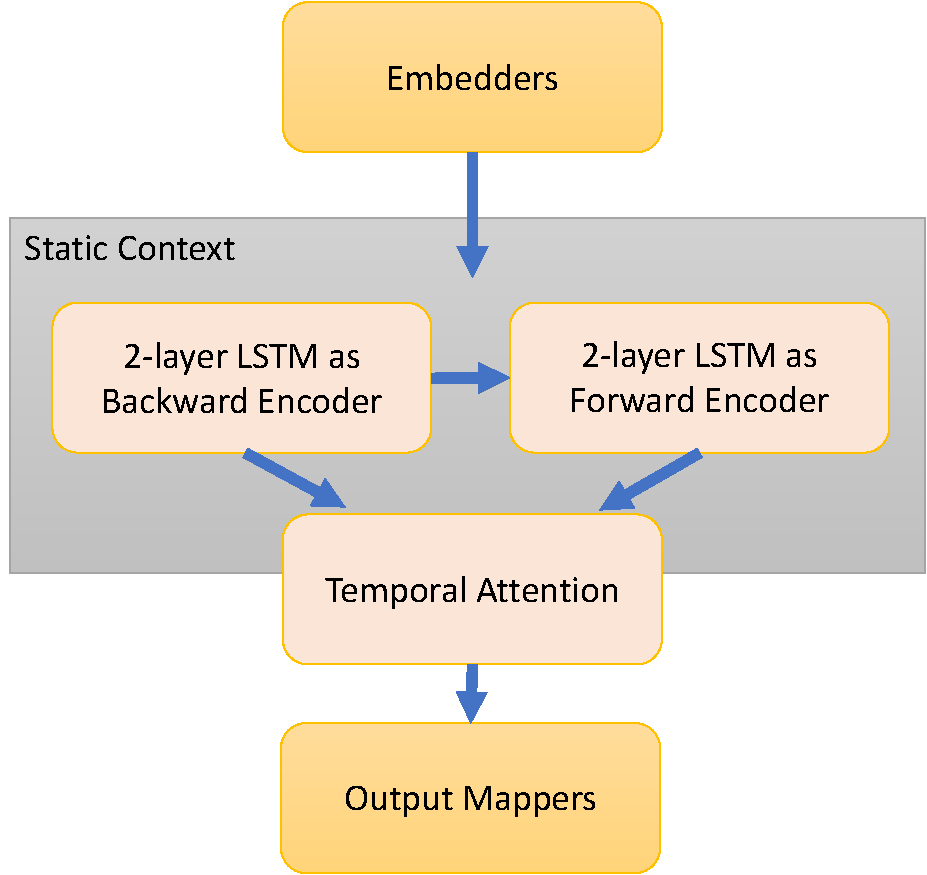
\includegraphics[width=0.5\columnwidth]{images/tft}
    \caption{TFT Model Architecture \citep{fox2022-jm}.}
    \label{fig:TFT_Model_Arch}
\end{figure}


For this paper we adopted the same calculations as defined in \cite{fox2022-jm}: ``We have chosen various samplings of the dataset to provide both input and predicted values. These include time ranges from a fortnight up to 4 years. Further, we calculate summed (according to Equation (1)) magnitudes and averaged depths (according to Equation (2)) and counts of significant earthquakes (magnitude > 3.29, Equation (3)).  We use the concept of {\em energy averaging} when there are multiple events in a single space–time bin. Therefore, the magnitude assigned to each bin is defined in Equation (1) as “log(Energy)” where we sum over events of individual magnitudes $m_{event}$ We also use energy averaging defined in Equation (2) for quantities $Q_{bin}$ such as the depth of an earthquake that needs to be weighted by their importance when averaging over a bin.''

\begin{equation}
m_{bin} = \log(Energy) = \frac{1}{1.5}\log_{10}\sum_{in~bin}^{Events}10^{1.5m_{event}}
\end{equation}

\begin{equation}
Energy~weighted~Quantity~Q_{bin} = \frac{\displaystyle
   \sum^{Events}_{in~bin} 10^{1.5m_{event}} Q_{event}}{\displaystyle \sum^{Events}_{in~bin}1.5m_{event}}
\end{equation}

\begin{equation}
Multiplicity_{bin} = \sum^{Events}_{in~bin}Multiplicity_{event} ~ subject~to~a~constraint
\end{equation}


In this paper, we only focus on the TFT implementation. The TFT Inputs and Outputs are described next \cite{fox2022-jm}.

\begin{itemize}
\item {\bf Static Known Inputs (5 Inputs):} 4 space-filling curve
  labels of fault grouping, linear label of pixel
  \item {\bf Targets (4 Targets):} $m_{bin} (F:\Delta t,t)$ for $\Delta t = 2, 14, 26, 52$ weeks. Calculated for $t-52$ to $t$ for encoder and $t$ to $t+52$ weeks for decoder in $2$ week intervals. 104 predictions per sequence.
  \item {\bf Dynamic Known Inputs (13 Inputs):} $P_l(\cos_{Full})$ for $l=0$ to $4$ $\cos_{period}(t), \sin_{period}(t)$  for $period = 8, 16, 32, 64$
  \item {\bf Dynamic Unknown Inputs (9 Inputs):} Energy-averaged Depth, Multiplicity, Multiplicity  $m>3.29$ events $m_{bin}$ $(B:\Delta t,t)$ for $\Delta$ $t = 2, 4, 8, 14, 26, 52$ weeks
\end{itemize}


This data can be input based on the time series. Backward data can be taken up to 1 year before the current date and forward data can be taken up to 4 years into the future. The data is then enriched with the LSTM models on time and other factors like spacial location, fault grouping and energy produced at location. Feature selection is done. The data is then fed into an attention learning module which learns trends and more complex relationships based on the data across all time steps and can apply this knowledge to any number of time steps. More feature selection is done. Then finally the data is run through quantile regression. The loss is calculated by Mean Absolute Error (MAE). This repeats until all Epoch runs are done and the iteration that had the lowest loss is used to create predictions. Normalized Nash–Sutcliffe Efficiency (NNSE) and Mean Squared Error (MSE) are used as a goodness of fit metric.

More details of the TFT model applied to the earthquake application are presented in ~\citep{fox2022-jm}. More general details about TFT models can be found in~\citep{TFT-21}.


\subsubsection{Insights into Development of the Code}

The original code was developed with the goal to create a DL method called {\em TEvolOp} to apply special time-series evolution for multiple applications including earthquake, hydrology, and COVID prediction. The code was presented in a large Python Jupyter Notebook on Google Colab.  Due to the integration of multiple applications (hydrology and COVID), the code was difficult to understand and maintain. For this reason, the total number of lines of 13500 was reduced by more than 2400 lines when the hydrology and the COVID code were removed. However, at the same time, we restructured the code and reached a final length of about 11100 lines of code. The original code contained all hyperparameters and needed to be changed every time a hyperparameter was modified.  The code included all definitions of variables and hyperparameters in the code itself. The code could be further made shorter by separating the model code into a library.

This code has some issues that future versions ought to address. First, the code includes every aspect that is not covered by TensorFlow and also contains a customized version of TFT. Second, due to this the code is very large, and manipulating and editing the code is time-consuming and error-prone. Third, as many code-related parameters are managed still in the code running the same code with various parameters becomes cumbersome. In fact, multiple copies of the code need to be maintained when new parameters are chosen, instead of making such parameters part of a configuration file. Hence we started moving towards the simplification of the code by introducing the concept of libraries that can be pip installed, as well as adding gradually more parameters to configuration files that are used by the program.

The advantage of using a notebook is that it can be augmented with lots of graphs that give updates on the progress and its measurement accuracy. It is infeasible for students to use and replicate the run of this notebook on their own computers as the runtime can be up to two days. Students use their computers for other purposes and need to be able to use them on the go. Often HPC centers provide interactive jobs in the batch queues, but this is also insufficient. Instead, we opted to use Jupyter notebooks with a special batch script that internally uses Papermill \citep{www-papermill} and leverage an HPC queueing system to execute the notebook in the background. Papermill will also include all cells that have to be updated during runtime, including graphics. The script we developed needed to be run multiple times and with different hyperparameters such as the number of epochs.  As the HPC system is a heterogeneous GPU system having access to A100, V100, P100, and RTX2080 graphics cards, the choice of the GPU system must be able to be configurable. Hence, the batch script includes the ability to also read in the configuration file and adapt itself to the needed parameters. This is controlled by a sophisticated but simple batch job generator which we discuss in Section~\ref{sec:workflow-sbatch}.

%libraries for mlcommons benchmarking, cloudmesh
%portable way to define data locations via config
%experiment permutation over hyperparameters.
%* repeated experiments
%* separate evaluation and comparison of accuracy which was not in the original code.
%* comparison of accuracy across different hyperparameter searches.


\subsection{Insights into Data Management from the Earthquake Forecasting Application}
\label{sec:eq-data}

In data management, we are concerned with various aspects of the data set, the data compression and storage, as well as the data access speed. We discuss insights into each of them next.

\subsubsection{Data Sets}


When dealing with datasets we typically encounter several issues.  These issues are addressed by the MLCommons benchmarks and data management activities so that they provide ideal candidates for education without spending an exorbitant amount of time on data. Such issues typically include access to data without privacy restrictions, data preprocessing that makes the data suitable for deep learning, data labeling in case they are part of a well-defined MLCommons benchmark. Other issues include data bias, noisy or missing data, as well as overfitting while using training data. Typically the MLCommons benchmarks will be designed to limit such issues. However, some benchmarks such as the science group benchmarks which are concerned with improving the science have the option to potentially address these issues in order to improve the accuracy. This could include even injecting new data and different preprocessing methods.


\subsubsection{Data Compression}

An issue of utmost importance, especially for large data sets, is how the data is represented. For example, we found that the original dataset was 11GB big for the earthquake benchmark. However, we found the underlying data was a sparse matrix, and was easily compressed by a factor of 100 with lossless compression. This is significant, as in this case the entire dataset can be stored in GitHub or moved quickly into memory. The compressed xz archive file is only 21 MB and downloading only the archive file using wget takes 0.253s on the HPC. In case the dataset and its repository are downloaded with Git, we note that the entire Git repository is 108MB~\citep{eq-data}. On the RIvanna Supercomputer, downloading this compressed dataset only takes 7.723s. Thus, it is preferred to just download the data using wget. In both cases, the data is compressed. To uncompress, the data it will take an additional 1 minute and 2.522 seconds. However, if we were to download the data in uncompressed form it would take approximately 3 hours and 51 seconds. This is due to the fact that the data is sparse and the compression allows a significant reduction needed to store this data.

From this simple example, it is clear that MLCommons benchmarks can provide students insights into how data is managed and delivered to for example large-scale computing clusters with many nodes while utilizing compression algorithms. We will next discuss insights into infrastructure management while using filesystems in HPC resources.  While often object stores are discussed to host such large datasets it is imperative to identify the units of storage in such object stores.  In our case, an object store that would host individual data records is not useful due to the vast number of data points. Therefore the best way to store this data even in an object store is as a single entry of compressed overall data.  Other MLCommons Science working group benchmarks have datasets in the order of 500GB to 12TB. Other tools, such as Globus transfer, can be used to download larger datasets.  Obviously, these sets need special considerations when placed on a computing system where the students' storage capacities may be limited by policy.


\subsubsection{Data Access}

Besides having proper data and being able to download it efficiently from the location of storage, it is imperative to be able to access it in such a way that the GPUs used for deep learning are being fed with enough data without being idle. Our performance results were somewhat surprising and had a devastating effect on the overall execution time. We found that the performance was more than twice as fast on the personal computer while using an RTX3090 in contrast to using the HPC center recommended filesystems when using an A100. For this reason, we have made a simple test and measured the performance to read access the various file systems. The results are shown in Table~\ref{tab:file-performance} which include various file systems at the University of Virginia's Rivanna HPC but also a comparison with a personal computer.

\begin{comment}
\begin{table}[htb]
  \caption{File transfer performance of various file systems on Rivanna and personal computers.}
  \label{tab:file-performance}
  \begin{center}
  {\footnotesize 
  \begin{tabular}{|llrrrp{4.5cm}|}
    \hline
    Machine & File systems & \multicolumn{2}{l}{Bandwidth Performance} & Speedup & Description \\
    \hline
    \hline
    Rivanna & \verb|/scratch/$USER  (sbatch)|     & 30.6 MiB/s & 32.1 MB/s  & 1.0 & shared scratch space, batch mode \\
    Rivanna & \verb|/scratch/$USER (interactive)| & 33.2 MiB/s &  34.8 MB/s  & 1.1 & shared scratch space, interactive \\
    Rivanna & \verb|/home/$USER|                    & 40.9 MiB/s & 42.9 MB/s  & 1.3 & users home directory \\
    MacM1   & \verb|/| & 93.2MiB/s & 97.7MB/s & 3.0 & users homedir \\
    Rivanna & \verb|/project/$PROJECTID |     & 100 MiB/s  & 105 MB/s  & 3.3 & project specific filesystem \\
    Personal Computer  & \verb|c:| & 187 MiB/s  & 196 MB/s  & 6.1 &  file system on a personal computer \\
    Rivanna & \verb|/tmp|                         & 271 MiB/s  & 285 MB/s  & 8.9 & temporary file system on a node \\
    \hline
    Special Node Rivanna & \verb|/localscratch|  &  384 MiB/s & 403 MB/s  & 12.6 & NVMe storage of the node\\
    RAM disk Rivanna  & \verb|/dev/shm/*|      &             461 MiB/s & 483 MB/s  & 15.1 & simulated filesystem in a RAM disk\\
    Personal Computer & \verb|/home/$USER| & 579 MiB/s & 607 MB/s &  18.9 & Sabrent 2TB NVMe\\
    \hline                                             
    \end{tabular}
  }
    \end{center}
\end{table}
\end{comment}

\begin{table}[htb]
  \caption{File transfer performance of various file systems on Rivanna and personal computers.}
  \label{tab:file-performance}
  \begin{center}
  {\footnotesize 
  \begin{tabular}{|llrrrp{4.5cm}|}
    \hline
    Machine & File systems & Bandwidth & Speedup & Description \\
    \hline
    \hline
    Rivanna & \verb|/scratch/$USER  (sbatch)|     &  32.1 MB/s  & 1.0 & shared scratch space, batch mode \\
    Rivanna & \verb|/scratch/$USER (interactive)| &  34.8 MB/s  & 1.1 & shared scratch space, interactive \\
    Rivanna & \verb|/home/$USER|                    & 42.9 MB/s  & 1.3 & users home directory \\
    MacM1   & \verb|/| &  97.7MB/s & 3.0 & users homedir \\
    Rivanna & \verb|/project/$PROJECTID |     &  105 MB/s  & 3.3 & project specific filesystem \\
    % Personal Computer  & \verb|c:| &  196 MB/s  & 6.1 &  file system on a personal computer \\
    Rivanna & \verb|/tmp|                         &  285 MB/s  & 8.9 & temporary file system on a node \\
    \hline
    Special Node Rivanna & \verb|/localscratch|  &  403 MB/s  & 12.6 & NVMe storage of the node\\
    RAM disk Rivanna  & \verb|/dev/shm/*|      &    483 MB/s  & 15.1 & simulated filesystem in a RAM disk\\
    Personal Computer & \verb|/home/$USER| &  607 MB/s &  18.9 & Sabrent 2TB NVMe\\
    \hline                                             
    \end{tabular}
  }
    \end{center}
\end{table}
  


Based on this observation, it was of great disadvantage to consider running the earthquake benchmark on the regularly configured HPC  nodes as they ran on some resources for almost 24 hours due to the policy limit the Rivanna system allows for one job. Hence, we were allowed to use a special compute node that has additional NVMe storage available and accessible to us. On those nodes (in the Table listed as \verb|/localscratch|), we were able to obtain a very suitable performance for this application while having a 10 times fold increase in access in contrast to the scratch file system and almost double the performance given to us on the project file system. The \verb|/tmp| system -- although fast -- was not sufficiently large for our application and also performs slower than the \verb|/localscratch| set up for us. In addition, we also made an experiment using a shared memory-based hosted filesystem in the nodes RAM.

What we learn from this experience is that an HPC system must provide a fast file system locally available on the nodes to serve the GPUs adequately. The computer should be designed from the start to not only have the fastest possible GPUs for large data processing but also have a very fast filesystem that can keep up with the data input requirements presented by the GPU. Furthermore, in case updated GPUs are purchased, it is not sufficient to just take the previous generation motherboard and CPU processor and memory but to update the hardware components and include a state-of-the-art compute node. This often prevents the repurposing of the node while adding just GPUs due to inefficient hardware components that can not keep up with the GPUs capabilities.

  


\subsection{Insights into DL Benchmark Workflows}
\label{sec:workflow-main}

As we are trying to benchmark various aspects of the applications and the systems utilizing Deep Learning, we need to be able to easily formulate runtime variables that take into account different control parameters either of the algorithm or the underlying system and hardware.

Furthermore, it is beneficial to be able to coordinate benchmarks on remote machines either on a single system or while using multiple systems in conjunction with hybrid and heterogeneous multi-HPC systems. These concepts are similar to those found in cloud and Grid computing for job services \citep{las-infogram} and for workflows \citep{las-workflow,las07-workflow}. However, the focus here is that the services provided are controlled by the application user and not necessarily by the cloud or HPC provider. Thus we distinguish the need for a workflow service that can utilize heterogeneous HPC systems while leveraging the same parameter set to conduct a benchmark for comparison. Such a framework was presented by von Laszewski, Fleischer, et al. in \citep{las-22-arxiv-workflow-cc} and is based on our earlier work on workflows in clouds and Grids.

In addition, we need a mechanism to create various runs with different parameters. One of the issues we run into is that often our runtime needs exceed that of a single job submission. Although job arrays and custom configurations exist, they often lead to longer run times that may not be met by default policies used in educational settings. Thus it is often more convenient to create jobs that fall within the limits of the HPC center's policies and split the benchmarking tasks across a number of jobs based on the parameter permutations. This allows also easier parallelization.

For this reason, von Laszewski, Knuuti, et al. have implemented {\it
  cloudmesh-sbatch} that provides a batch job generator, creating parallel jobs based on a permutation of experiment parameters that are defined in a configuration file. The tool will create for each job its own subdirectory, copies the code and configuration files into it, and creates a shell script that lists all jobs to be submitted to the queuing system.

Furthermore, we need a simple system to measure the performance and energy, while communicating the data in an easy fashion to the users. This system was developed by von Laszewski and contains two components (a) a general stopwatch (b) a mechanism to monitor the GPU as discussed in \ref{sec:monitoring}.

We describe these systems briefly while focusing on their applicability for benchmarks.

\subsubsection{Cloudmesh Monitoring}
\label{sec:monitoring}

To conduct monitoring of time we have provided for years a convenient StopWatch package in Python \citep{cloudmesh-stopwatch}.  It is very easy to use and is focused on runtime execution monitoring of time-consuming portions in a single-threaded Python application. Although MLCommons provides their own time measuring component, called mllog, it is clear from the name that the focus is to create entries in a log file that is not easily readable by a human and may require post-processing to make it usable. In contrast, our library contains not only simple labeled \verb|start| and \verb|stop| methods, it also provides a convenient mechanism to print human-readable customizable performance tables. However, it is possible to also generate a result table in other formats such as CSV, JSON, YAML, TXT, and others).  Human readability is especially important during a debugging phase when benchmarks are developed. Moreover, we also have developed a plugin interface to mllog, that allows us to automatically create mllog entries into an additional log file, so the data may be used within MLCommons through specialized analytics programs. A use case is depicted next (we have omitted other advanced features such as function decorators for the StopWatch to keep the example simple).

{\fontsize{6pt}{6pt}\selectfont
\begin{lstlisting}[style=python]
    from cloudmesh.common.StopWatch import StopWatch 
    # ...
    StopWatch.event("start")       # this where the timer starts
    StopWatch.start("earthquake")  # this is when the main benchmark starts
    # ... run the earthquake code
    # ... additional timers could be used here
    with StopWatchBlock("calc"):   # this is how to use a block timer
       run_long_calculation()
    StopWatch.stop("earthquake")   # this is where the main benchmark ends
    StopWatch.benchmark()          # prints the current results
\end{lstlisting}
}

To have also direct access to MLCommons events, we have recently added the ability to call a StopWatch.event.


In addition to the StopWatch, we have developed a simple command line tool that can be used for example in batch scripts to monitor the GPU performance characteristics such as energy, temperature, and other parameters \citep{cloudmesh-gpu}. The tool can be started in a batch script as follows and is currently supporting NVIDIA GPUs:

{\fontsize{6pt}{6pt}\selectfont
\begin{lstlisting}[style=sh]
    cms gpu watch --gpu=0 --delay=0.5 --dense > gpu0.log &
\end{lstlisting}
}


Monitoring time and system GPU information can provide significant insights into the application's performance characteristics. It is significant for planning a time-effective schedule for parameters while running a subset of planned experiments.


\subsubsection{Analytics Service Pipelines}

In many cases, a big data analysis is split up into multiple subtasks. These subtasks may be reusable in other analytics pipelines. Hence it is desirable to be able to specify and use them in a coordinated fashion allowing the reuse of the logic represented by the analysis. Users must have a clear understanding of what the analysis is doing and how it can be invoked and integrated.

The analysis must include an easy-to-understand specification that encourages reuse and provides sufficient details about its functionality, data dependency, and performance. Analytics services may have authentication, authorization, and access controls built-in that enable access by users controlled by the service providers.

The overall architecture is depicted in Figure \ref{fig:cc-2}A. It showcases a layered architecture with components dealing with batch job generation, storage management, compute coordination, and monitoring. These components sit on top of other specialized systems that can easily be ported to other systems while using common system abstractions.

\begin{figure}[htb]
    \centering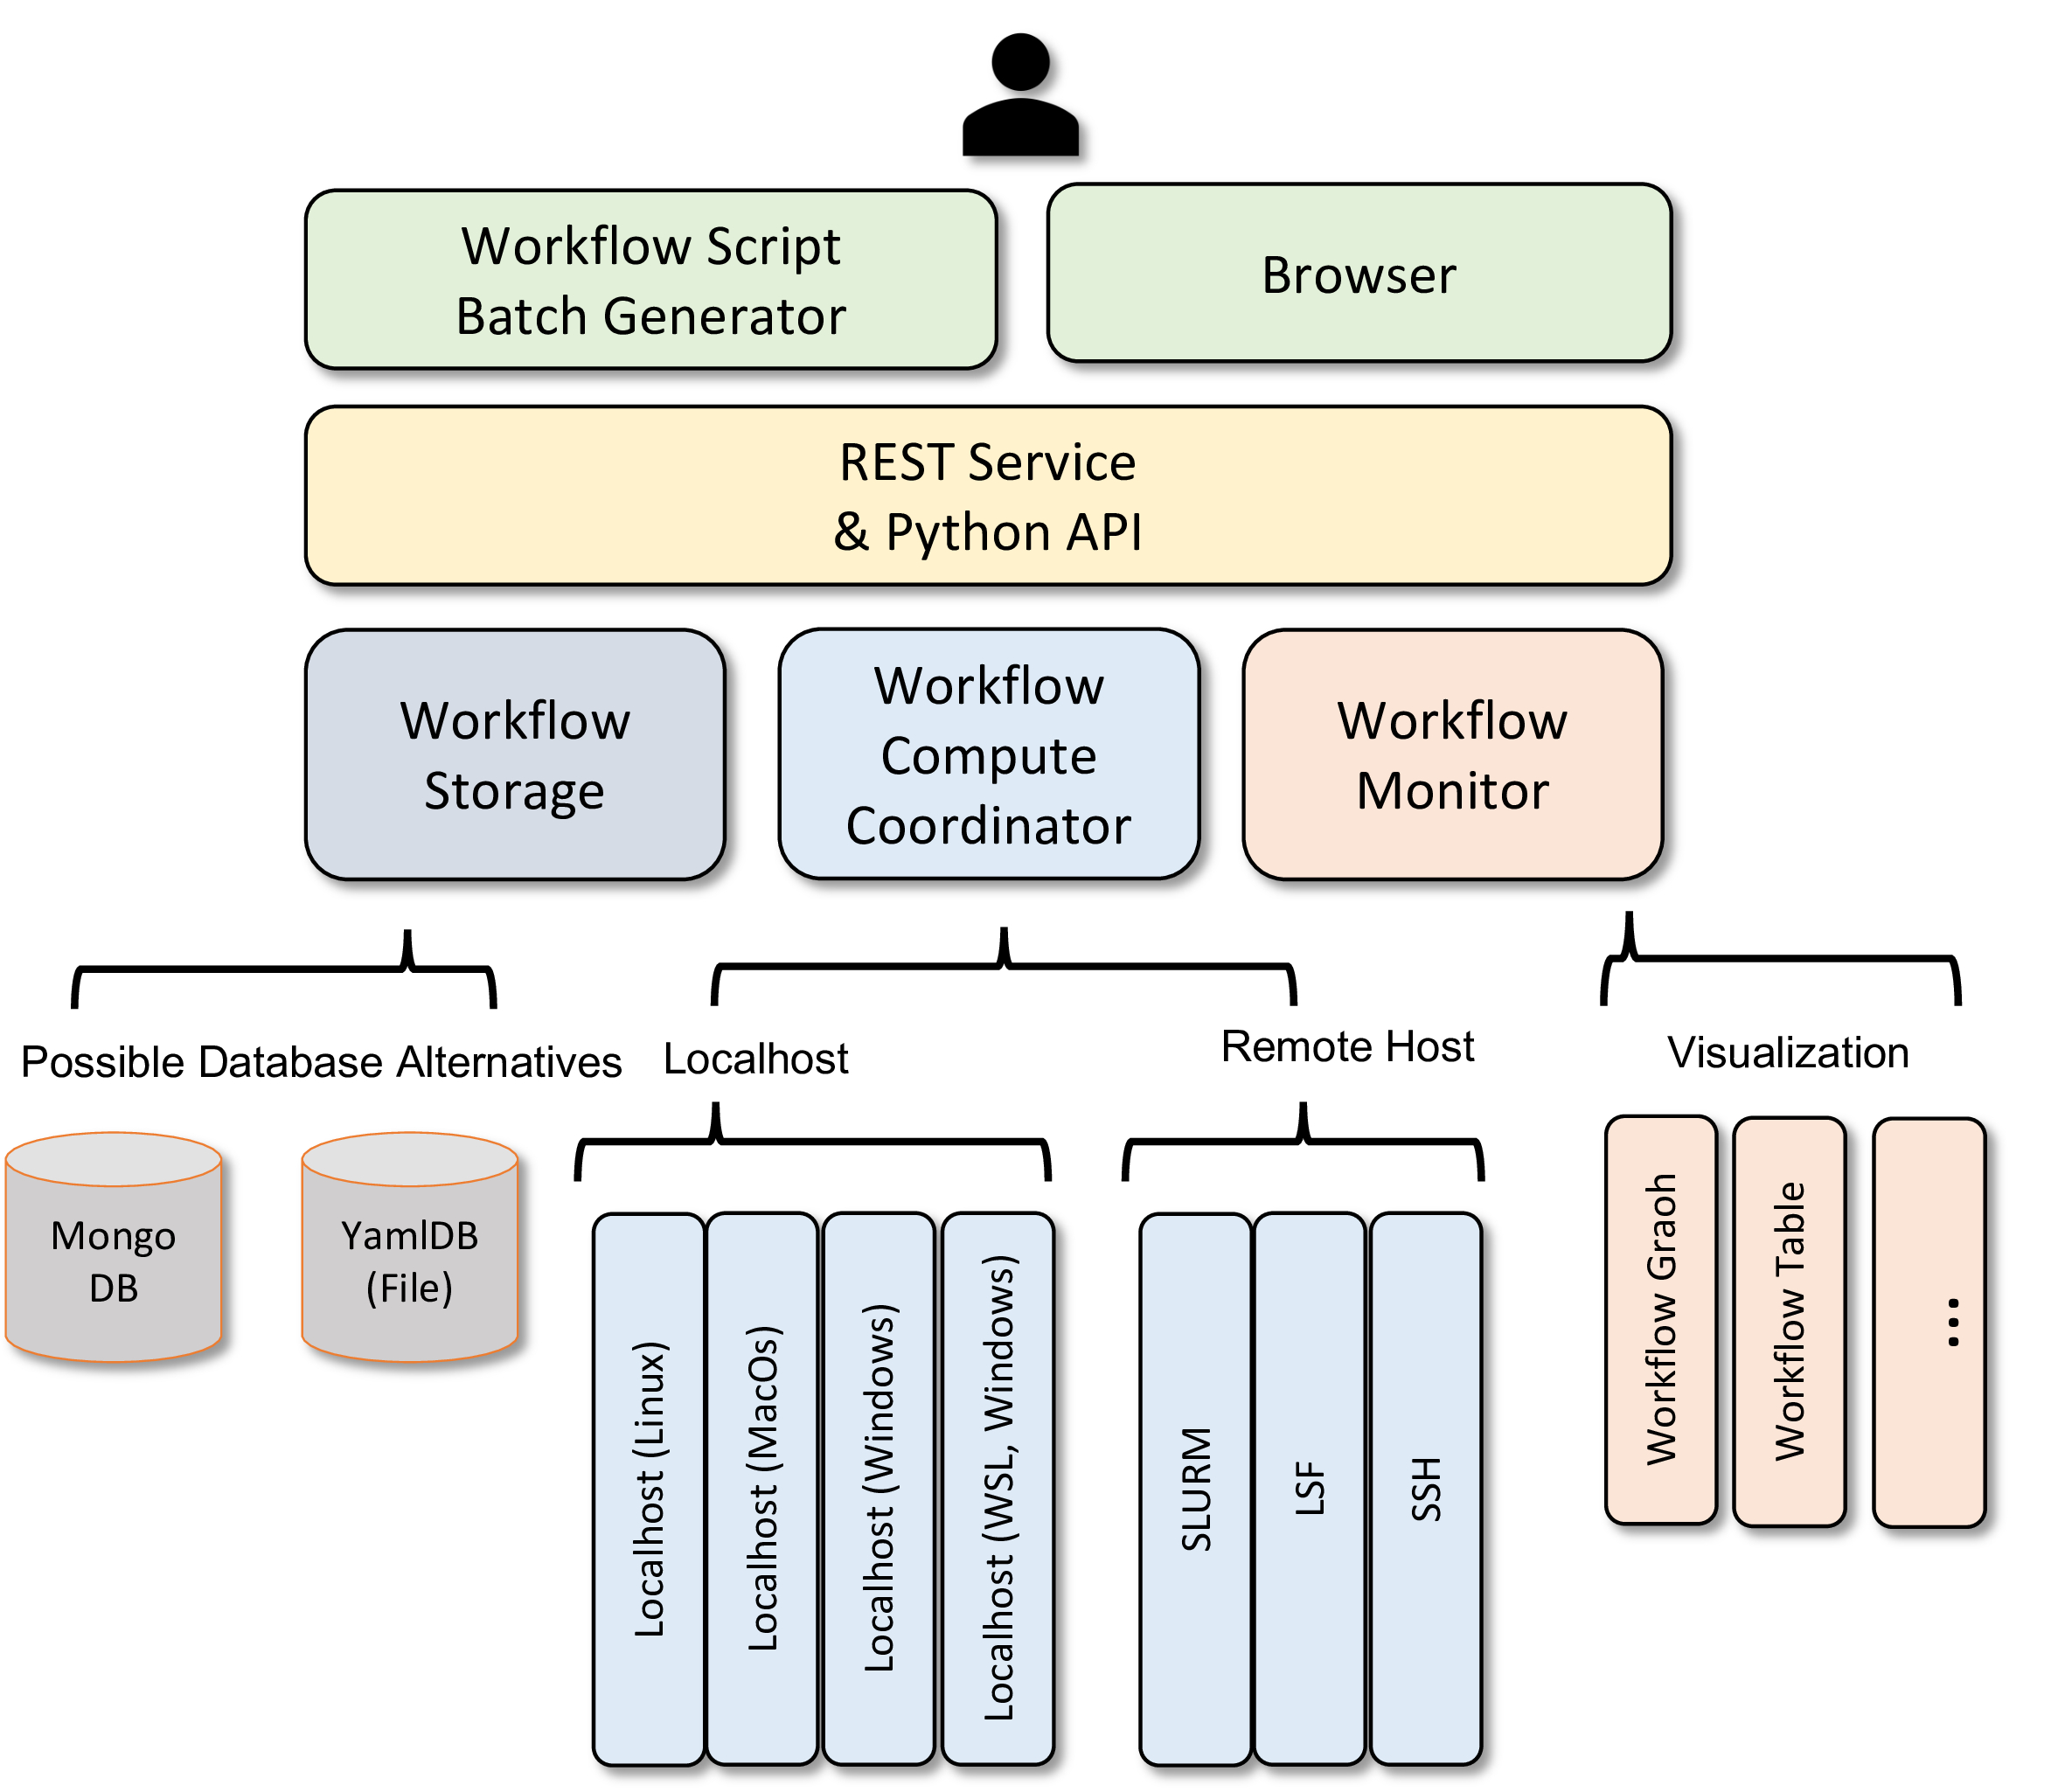
\includegraphics[width=0.70\columnwidth]{images/cloudmesh-cc-new}
    
    {\bf (A)} Architecture of the overall workflow framework.

\bigskip\bigskip
    
    \centering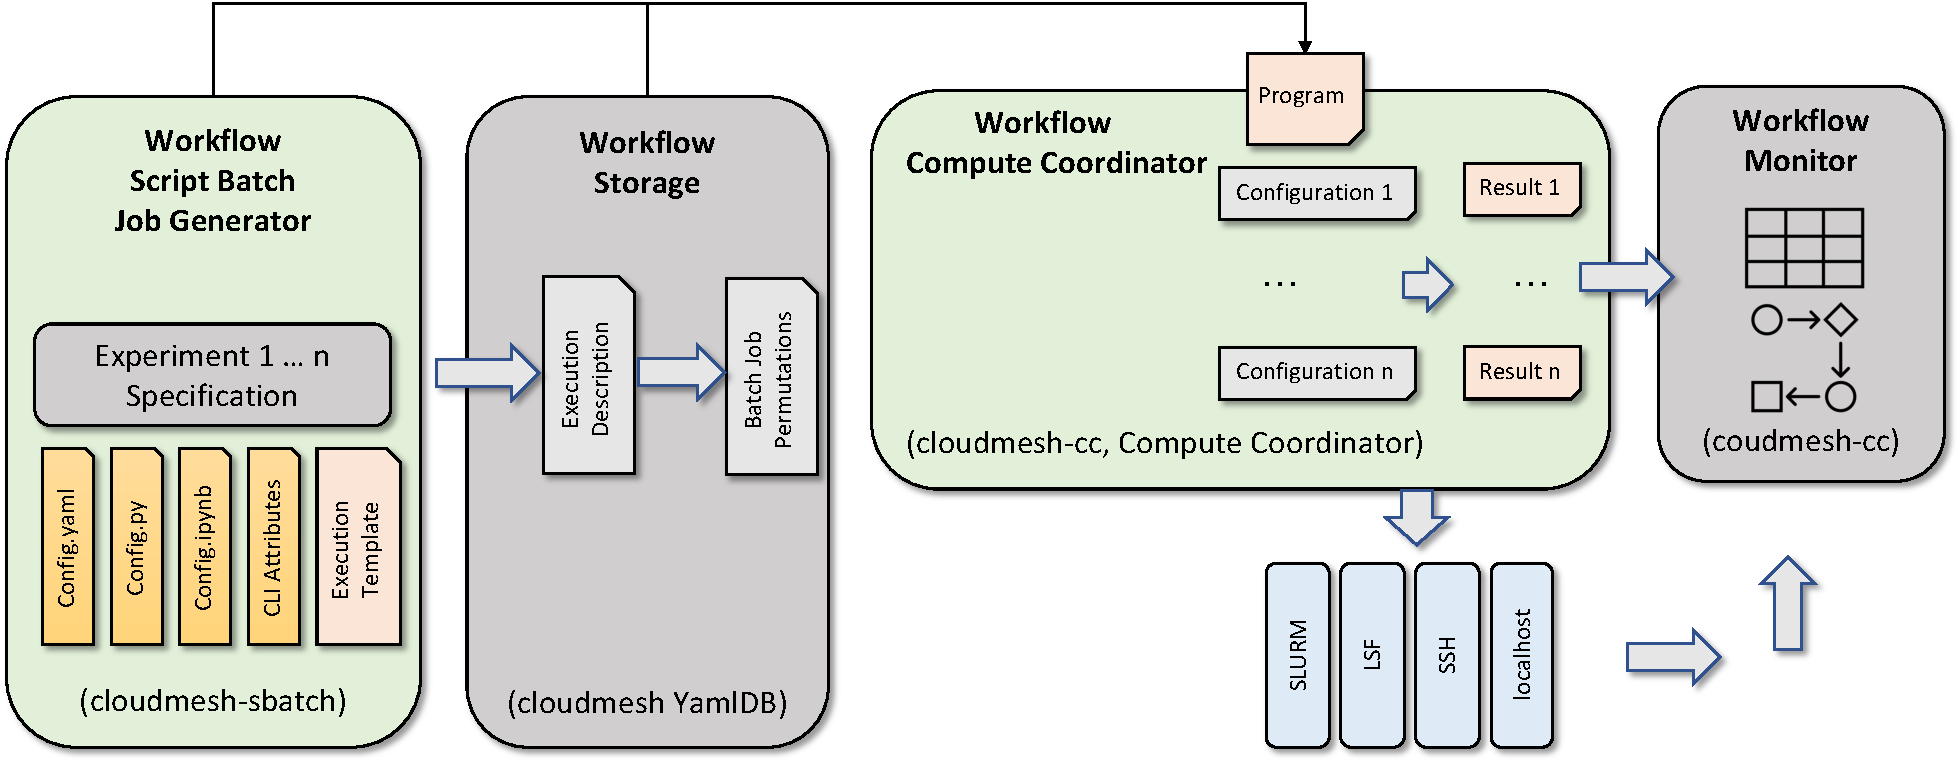
\includegraphics[width=1.0\columnwidth]{images/cloudmesh-sbatch-new}
    
    
    {\bf (B)} Architecture of Workflow Script Batch Generator cloudmesh-sbatch.

    \caption{Architecture of the Cloudmesh Workflow Service Framework.}
    \label{fig:cc-2}

\end{figure}

Instead of focusing on the details of this architecture, we found that the high-level use of it is very important as part of the educational activities which also have an implication in general on the use within any research activity.

We identified three beneficial concepts as part of the analytics service pipelines (see Figure \ref{fig:service-interaction}).

\begin{itemize}
\item {\bf Selection} -- Instead of performing all possible benchmarks,  a specific parameter set is selected and only that is run.  \item {\bf Competition} -- From a number of runs, a result is identified that is better than others. This may be, for example, the best of {\em n} benchmark runs.
\item {\bf Cooperation} -- A number of analytics components are run  (possibly in parallel) and the final result is a combination of the benchmark experiments run in cooperation. This for example could be that the job is split across multiple jobs due to resource limitations.
\end{itemize}

In the earthquake code, we have observed all three patterns are used in the benchmark process.

\begin{figure}[htb]
\centering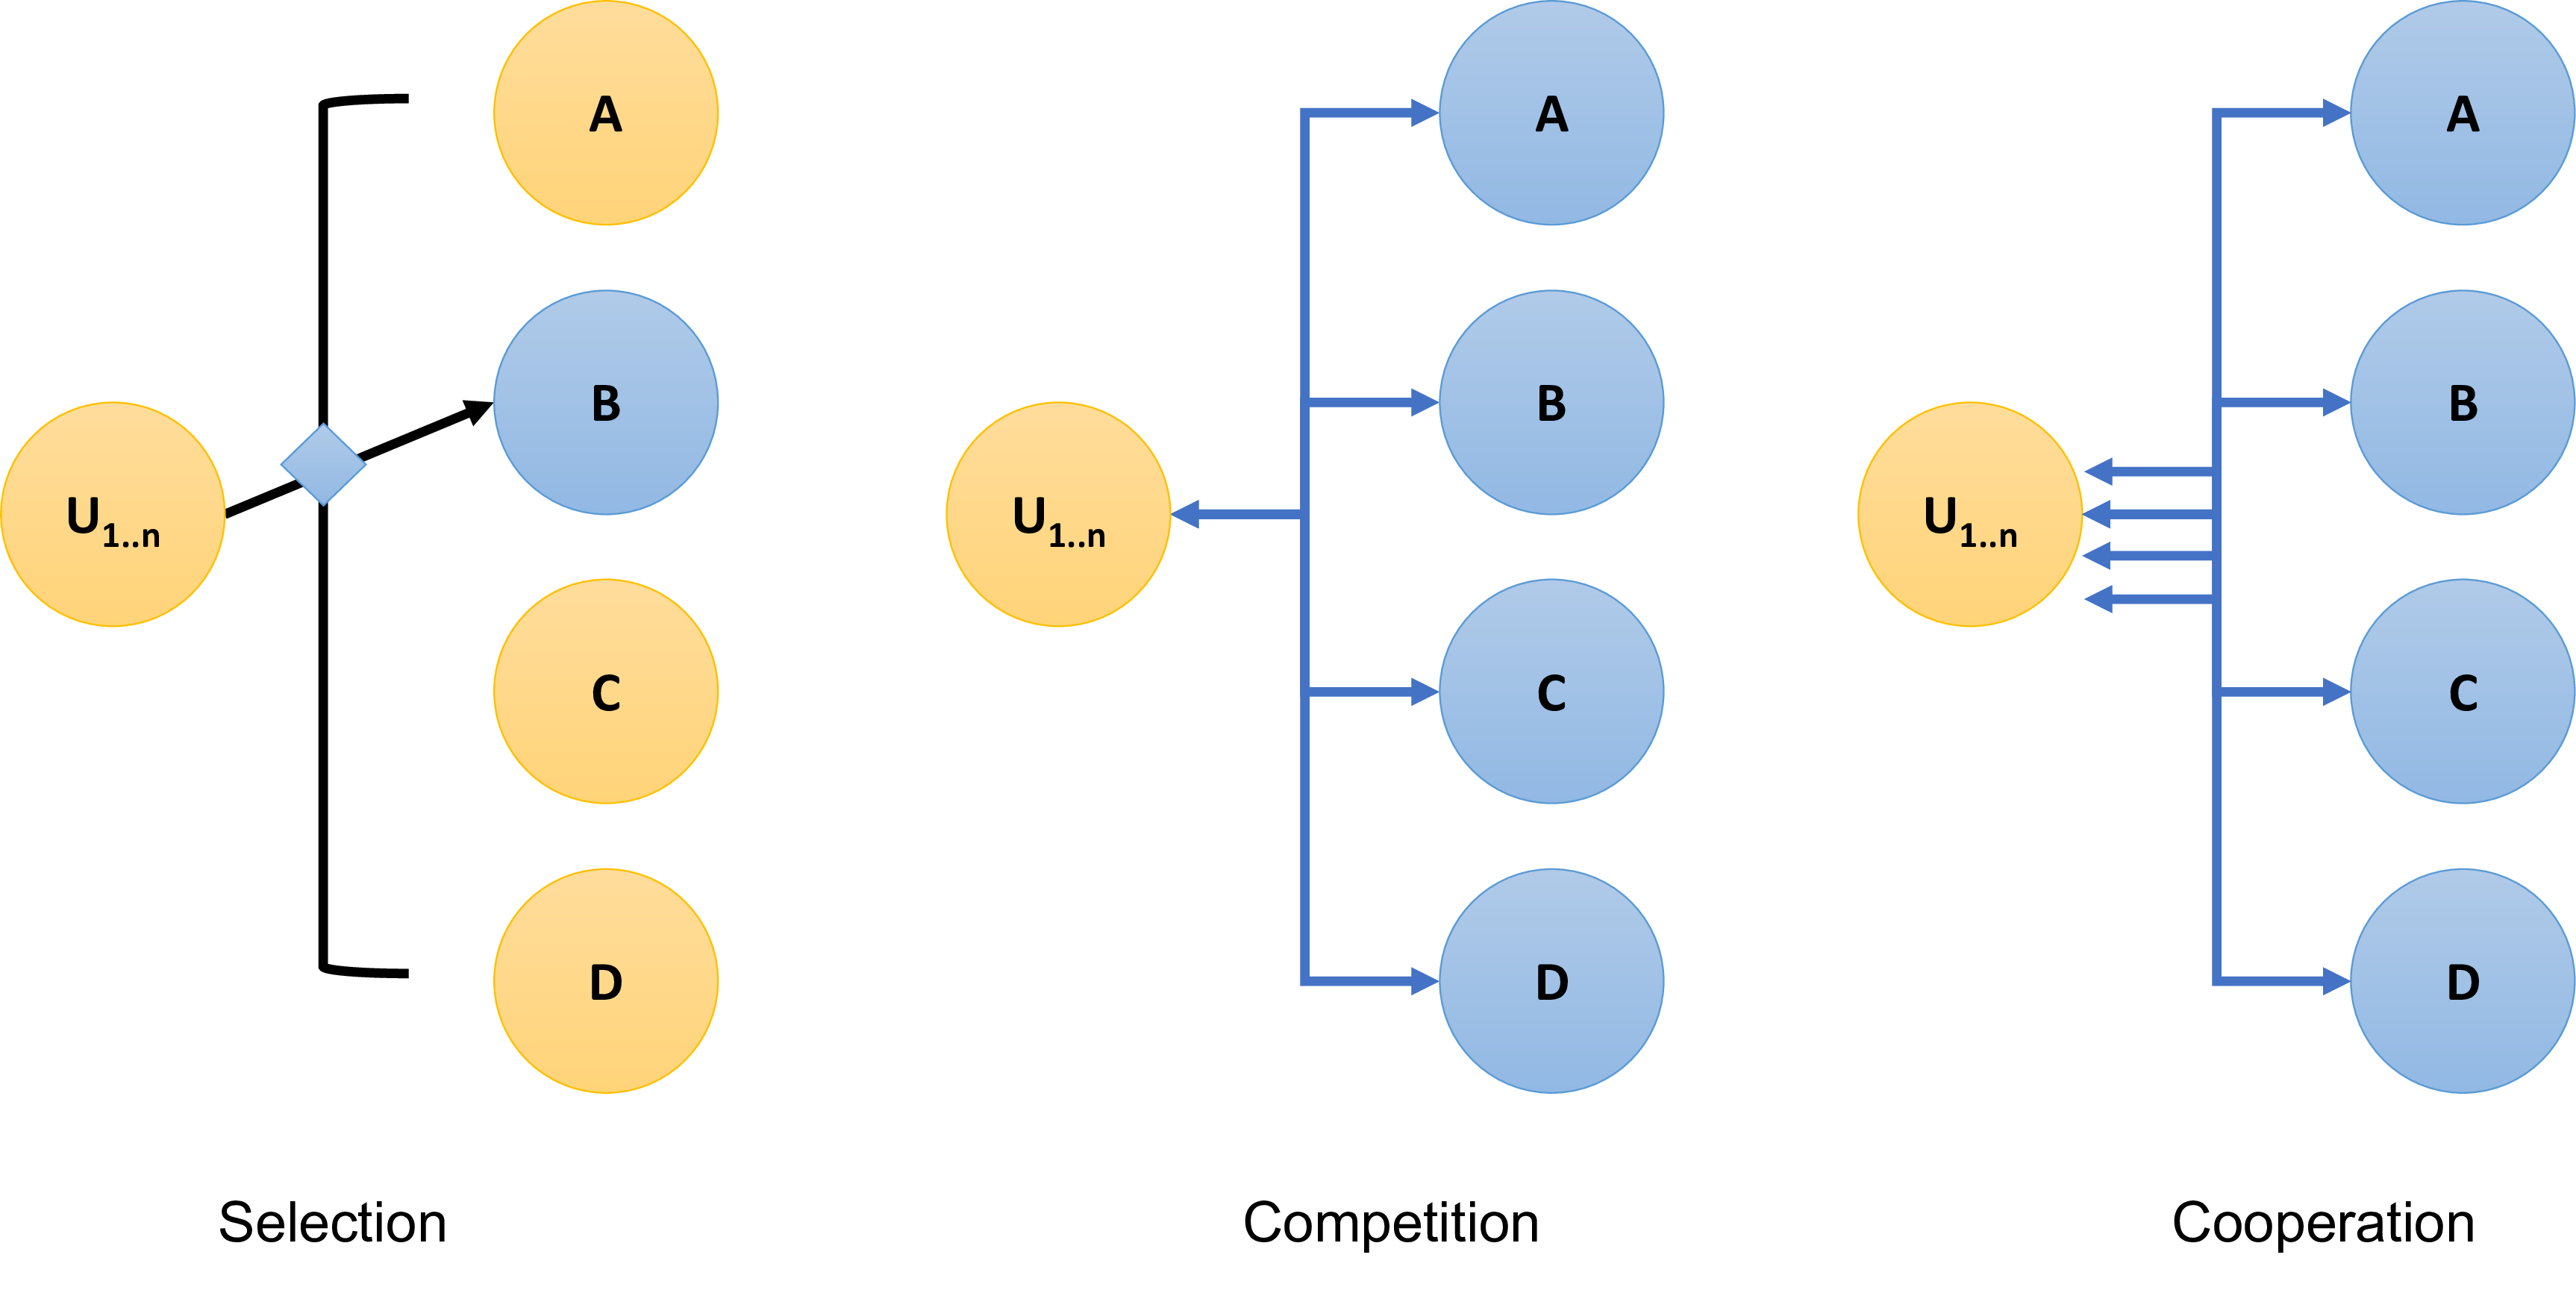
\includegraphics[width=0.75\columnwidth]{images/processes-nist}
\caption{Service Interaction.}
\label{fig:service-interaction}
\end{figure}




\subsubsection{Workflow Compute Coordinator}
\label{sec:workflow-cc}

% possibly some repetition here

High-performance computing (HPC) is for decades a very important tool for science. Scientific tasks can be leveraging the processing power of a supercomputer so they can run at previously unobtainable high speeds or utilize specialized hardware for acceleration that otherwise are not available to the user. HPC can be used for analytic programs that leverage machine learning applied to large data sets to, for example, predict future values or to model current states. For such high-complexity projects, there are often multiple complex programs that may be running repeatedly in either competition or cooperation.  This may include resources in the same or different data centers. We developed a hybrid multi-cloud analytics service framework that was created to manage heterogeneous and remote workflows, queues, and jobs.  It can be used through a Python API, the command line, and a REST service. It is supported on multiple operating systems like macOS, Linux, and Windows 10 and 11.  The workflow is specified via an easy-to-define YAML file.  Specifically, we have developed a library called Cloudmesh Compute Coordinator (cloudmesh-cc) \citep{las-22-arxiv-workflow-cc} that adds workflow features to control the execution of jobs on remote compute resources, while at the same time leveraging capabilities provided by the local compute environments to directly interface with graphical visualizations better suited for the desktop. The goal is to provide numerous workflows that in cooperation enhance the experience of the analytics tasks. This includes a REST service (see Figure \ref{fig:cc-3}A) and command line tools to interact with it.


\begin{figure}[htb]
  \centering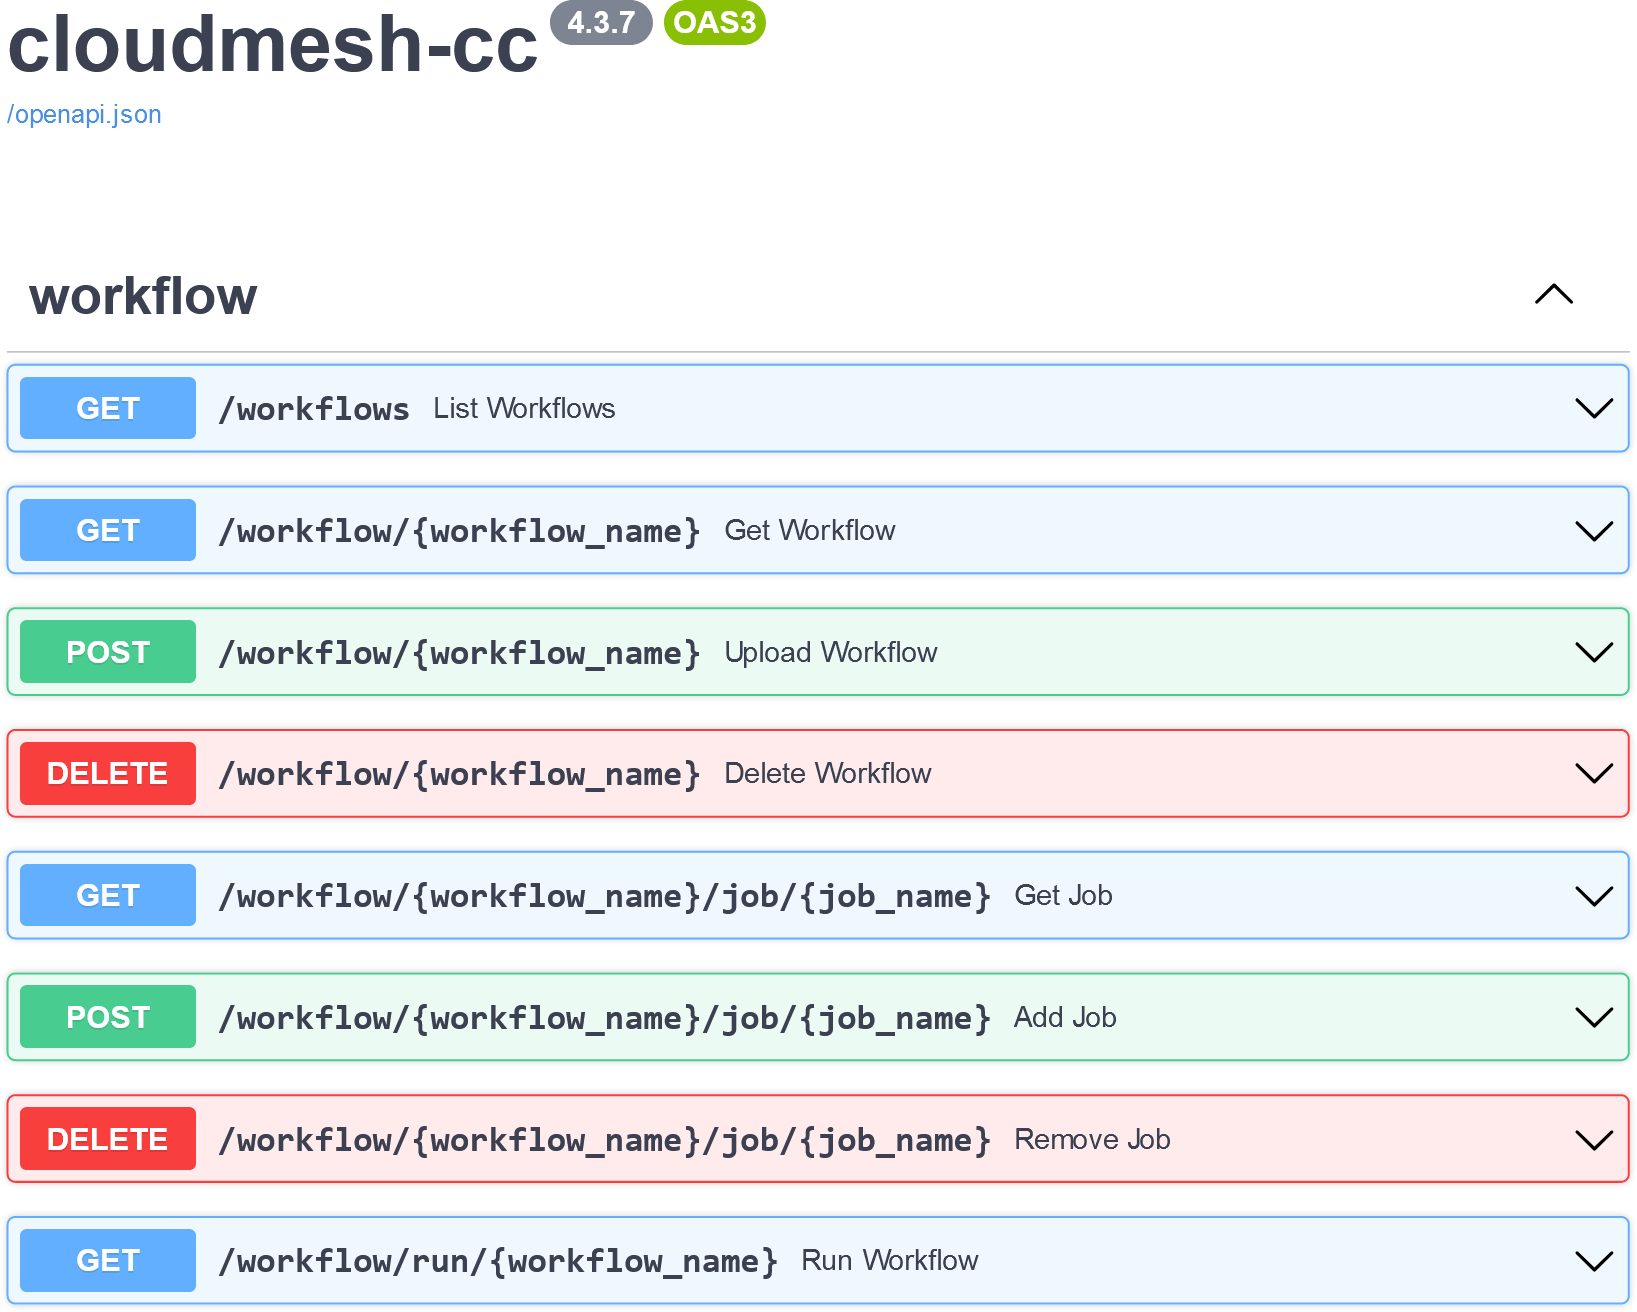
\includegraphics[width=0.8\columnwidth]{images/fastapi-service-highres.jpg}
  
  {\bf (A) Fast API workflow service.}

  \bigskip


    \centering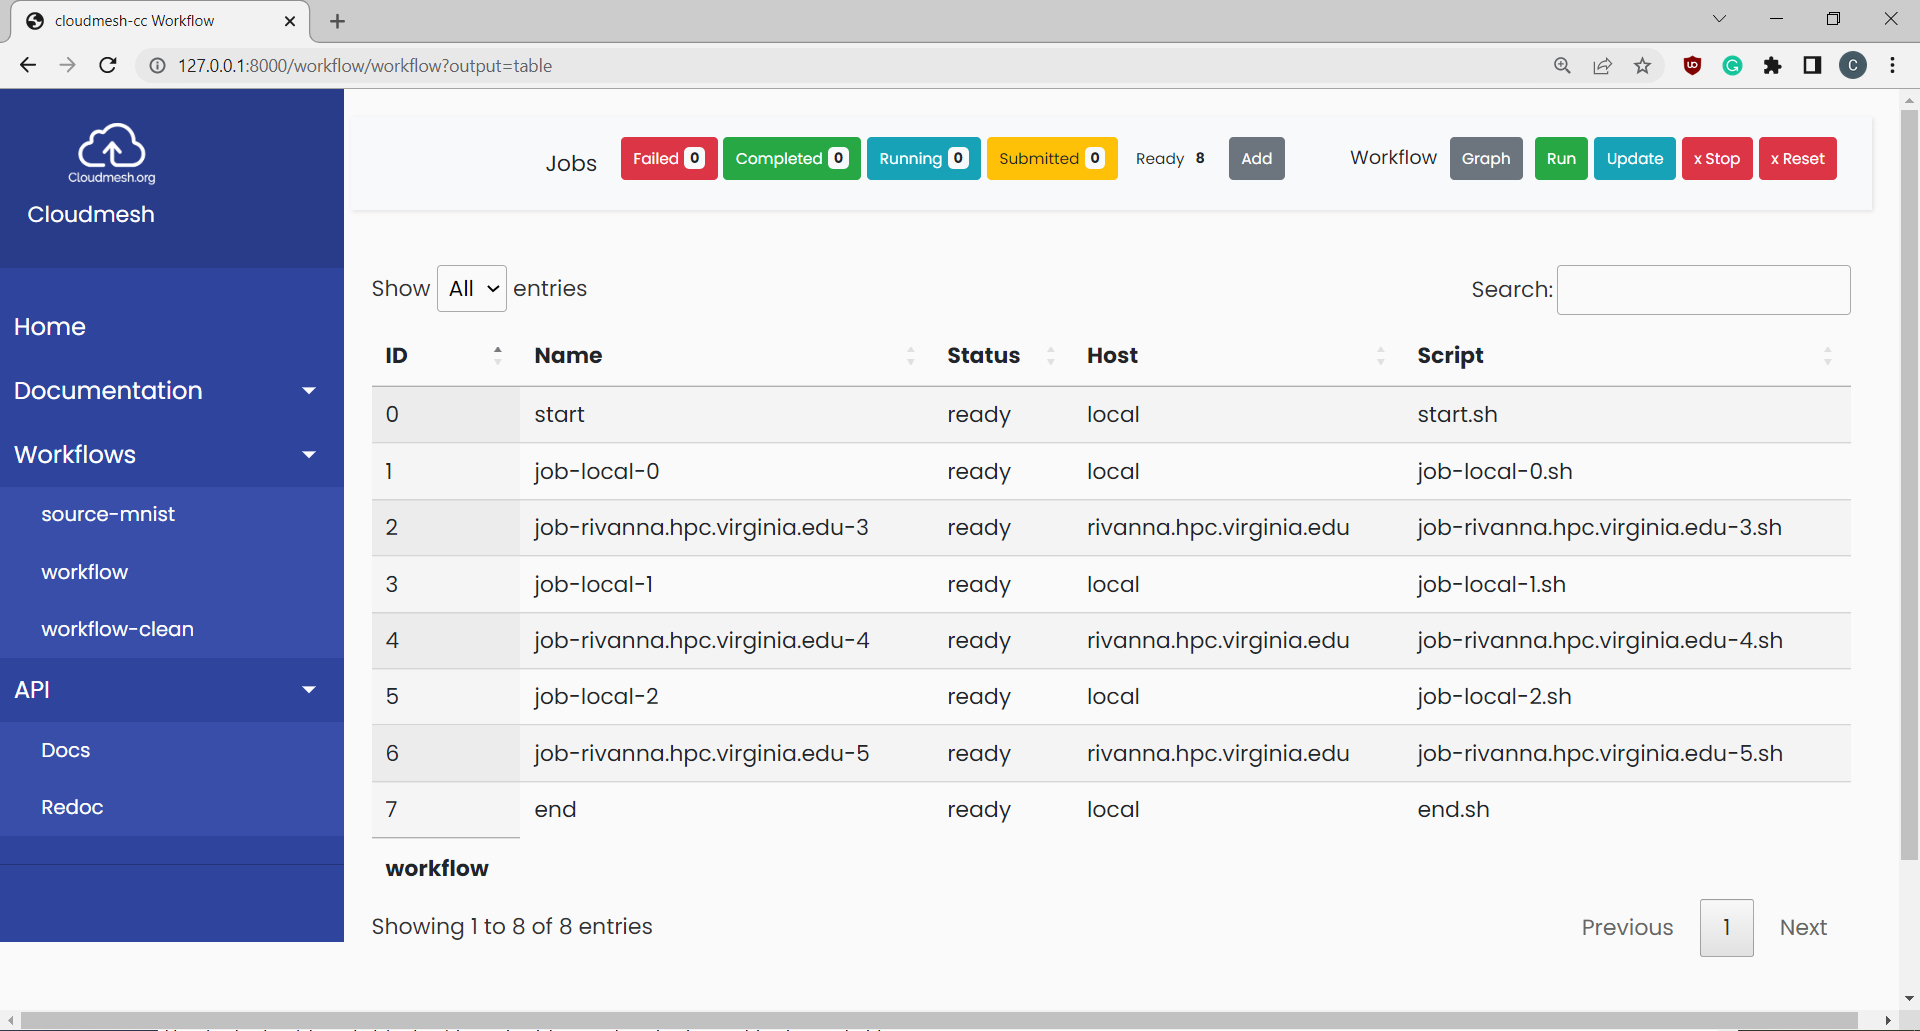
\includegraphics[width=0.8\columnwidth]{images/cc-1.jpg}

    {\bf (B) Workflow user interface.}

    \caption{Workflow interfaces.}
    \label{fig:cc-3}
\end{figure}


We have tested the framework while running various MNIST application examples, including Multilayer Perceptron, LSTM (Long short-term memory), Auto-Encoder, Convolutional, and Recurrent Neural Networks, Distributed Training, and PyTorch training.  A much larger application using earthquake prediction has also been used.

Figure \ref{fig:cc-3}A shows the REST specification and \ref{fig:cc-3}B shows the graphical user interface.

\subsubsection{Parameterized Experiment Workflow Job Generator}
\label{sec:workflow-sbatch}

In traditional machine learning workflows, hyperparameter tuning and configuration are key elements in assessing and optimizing the performance of models. However, scaling hyperparameters for highly parallel execution with heterogeneous hardware is complex.

Cloudmesh-sbatch is a hyperparameter and configuration management toolkit designed to address the generation of batch jobs with a consistent and configurable interface based on hyperparameter values across multiple development toolchains. One of its functions is to create batch jobs based on parameterized job specifications and configuration files.  Cloudmesh-sbatch is part of the Cloudmesh toolkit, a set of tools and libraries for managing cloud and HPC resources from the command line, REST interfaces, or GUI's.  Cloudmesh-sbatch can use a variety of queuing systems and submission commands. Currently, we provide interfaces to Slurm, LSF, and ssh. As the original system was developed first for Slurm sbatch submissions we used the name cloudmesh-sbatch. In the future, we may find a better name showcasing the generality of the system while using arbitrary queuing systems and submission commands.

The architecture of the cloudmesh-sbatch framework is depicted in Figure \ref{fig:cc-2}B.

Cloudmesh-sbatch differentiates itself from other template engines through is its ability to generate a cartesian product (permutation) of hyperparameter to form independent {\it experiment} execution profiles, making it trivial to scale an experiment from one execution to thousands of configurations based on the ranges and their unique combinations.  The resulting output provides a generated Slurm or LSF script and a YAML configuration file representing the specific hyperparameters.  By managing many highly configurable jobs with cloudmesh-sbatch, the focus is placed on what hyperparameters to use for experiments and reduce the possibility of human error when running experiments over a range of hyperparameters.

Cloudmesh-sbatch takes two configuration files. The first is a YAML file that includes all parameters used by the benchmark including an experiment section that defines the cartesian product. It will create Slurm scripts via cloudmesh-sbatch while

\begin{enumerate}
  \item using a unique directory for the experiment
  \item taking a parameter set from the cartesian product    of the experiment parameters
  \item creating from a batch job template an instantiation of the    template while replacing all variables from the configuration file    and replacing the specific experiment parameters
  \item creating an instantiation of the configuration file while    replacing all experiment parameters with the one for the current    experiment.
\end{enumerate}

This is executed for all permutations of the experiment parameters.

An example of a configuration file \verb|config.yaml| includes


{\fontsize{6pt}{6pt}\selectfont
\begin{lstlisting}[breaklines=true]
    application:
        name: earthquake

    data: /scratch/{os.USER}/{application.name}
       
    experiment:
        epoch: "1,30,60"
        gpu: "a100,v100"
        repeat: "1,2,3,4,5"
\end{lstlisting}
}


An example of a batch script in the template markup is

{\fontsize{6pt}{6pt}\selectfont
\begin{lstlisting}[style=sh]
    #!/bin/bash

    #SBATCH --job-name={experiment.repeat}-{application.earthquake}
    #SBATCH --nodes=1
    #SBATCH --gres=gpu:{experiment.gpu}:1
    #SBATCH --time=02:00:00
    #SBATCH --mem=64G
    #SBATCH -o {experiment.gpu}-{application.earthquake}/{experiment.repeat}-%j.out
    #SBATCH -o {experiment.gpu}-{application.earthquake}/{experiment.repeat}-%j.err
    #SBATCH --partition=bii-gpu
    #SBATCH --account=bii_dsc_community

    export USER_SCRATCH=/scratch/$USER
    cd USER_SCRATCH
    mkdir -p $USER_SCRATCH/{experiment.gpu}-{application.earthquake}/%j.out
    (*\textcolor{blue}{nvidia-smi}*)

    cms gpu watch --gpu=0 --delay=0.5 --dense > outputs/gpu0.log &

    python earthquake.py --config config.yaml

    seff $SLURM_JOB_D
\end{lstlisting}
}

The variables can easily be referred to with a dot notation in the templates.  Variables in the YAML file can also be replaced so it is possible to use abbreviations easily and in a consistent fashion in the YAML file as well as in the batch script.

The configuration files and cloudmesh-sbatch can be configured with parameters so that the files and directories are placed in the right location and repeatable experiments are created not only on the original machine but the template can also be easily adapted onto other machines. An example of a variable replacement specification in the YAML file is given for the \verb|data| value where not only the operating system variable \verb|os.USER| is replaced, but also the variable \verb|{application.name}|. Obviously, this is a significant functionality enhancement to a typical YAML file.  Multiple values are only possible under the experiment tag, where a variable with multiple values is assigned a string of comma-separated values.

One can choose a number of important parameters as part of the permutation strategy to create different experiments. Common variables are names of graphics cards (if available), memory, file systems used, versions of Python, versions of TensorFlow, epochs, learning rate, and many other important parameters that can influence the benchmark.  The reason why we only allow the parameters with variation under \verb|experiment| is to assure that there is no confusion with other parameters that may not be modified and instead only represent a single value. However, variables under experiment are also allowed to have just a single value.  Another interesting case is the introduction of a repeat parameter, allowing the program to be executed multiple times in order to for example support patterns of competition or collaboration while selecting the best values, or creating averages.


The final output of cloudmesh-sbatch is a shell script that contains all jobs that are to be executed with the defined permutations over the parameters.

One nice side effect of this is that the jobs in the file can be run in parallel and have the queuing system take over the scheduling of the job following the system-defined queuing policies. However, it may also be possible to create a {\it collaborative group} submission, using our earlier introduced collaborative pattern, where multiple users submit a portion of the jobs so that policies restricting the number of jobs per user can be avoided. Furthermore, if access to multiple HPC machines is available the jobs could be split among the different machines. However, in that case, time measurements may not be a useful parameter to benchmark. However, as in the science group, we are concerned about accuracy the combination of a system comprised of multiple resources is meaningful.

Our progress with the earthquake benchmark would not have been possible if we did not have cloudmesh-sbatch. One important aspect is that the management of thousands of jobs that we ran was simplified and the jobs could be created easily while fostering reproducibility. The resulting jobs were run over a time period of a month, while each job took many hours to complete.



\section{Benchmark Results}
\label{sec:results}

In this section, we will present some of our concrete benchmark results for the earthquake application while mostly focusing on accuracy while modifying hyperparameters to control the benchmark. In addition to accuracy, we also have provided insights into how the runtime can be predicted to allow scheduling hints for the various batch jobs that we ran. We also have included a brief observation about our experiences with energy monitoring and why it is beneficial. We start the section by describing the hardware used for the benchmarks.


\subsection{Hardware used for this Research}

The benchmarks we present in the next sections have been run on a number of compute resources. This includes not only an HPC at the University of Virginia (UVA) but also a desktop, a laptop, and Google Colab to represent different classes of computing resources that students have access to. We used the following resources:

\begin{itemize}
\item {\bf Rivanna}~\citep{www-rivanna} -- The Rivanna HPC cluster is  a system hosted at the University of Virginia with 15 different  hardware configurations spanning 575 nodes.  There exist 5 different  classes of GPUs on these nodes. The Rivanna HPC follows the  condominium model and continues to receive additions of nodes and  upgrades at various times.
\item {\bf Google Colab}~\cite{google-colab} is a free-to-use interactive computing service offered by Google that provides on-demand access to GPUs and TPUs. Google Colab is designed to be used with machine learning and data analysis \cite{google-colab}. When running with Google Colab, multiple hardware configurations may be provided depending on the instance type. The Pro+ plan allocates an NVIDIA V100 with 53GB of RAM for a GPU configuration. The free  plan only offers 32 GB and a P100 GPU.
\item {\bf Desktop} -- A custom-built desktop with an AMD 5950X processor, 128GB memory, and fast NVMe storage.
\item {\bf Laptop} -- A store-bought laptop with an AMD 5900HX processor, 16GB memory, and NVMe storage.

\end{itemize}

The details of the machines are showcased in Table~\ref{tab:hwoverview}.

\begin{table}[htb]
    \caption{Overview of the computing resources.}
    \label{tab:hwoverview}
    \begin{center}
    {\footnotesize
    \begin{tabular}{|l|r|r|r|r|r|r|r|}
        \hline
            {\bf Machine}  & {\bf Cores} & {\bf Memory} & {\bf GPU}   &   {\bf Memory} & {\bf \# GPUs} & {\bf \# Nodes}  & {\bf Commissioned} \\ 
                     &  {\bf / Node} & {\bf / Node}  &  & {\bf / GPU} & {\bf / Node}     &   {\bf / Node}        &  \\
        \hline
        \hline
        Rivanna (UVA)    & 128 & 2000GB   & A100 & 80GB &  8  & 10 & Feb 2022 \\
                        & 128 & 1000GB   & A100 & 40GB &  8  &  2 & Jun 2022  \\   
                        & 28  & 255GB    & K80  & 11GB &  8  &  8 & Jun 2018         \\
                        & 28  & 255GB    & P100 & 12GB &  4  &  4 & Jan 2018         \\
                        & 28  & 188GB    & V100 & 16GB &  4  &  1 & Feb 2019          \\
                        & 40  & 384GB    & V100 & 32GB &  4  & 12 & Feb 2021          \\
                        & 36  & 384GB    & V100 & 32GB &  4  &  2 & Apr 2022          \\
                        &  64 & 128     & RTX3090   & 24GB    & 4   &  5 & Feb 2023         \\
                        & 40  & 384GB    & RTX2080TI & 11GB & 10  &  2 & May 2021 \\                        
         \hline
         Google Colab      & -   & 32GB      & P100      & 16GB    & 1 & - & March 2022 \\
         Google Colab Pro+ & -   & 53GB      & V100      & 32GB    & 1 & - & March 2022 \\
         \hline
         Desktop 5950X     &  32 & 128GB     & RTX3090   & 24GB    & 1 & 1 & Feb 2022   \\
         \hline
         Laptop 5900HX     &   8 & 16GB      & RTX3080   & 10GB    & 1 & 1 & Nov. 2021 \\
         \hline
    \end{tabular}
    }
    \end{center}


\end{table}

\subsection{Earthquake Forecast Performance Measurements}
\label{sec:perf-main}

The original code targets three applications: earthquake forecasting, COVID prediction, and hydrology prediction. We determined that the code could be significantly modified by removing other code unrelated to the earthquake prediction application. This includes removing code for the two additional applications targeting hydrology and COVID. Although they use similar DL prediction algorithms, different data and optimization parameters are used. Cloudmesh StopWatch methods were added to obtain code runtime, start, stop, status, and event actions of the different phases of the program. In addition, we augmented the execution of the batch scripts with code that reports energy and temperature using cloudmesh-gpu.


\subsubsection{Reproducible Experiments}

One of the important lessons learned from working within an educational environment is to assure that experiments can be reproduced early on in the coding process. This not only includes saving the original data in an immutable storage facility but also to assure that the code and parameters of the code are preserved for each experiment. Specifically, we ensure this preservation by using configuration files and Singularity containers. 

Code used during a development phase should not be used especially if they are developed with Python notebooks that could contain an {\em implicit
  hidden} state causing side effects. Hence, the benchmark 
must be saved in a clean fashion so that no other result-impacting
effects occur.

\subsubsection{Measuring Runtime}
\label{sec:perf-runtime}

As the code requires a significant amount of time to execute, we first had to estimate the projected runtime for a number of epochs. Hence, after the code augmentations, we obtained for a small number of epochs (2, 10) the runtime and projected the runtime for various systems from these values.  As our ML code performs similarly to linear growth when increasing epochs, it was possible to fairly accurately predict the performance while larger numbers of epochs improved the prediction accuracy. As we need to reserve resources on any shared compute resource if it is an HPC system, such runtime predictions are extremely important to accurately estimate to preserve allocation usage. For completeness and to verify the linear behavior, we also executed performance experiments with a larger number of epochs.

We also wished to estimate how much time is spent on the GPU vs. the rest of the program. This allowed us to predict the runtime more accurately, and what impact setting up the application has on the runtime.  Figure~\ref{fig:performance-projection}A shows the time measured for a 2-epoch case for modeling prediction and the rest of the application. The bars in the histogram are divided while the top part indicates the model prediction for 2 epochs, and the bottom part is the rest of the application's runtime. These numbers can then be used to generate predictions while varying the epoch numbers as multipliers and using the benchmark data for the particular GPU used.

Figure~\ref{fig:performance-projection}B indicates the time spent in the application. To produce this graph, we ran the application (as previously mentioned) while varying the epochs between 2 and 70 to obtain the runtime. The total runtime for various configurations with different GPUs and filesystems (where choices for the file system existed) is shown in Figure~\ref{fig:performance-projection}B. This experiment was also run on the desktop using an AMD 5950X with an RTX3090 and 128 GB of memory while data was located on an NVMe. The data on the HPC system was initially located on an NSF storage system (indicated by the name project for the /project or scratch for the /scratch filesystem). As we see, the desktop with an RTX3090 is significantly faster than the HPC compute node equipped with any other GPU (including an A100), which was a surprise not only to the team but also to the research staff. To quantify this result, we enumerate the results for a 2-epoch case in Table \ref{tab:2-epoch-case}. To our surprise, we found that the RTX3090 machine was almost 2.67 times better than the HPC machine with an A100.

The same desktop computer also significantly outperformed benchmarks conducted on Google Colab. We discovered that Google Colab, although suitable for small epoch runs, quickly deteriorated with an increasing number of epochs due to the older GPUs with Google Colab's present hardware availability.

The reason why the desktop performed so well is that it had up-to-date, fast memory and that the data was hosted on fast NVMe storage. As the earthquake application uses many data requests, fast IO makes a big difference. This performance analysis has guided us to propose changes to the HPC machine which are in the process of being implemented. Future expansions of the HPC machine include a 28TB upgrade to the GPUs accessible NVMe storage. Our benchmark is a good use case for motivating this update.

Based on these findings, we influenced a change in the architecture of the HPC server nodes to add a file system with NVMe storage on it. However, as our measurements show, the desktop significantly outperformed the HPC system; additional changes will need to take place even after this upgrade while updating servers to the newest generation of NVIDIA hardware. This upgrade will focus on increasing the bandwidth of data transfers between the filesystem and the GPU so that the GPU can be properly utilized. We anticipate that such a system will become available to us in Fall 2023.

However, for our experiments, we were only running the desktop for up to 33 epochs, and the dotted line includes our prediction of the runtime based on our previous values. The reason for this is that during our experiments, we ran out of memory on the desktop to produce the visualization which is part of the overall program. The insight we gained is that one must assure that the data feed to the GPU can keep up with the GPU's performance. It is not sufficient to add GPUs to a server that may not have adequate fast filesystems, memory, or processors.

\begin{figure}[p]

  \centering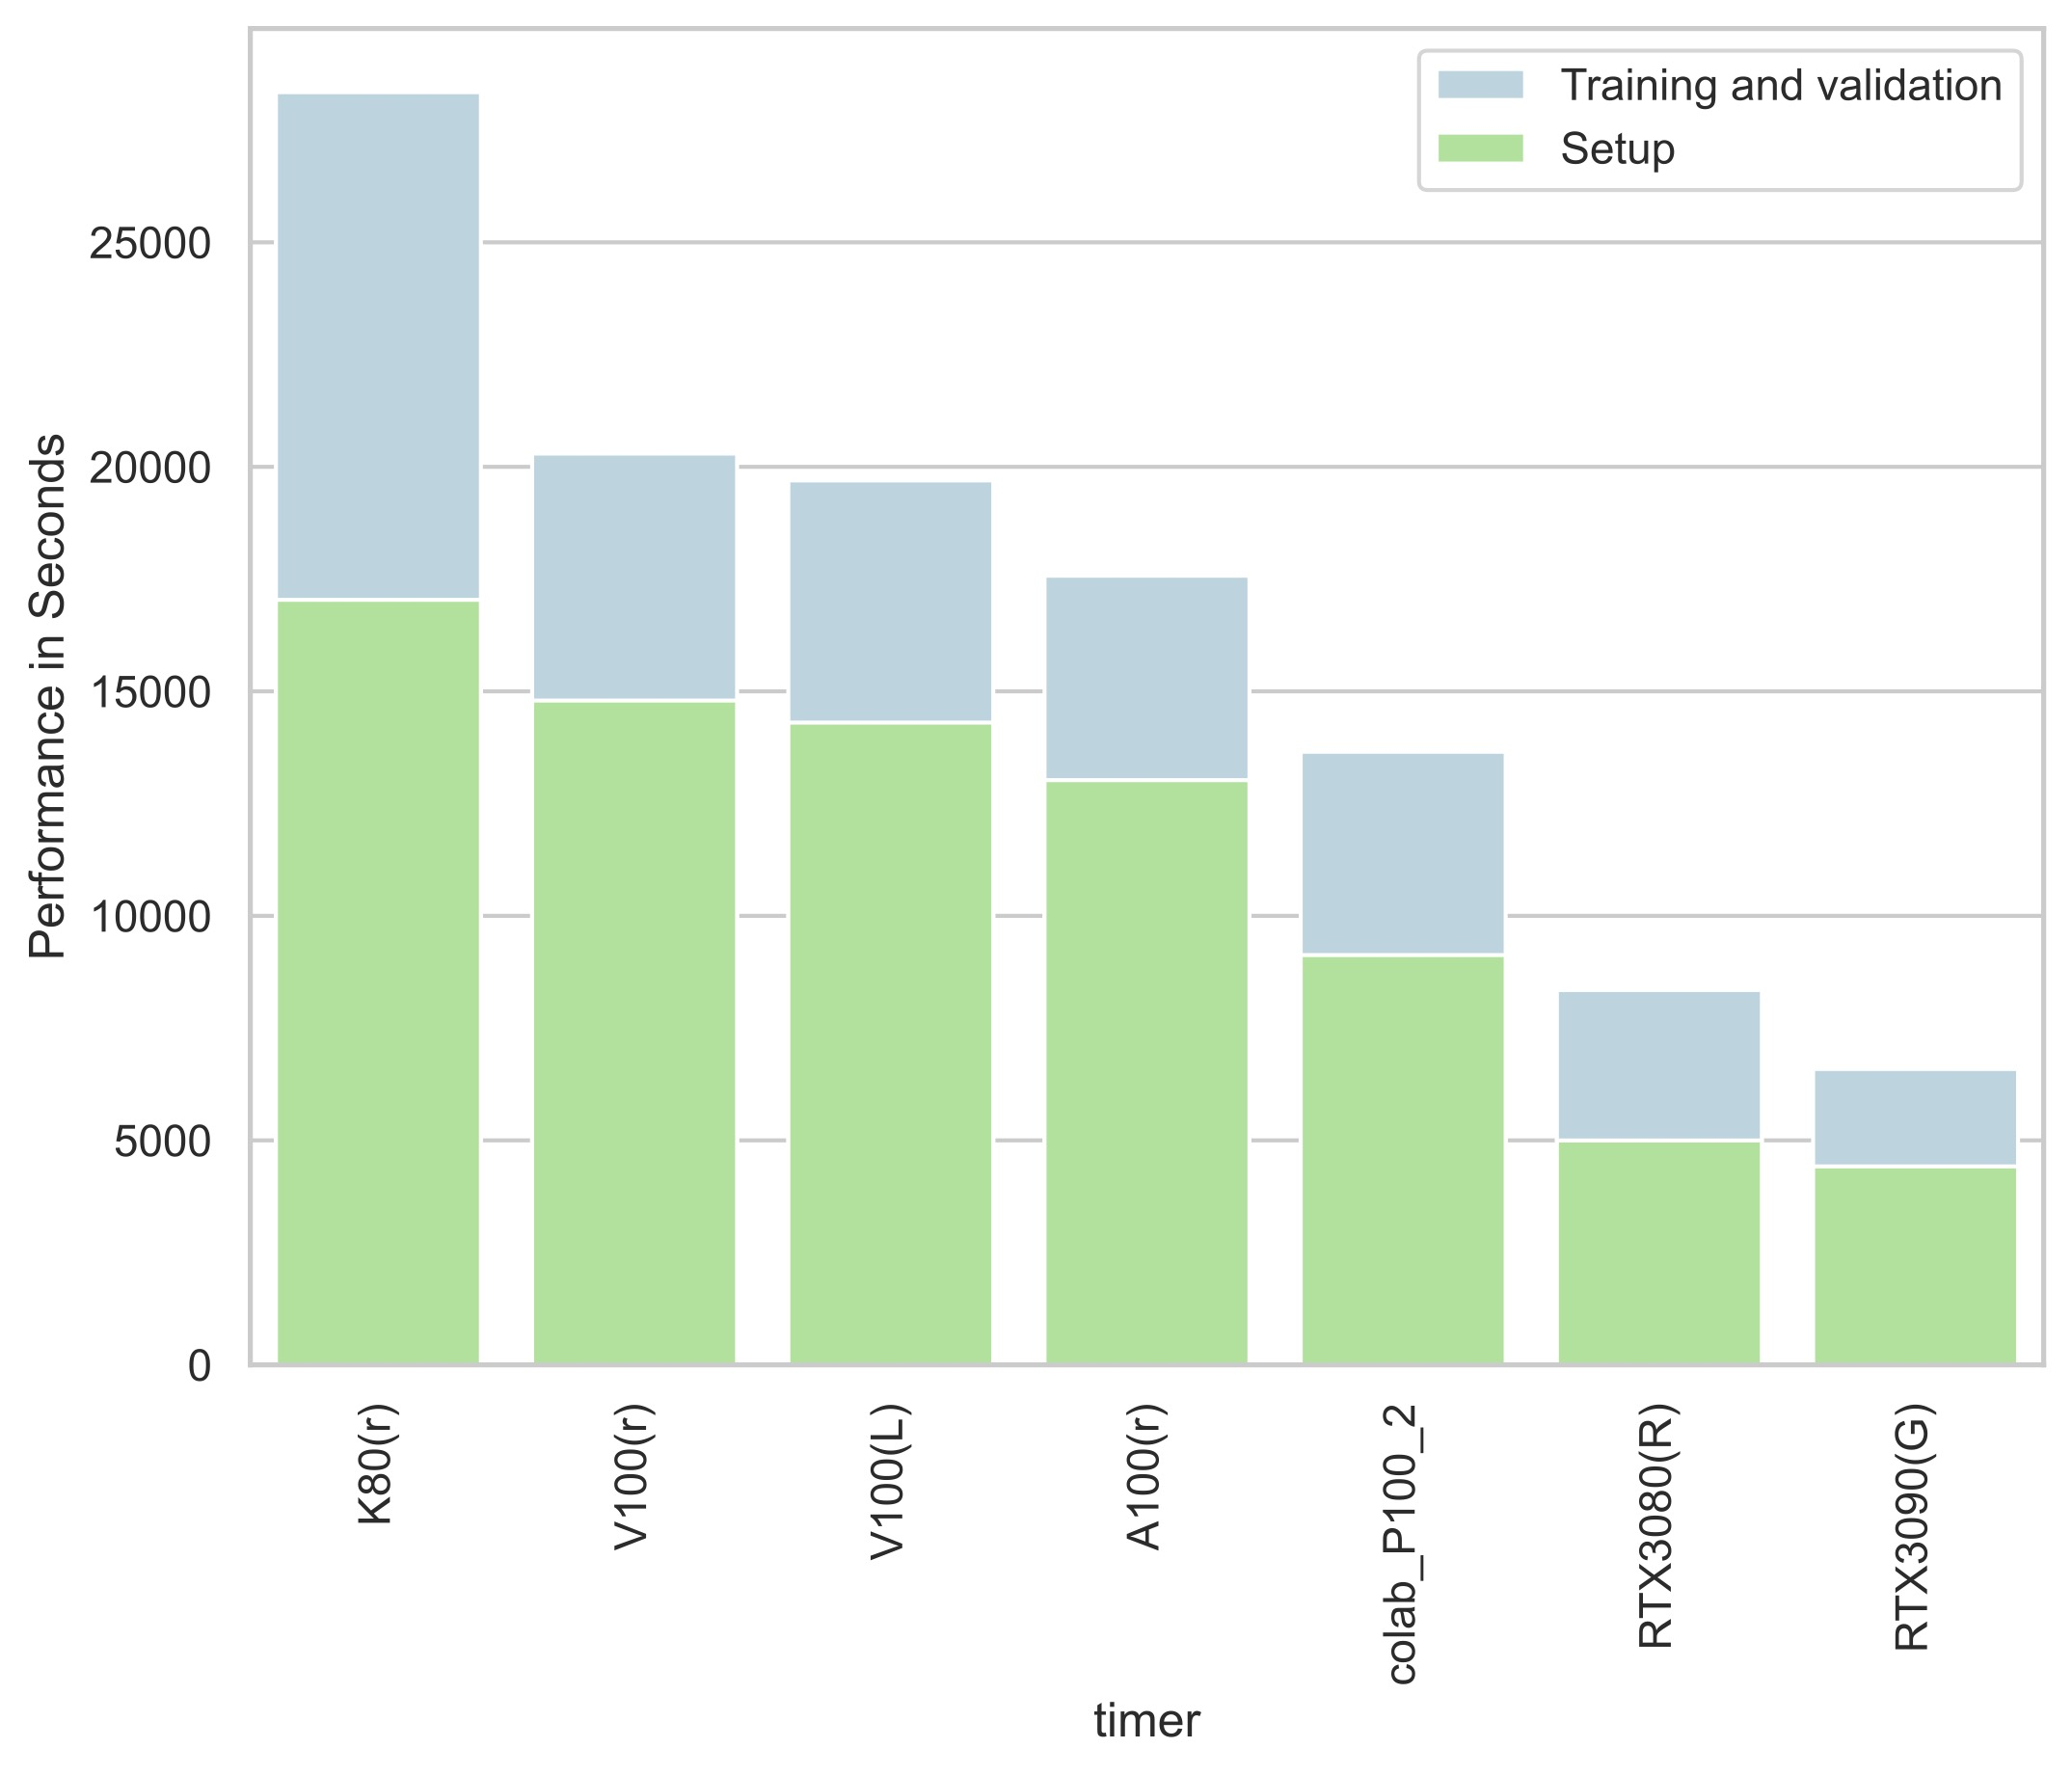
\includegraphics[width=0.75\columnwidth]{images/Graphics_Cards_BestFit_bar}

  {\bf (A)} Time of the best fit in seconds of performance measurements while using 2 epochs on various systems with different GPUs. The lower portion of each bar represents the setup time, while the upper portion represents the training and prediction time. The setup time is constant throughout the experiments, while with increasing number of epochs the training and prediction time will dominate. 
  
  
  \bigskip

  \centering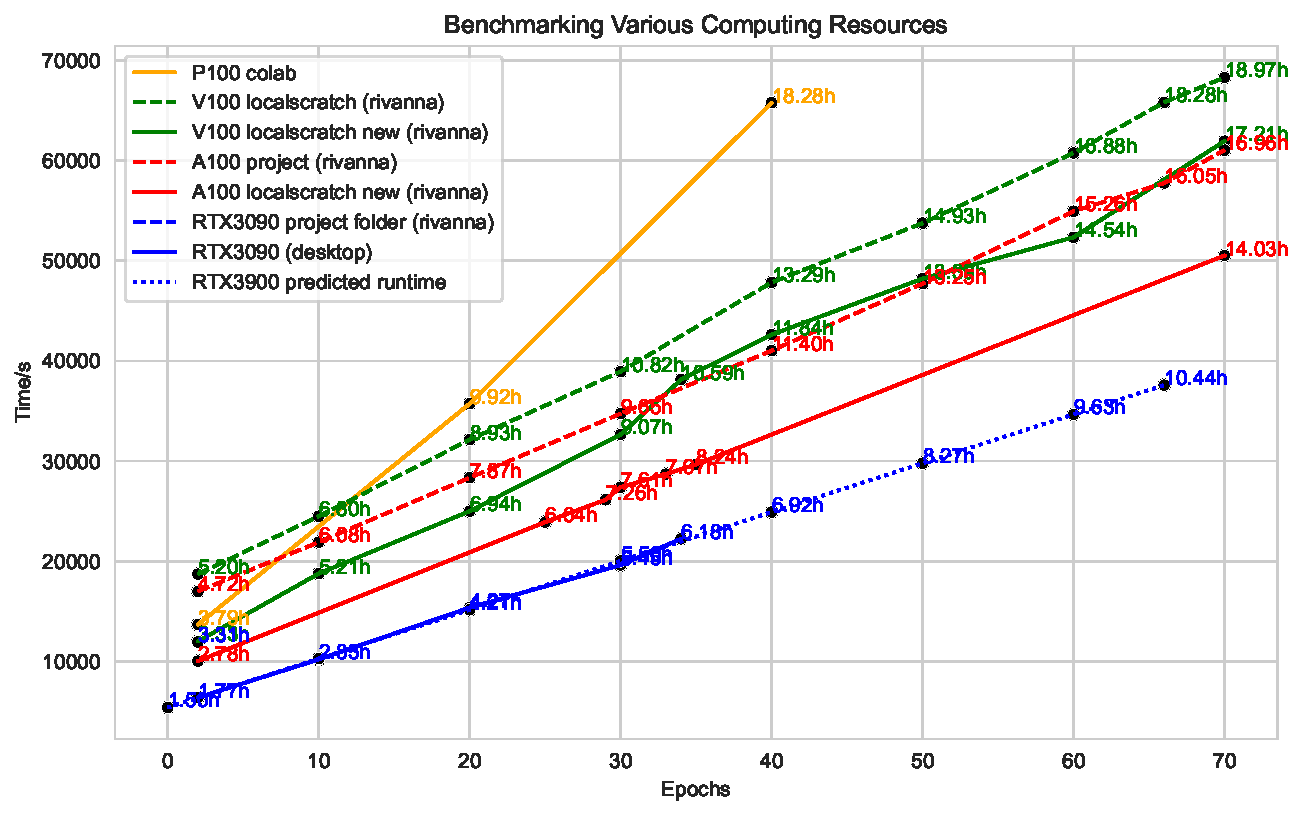
\includegraphics[width=0.9\columnwidth]{images/Benchmark_comp_resource_new}

  {\bf (B)} Time performance benchmark for various GPU cards on different systems and variations of epochs.
  
  
    
  \caption{Performance time measurements.}
  \label{fig:performance-projection}
\end{figure}

\begin{table}[htb]
    \caption{Runtime of the 2 epoch case in seconds}
    \label{tab:2-epoch-case}
    \begin{center}
    {\footnotesize              

          \begin{tabular}{|lrrrrr|}
            \hline
            {\bf Timer}             & {\bf RTX3090} & {\bf RTX3080} & {\bf A100 80GB} & {\bf V100}    & {\bf K80}     \\
                                    & Desktop & Laptop  & Rivanna & Rivanna & Rivanna \\
            \hline
            \hline
            Total             & 6589.4  & 8348.5  & 17574.8 & 20295.0 & 28343.3 \\
            Sampling location &  457.9  &  532.5  &  1227.0 &  1546.4 &  1779.6 \\
            Training          & 1103.2  & 2068.9  &  1373.0 &  1671.4 &  6967.3 \\
            Bestfit           & 4420.3  & 4997.1  & 13022.1 & 14795.1 & 17037.6 \\
            \hline
          \end{tabular}

    }
    \end{center}
\end{table}

For our next experiments, we need to distinguish the different phases of the application in more detail. We have augmented the code with timers that return information about the following phases:

\begin{itemize}
\item {\bf Total.} This shows the total runtime of the application and includes all additional phases mentioned here.
\item {\bf Initialize.} Time to initialize all variables and data and split data into train, validation, and test.
\item {\bf Sampling locations.} Time to sample time series data into 2-week batches.
\item {\bf Training or Model Fit.} Time to train the model and determine and save the best fit from all epochs.
\item {\bf Bestfit or Bestfit Prediction.} Time to find the best-fit model to calculate predictions.
\item {\bf Visualize.} Time to organize all predictions into an organized structure so the MSE and NNSE can be calculated and accuracy graphs can be identified.
\item {\bf Final Plots.} Time to gather data collected during model runtime and move to a permanent directory and process plots and graphs from data. Then, clean up data and close all unneeded processes.
\end{itemize}


\subsubsection{Accuracy Performance Benchmark}
\label{sec:perf-accuracy}

Since MLCommons Science Working Group's focus is improving an application’s accuracy, this next section reports on the accuracy of the earthquake application.

We observe that application loss for validation and training intersects at the 30-33 epoch value (see Figure~\ref{fig:loss}). We have also tested larger epoch runs up to 90 epochs. Our best accuracy values are found at our 90 epoch runs.

However, generally we can say that at the intersection point the model's performance on the validation set starts to degrade while its performance on the training set continues to improve. Hence, the  model is fitting the training data too well while at the same time not being able to generalize our validation data leading to overfitting. As the training loss continues to decrease with increased number of epochs after the intersection point, the model has become too complex and captures noise in the training data. This analysis provides an excelent opportunity for future benchmarking activities to deal with overfitting while considering techniques such as early stopping, regularization, the reduction of the medel complexity, reorganization of the data, cross-validation, and additional hyperparameter tuning. 

\begin{figure}[htb]
    \centering
    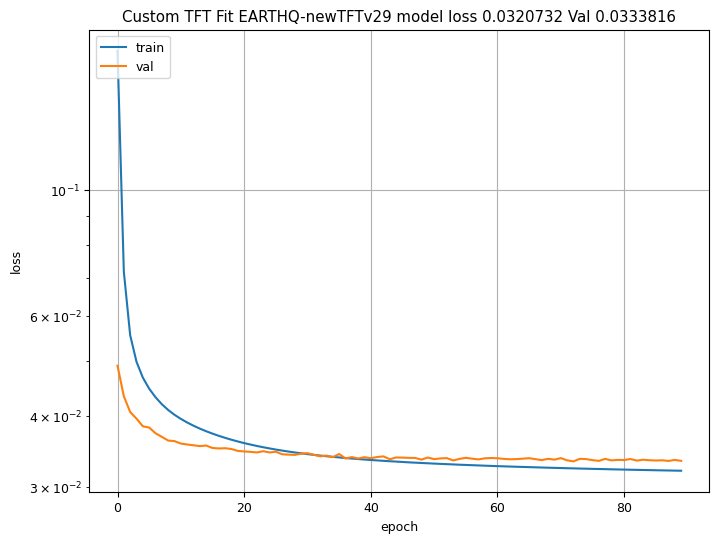
\includegraphics[width=0.70\columnwidth]{images/loss90.png}
    \caption{Loss comparision between training and validation data.}
    \label{fig:loss}
\end{figure}


\subsubsection{Prediction Parameters for Input and Prediction Data}

For the rest of the experiments, we have chosen different input and output vectors that are used as hyperparameters or prediction parameters. In the subsequent benchmark results, these groupings of data are used as part of the training to optimize their associated accuracy values. 

The data is grouped into 2 week periods. The model steps through each of these 2-week groupings and uses training data up to 1 year into the past from the current 2-week grouping. The model uses up to 1 year, $<=26$ data points, before the current 2-week grouping run on the model as training data. For example, the model is taking the first 2 weeks of January 2000, it would take $<=26$ 2-week groupings before that point as training data, so all of 1999 data would be 26 data points. Then it repeats this method with the next 2-week period in sequence so the 2-week grouping of weeks 3 and 4 of January 2000 and the training data would be the previous 26 2-week groupings from that point or the first 2 weeks of January 2000 and the previous 25 2 week groupings of 1999, all of 1999 data except first two weeks of 1999. It repeats this until all 2-week groupings are used in the model.

We have introduced a convenient nomenclature for the data input. This nomenclature uses the following rules that are applied to control how parameters are used as input and output data:

\begin{itemize}
  \item All data were grouped into 2-week periods.
  \item The term {\em Now} indicates the most recent rolling sequential date from the dataset, the Term {\em \#M} or {\em \#Y}    corresponds to the number of Months or Years prior to {\em Now} to use when sampling the data.
  \item An optional moving window is applied based on a range of    2-week grouping from the specified time frame.  For example,    2wk+26AVG is an abbreviation for performing the calculation over    26 groupings.  When not specified, only one observation is collected.
\end{itemize}



Applying these rules, a range of values is notated by first specifying a 2-week grouping and then the number of observations to include. For example, a value of {\em 1Y 2wk+26AVG} is one year from the 2-week grouping the model is currently on; the rolling training group is run on the dataset, taking 26 2-week groupings from that date. Another example is the value of {\em 1 Year Back}, which is a single 2-week occurrence one year ago from the rolling training group. Another example is {\em Now 2wk+7AVG}, which is 7 2-week groups from the rolling training group.


\subsubsection{Competitive Accuracy Benchmarks}

Next, we summarize the competitive accuracy benchmark where we use the nomenclature for the input and output hyperparameters defining the time period used for the training and validation.  To simplify our presentation, we have decided to use epoch values 2, 30, 70, and 90 for this paper's experiments. We took all results and sorted them for training and validation separately by the accuracy values. This leads to a ranking of the experiments by accuracy. In Table \ref{tab:ranking-accuracy} we present the top 20 accuracy values, while in Figure \ref{fig:NNSE-comparison-a100}A and \ref{fig:NNSE-comparison-a100}B we created a histogram showcasing how many accuracy values fall into a certain bucket over all experiments for training and validation.

From the table, we see that we achieve the best results using the parameters (epoch=90, Next Year Back). From the histogram, we see that the best results stem mostly from 90 epochs.

Hence, although we are mostly interested in identifying the best accuracy value, it is also advantageous to reflect that data places the 90 epoch case above the other values, generally leading to better results (see Figure \ref{fig:NNSE-comparison-a100}A) for training.


    \begin{table}[htb]
      \caption{Ranking of the top 20 accuracy values.}\
      \label{tab:ranking-accuracy}
    
        {\bf (A)} The top 20 {\em average} accuracy values based on hyperparameters with 2, 30, 70, and 90 epochs.\

\renewcommand{\arraystretch}{1.2}
      \begin{center}
        {\footnotesize
    \begin{tabular}{|r|r|r|l| |r|r|r|l|}
      \hline
     \multicolumn{4}{|c||}{\bf \textcolor{red}{Training}}  & \multicolumn{4}{c|}{\bf \textcolor{blue}{Validation}}  \\
    {\bf Rank} &  {\bf NNSE} &  {\bf Epoch} & {\bf Prediction Parameter} & Rank & {\bf NNSE} &  {\bf Epoch} & {\bf Prediction Parameter}\\
    \hline
    \hline
        \textcolor{red}{1}  &  \textcolor{red}{0.937} &     \textcolor{red}{90} &  \textcolor{red}{Next Year Back} &  1 & \textcolor{blue}{0.937} &     \textcolor{blue}{90} &  \textcolor{blue}{Next Year Back} \\
    2  &  0.933 &     90 &      Next Year Back &  2 & 0.931 &     90 &      Next Year Back \\
3  &  0.932 &     70 &      Next Year Back &  3 & 0.931 &     70 &      Next Year Back \\
4  &  0.928 &     90 &      Next Year Back &  4 & 0.927 &     90 &      Next Year Back \\
5  &  0.926 &     90 &      Next Year Back &  5 & 0.925 &     90 &      Next Year Back \\
6  &  0.919 &     30 &      Next Year Back &  6 & 0.917 &     30 &      Next Year Back \\
7  &  0.916 &     70 &      Next Year Back &  7 & 0.915 &     70 &      Next Year Back \\
8  &  0.916 &     70 &      Next Year Back &  8 & 0.915 &     70 &      Next Year Back \\
9  &  0.911 &     90 &  Next 6 Months Back &  9 & 0.913 &     90 &  Next 6 Months Back \\
10  &  0.907 &     30 &      Next Year Back &  10 & 0.906 &     30 &      Next Year Back \\
11  &  0.906 &     30 &      Next Year Back &  11 & 0.904 &     90 &  Next 6 Months Back \\
12  &  0.902 &     90 &  Next 6 Months Back &  12 & 0.904 &     30 &      Next Year Back \\
13  &  0.899 &     70 &  Next 6 Months Back &  13 & 0.901 &     90 &  Next 6 Months Back \\
14  &  0.899 &     30 &      Next Year Back &  14 & 0.899 &     70 &  Next 6 Months Back \\
15  &  0.899 &     90 &  Next 6 Months Back &  15 & 0.899 &     70 &  Next 6 Months Back \\
16  &  0.897 &     70 &  Next 6 Months Back &  16 & 0.896 &     30 &      Next Year Back \\
17  &  0.895 &     30 &      Next Year Back &  17 & 0.894 &     30 &      Next Year Back \\
18  &  0.89 &     70 &  Next 6 Months Back &  18 & 0.893 &     70 &  Next 6 Months Back \\
19  &  0.886 &     90 &  Next 6 Months Back &  19 & 0.888 &     90 &  Next 6 Months Back \\
20  &  0.882 &     30 &  Next 6 Months Back &  20 & 0.884 &     30 &  Next 6 Months Back \\

        \hline
        \end{tabular}
        }
        \end{center}
        
        {\bf (B)} The top 20 {\em summed} accuracy values based on hyperparameters with 2, 30, 70, and 90 epochs.

      \renewcommand{\arraystretch}{1.2}
      \begin{center}
        {\footnotesize
    \begin{tabular}{|r|r|r|l| |r|r|r|l|}
      \hline
     \multicolumn{4}{|c||}{\bf \textcolor{red}{Training}}  & \multicolumn{4}{c|}{\bf \textcolor{blue}{Validation}}  \\
    {\bf Rank} &  {\bf NNSE} &  {\bf Epoch} & {\bf Prediction Parameter} & Rank & {\bf NNSE} &  {\bf Epoch} & {\bf Prediction Parameter}\\
    \hline
    \hline
        \textcolor{red}{1}  &  \textcolor{red}{0.99} &     \textcolor{red}{90} &  \textcolor{red}{Next 6 Months Back} &  1 & \textcolor{blue}{0.983} &     \textcolor{blue}{90} &  \textcolor{blue}{Next 6 Months Back} \\
    2  &  0.988 &     90 &  Next 6 Months Back & 2  & 0.98 &     90 &  Next 6 Months Back \\
3  &  0.985 &     30 &  Next 6 Months Back &   3  & 0.976 &     90 &      Next Year Back \\
4  &  0.984 &     30 &      Next Year Back &   4  & 0.975 &     30 &      Next Year Back \\
5  &  0.983 &     70 &  Next 3 Months Back &   5  & 0.974 &     30 &  Next 6 Months Back \\
6  &  0.982 &     90 &      Next Year Back &   6  & 0.974 &     70 &  Next 3 Months Back \\
7  &  0.981 &     30 &  Next 6 Months Back &   7  & 0.973 &     30 &  Next 6 Months Back \\
8  &  0.979 &     30 &  Next 3 Months Back &   8  & 0.971 &     30 &  Next 3 Months Back \\
9  &  0.979 &     30 &  Next 3 Months Back &   9  & 0.97 &     30 &  Next 3 Months Back \\
10  &  0.977 &     30 &      Next Year Back &  10 & 0.97 &     30 &      Next Year Back \\
11  &  0.976 &     30 &  Next 3 Months Back &  11 & 0.968 &     30 &  Next 3 Months Back \\
12  &  0.973 &     30 &  Next 3 Months Back &  12 & 0.966 &     90 &  Next 3 Months Back \\
13  &  0.971 &     90 &  Next 3 Months Back &  13 & 0.965 &     70 &  Next 3 Months Back \\
14  &  0.971 &     70 &  Next 3 Months Back &  14 & 0.965 &     90 &  Next 3 Months Back \\
15  &  0.97 &     90 &  Next 3 Months Back &   15 & 0.964 &     30 &  Next 3 Months Back \\
16  &  0.967 &     90 &  Next 3 Months Back &  16 & 0.962 &     90 &  Next 3 Months Back \\
17  &  0.958 &     90 &      Next Year Back &  17 & 0.954 &     90 &      Next Year Back \\
18  &  0.956 &     90 &     Year Back 2wk+7 &  18 & 0.942 &     30 &  Next 6 Months Back \\
19  &  0.955 &     90 &     Year Back 2wk+7 &  19 & 0.942 &     90 &  Next 6 Months Back \\
20  &  0.955 &     30 &     Year Back 2wk+7 &  20 & 0.939 &     70 &  Next 6 Months Back \\

        \hline
        \end{tabular}
        }
        \end{center}
        
        \end{table}

\begin{comment}

\begin{table}[htb]
      \caption{Ranking of the top 20 accuracy values sorted by descending training NNSE datapoints.}\
      \label{tab:ranking-accuracy}
    
        {\bf (A)} The top 20 {\em average} accuracy values based on hyperparameters with 2, 30, 70, and 90 epochs.\

      \renewcommand{\arraystretch}{1.2}
      \begin{center}
        {\footnotesize
    \begin{tabular}{|l||r|r|l|r|r|l|}
      \hline
     &   \multicolumn{3}{c|}{\bf \textcolor{red}{Training}}  & \multicolumn{3}{c|}{\bf \textcolor{blue}{Validation}}  \\
    {\bf Rank} &  {\bf NNSE} &  {\bf Epoch} & {\bf Prediction Parameter} & {\bf NNSE} &  {\bf Epoch} & {\bf Prediction Parameter}\\
    \hline
    \hline
        \textcolor{red}{1}  &  \textcolor{red}{0.937} &     \textcolor{red}{90} &  \textcolor{red}{Next Year Back} &  \textcolor{blue}{0.937} &     \textcolor{blue}{90} &  \textcolor{blue}{Next Year Back} \\
    2  &  0.933 &     90 &      Next Year Back &  0.931 &     90 &      Next Year Back \\
3  &  0.932 &     70 &      Next Year Back &  0.931 &     70 &      Next Year Back \\
4  &  0.928 &     90 &      Next Year Back &  0.927 &     90 &      Next Year Back \\
5  &  0.926 &     90 &      Next Year Back &  0.925 &     90 &      Next Year Back \\
6  &  0.919 &     30 &      Next Year Back &  0.917 &     30 &      Next Year Back \\
7  &  0.916 &     70 &      Next Year Back &  0.915 &     70 &      Next Year Back \\
8  &  0.916 &     70 &      Next Year Back &  0.915 &     70 &      Next Year Back \\
9  &  0.911 &     90 &  Next 6 Months Back &  0.913 &     90 &  Next 6 Months Back \\
10  &  0.907 &     30 &      Next Year Back &  0.906 &     30 &      Next Year Back \\
11  &  0.906 &     30 &      Next Year Back &  0.904 &     30 &      Next Year Back \\
12  &  0.902 &     90 &  Next 6 Months Back &  0.904 &     90 &  Next 6 Months Back \\
13  &  0.899 &     70 &  Next 6 Months Back &  0.899 &     70 &  Next 6 Months Back \\
14  &  0.899 &     30 &      Next Year Back &  0.896 &     30 &      Next Year Back \\
15  &  0.899 &     90 &  Next 6 Months Back &  0.901 &     90 &  Next 6 Months Back \\
16  &  0.897 &     70 &  Next 6 Months Back &  0.899 &     70 &  Next 6 Months Back \\
17  &  0.895 &     30 &      Next Year Back &  0.894 &     30 &      Next Year Back \\
18  &  0.89 &     70 &  Next 6 Months Back &  0.893 &     70 &  Next 6 Months Back \\
19  &  0.886 &     90 &  Next 6 Months Back &  0.888 &     90 &  Next 6 Months Back \\
20  &  0.882 &     30 &  Next 6 Months Back &  0.884 &     30 &  Next 6 Months Back \\

        \hline
        \end{tabular}
        }
        \end{center}
        
        {\bf (B)} The top 20 {\em summed} accuracy values based on hyperparameters with 2, 30, 70, and 90 epochs.\

      \renewcommand{\arraystretch}{1.2}
      \begin{center}
        {\footnotesize
    \begin{tabular}{|l||r|r|l|r|r|l|}
      \hline
     &   \multicolumn{3}{c|}{\bf \textcolor{red}{Training}}  & \multicolumn{3}{c|}{\bf \textcolor{blue}{Validation}}  \\
    {\bf Rank} &  {\bf NNSE} &  {\bf Epoch} & {\bf Prediction Parameter} & {\bf NNSE} &  {\bf Epoch} & {\bf Prediction Parameter}\\
    \hline
    \hline
        \textcolor{red}{1}  &  \textcolor{red}{0.99} &     \textcolor{red}{90} &  \textcolor{red}{Next 6 Months Back} &  \textcolor{blue}{0.983} &     \textcolor{blue}{90} &  \textcolor{blue}{Next 6 Months Back} \\
    2  &  0.988 &     90 &  Next 6 Months Back &  0.98 &     90 &  Next 6 Months Back \\
3  &  0.985 &     30 &  Next 6 Months Back &  0.974 &     30 &  Next 6 Months Back \\
4  &  0.984 &     30 &      Next Year Back &  0.975 &     30 &      Next Year Back \\
5  &  0.983 &     70 &  Next 3 Months Back &  0.974 &     70 &  Next 3 Months Back \\
6  &  0.982 &     90 &      Next Year Back &  0.976 &     90 &      Next Year Back \\
7  &  0.981 &     30 &  Next 6 Months Back &  0.973 &     30 &  Next 6 Months Back \\
8  &  0.979 &     30 &  Next 3 Months Back &  0.968 &     30 &  Next 3 Months Back \\
9  &  0.979 &     30 &  Next 3 Months Back &  0.971 &     30 &  Next 3 Months Back \\
10  &  0.977 &     30 &      Next Year Back &  0.97 &     30 &      Next Year Back \\
11  &  0.976 &     30 &  Next 3 Months Back &  0.97 &     30 &  Next 3 Months Back \\
12  &  0.973 &     30 &  Next 3 Months Back &  0.964 &     30 &  Next 3 Months Back \\
13  &  0.971 &     90 &  Next 3 Months Back &  0.965 &     90 &  Next 3 Months Back \\
14  &  0.971 &     70 &  Next 3 Months Back &  0.965 &     70 &  Next 3 Months Back \\
15  &  0.97 &     90 &  Next 3 Months Back &  0.966 &     90 &  Next 3 Months Back \\
16  &  0.967 &     90 &  Next 3 Months Back &  0.962 &     90 &  Next 3 Months Back \\
17  &  0.958 &     90 &      Next Year Back &  0.954 &     90 &      Next Year Back \\
18  &  0.956 &     90 &     Year Back 2wk+7 &  0.937 &     90 &     Year Back 2wk+7 \\
19  &  0.955 &     90 &     Year Back 2wk+7 &  0.937 &     90 &     Year Back 2wk+7 \\
20  &  0.955 &     30 &     Year Back 2wk+7 &  0.935 &     30 &     Year Back 2wk+7 \\

        \hline
        \end{tabular}
        }
        \end{center}
        
\end{table}

\end{comment}

        
To identify more details about the most accurate results and the prediction parameters (hyperparameters) used to create them, we have plotted the accuracy values in Figure~\ref{fig:performance-projection}C and \ref{fig:performance-projection}D.

Here we have sorted the hyperparameters by the accuracy values for the validation where the best accuracy for each hyperparameter is identified and sorted in increasing fashion. We have then taken the same order of the hyperparameters and applied to the training.  The diagrams include the minimum and maximum accuracy values for a hyperparameter found using 2, 30, 70, and 90 as epochs, while the experiment has been repeated 5 times. The average for each accuracy for a given epoch is shown. Additionally, the confidence interval for each epoch is added as a highlighted area.

The best average value for the hyperparameter {\em Next Year Back} is 0.937 for training and 0.937 for validation (see Table~\ref{tab:ranking-accuracy}).

Not only did we find that the best epoch for accuracy is 90, but the best hyperparameters are {\em Next Year Back} for average NNSE and {\em Next 6 Months Back} for summed NNSE, meaning according to our nomenclature the previous year and 6 months of observation readings from the current rolling training group is used as training data support our model.

Although we see on average better accuracy results with 30 epochs, the best accuracy values we still have seen with 90 epochs. This indicates that we have a higher variation of the results in the 90 epoch case. However, as we are competing for the best value and not the average value this variation has an advantage and we do not as easily get stuck in a local minima.

One other observation we can make is that the training NNSE value is higher than that of validation. This leads us to believe that the input data may be incomplete to train the model more accurately, or the input data needs to be differently structured to have a higher validation accuracy value.  Hence, although this work is a good starting point, we believe there is significant room for improvement.

We can make similar observations when looking at the summed accuracy values. However here we see that more of the best accuracy values are retrieved when using 90 epochs.  We see in the average and summed accuracy that the best 20 values have been created with the prediction parameters of {\em Next Year Back}, {\em Next 6 Month Back}, and {\em
  Next 3 Month Back}. The average shows a more uniform distribution of
these parameters in the top 20 than the summed NNSE values (see
Figure~\ref{fig:NNSE-comparison-a100-summed}).

As we see further educational opportunities can be derived from analyzing different prediction parameters, and different input data distributions.

\begin{figure}[p]

  \begin{center}
       \begin{minipage}[t]{0.49\textwidth}
        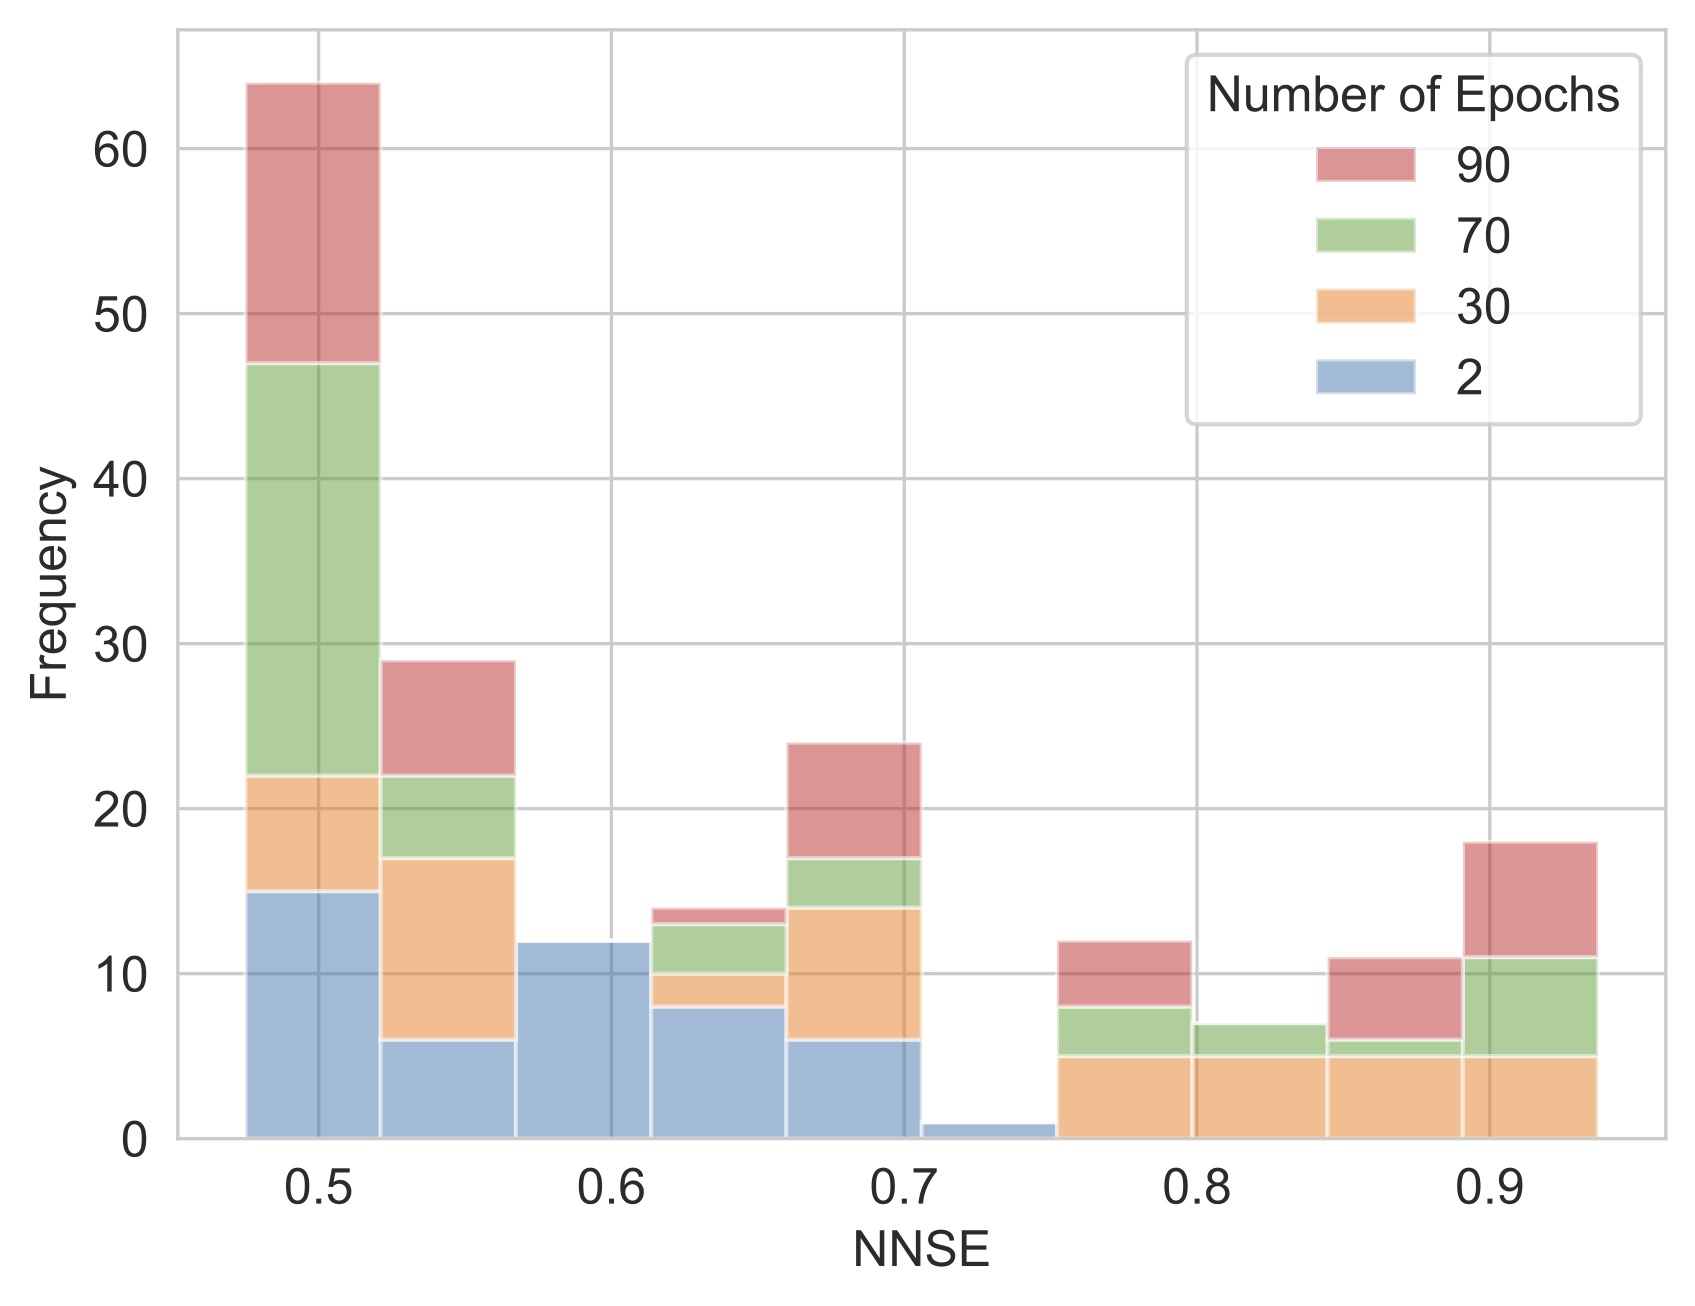
\includegraphics[width=1.0\linewidth]{images/frequency_nnse_histogram_stacked_df_training}
        {\bf (A)} Histogram of the average accuracy values for every epoch over all experiments for training.
     \end{minipage}
  \ \
     \begin{minipage}[t]{0.49\textwidth}
        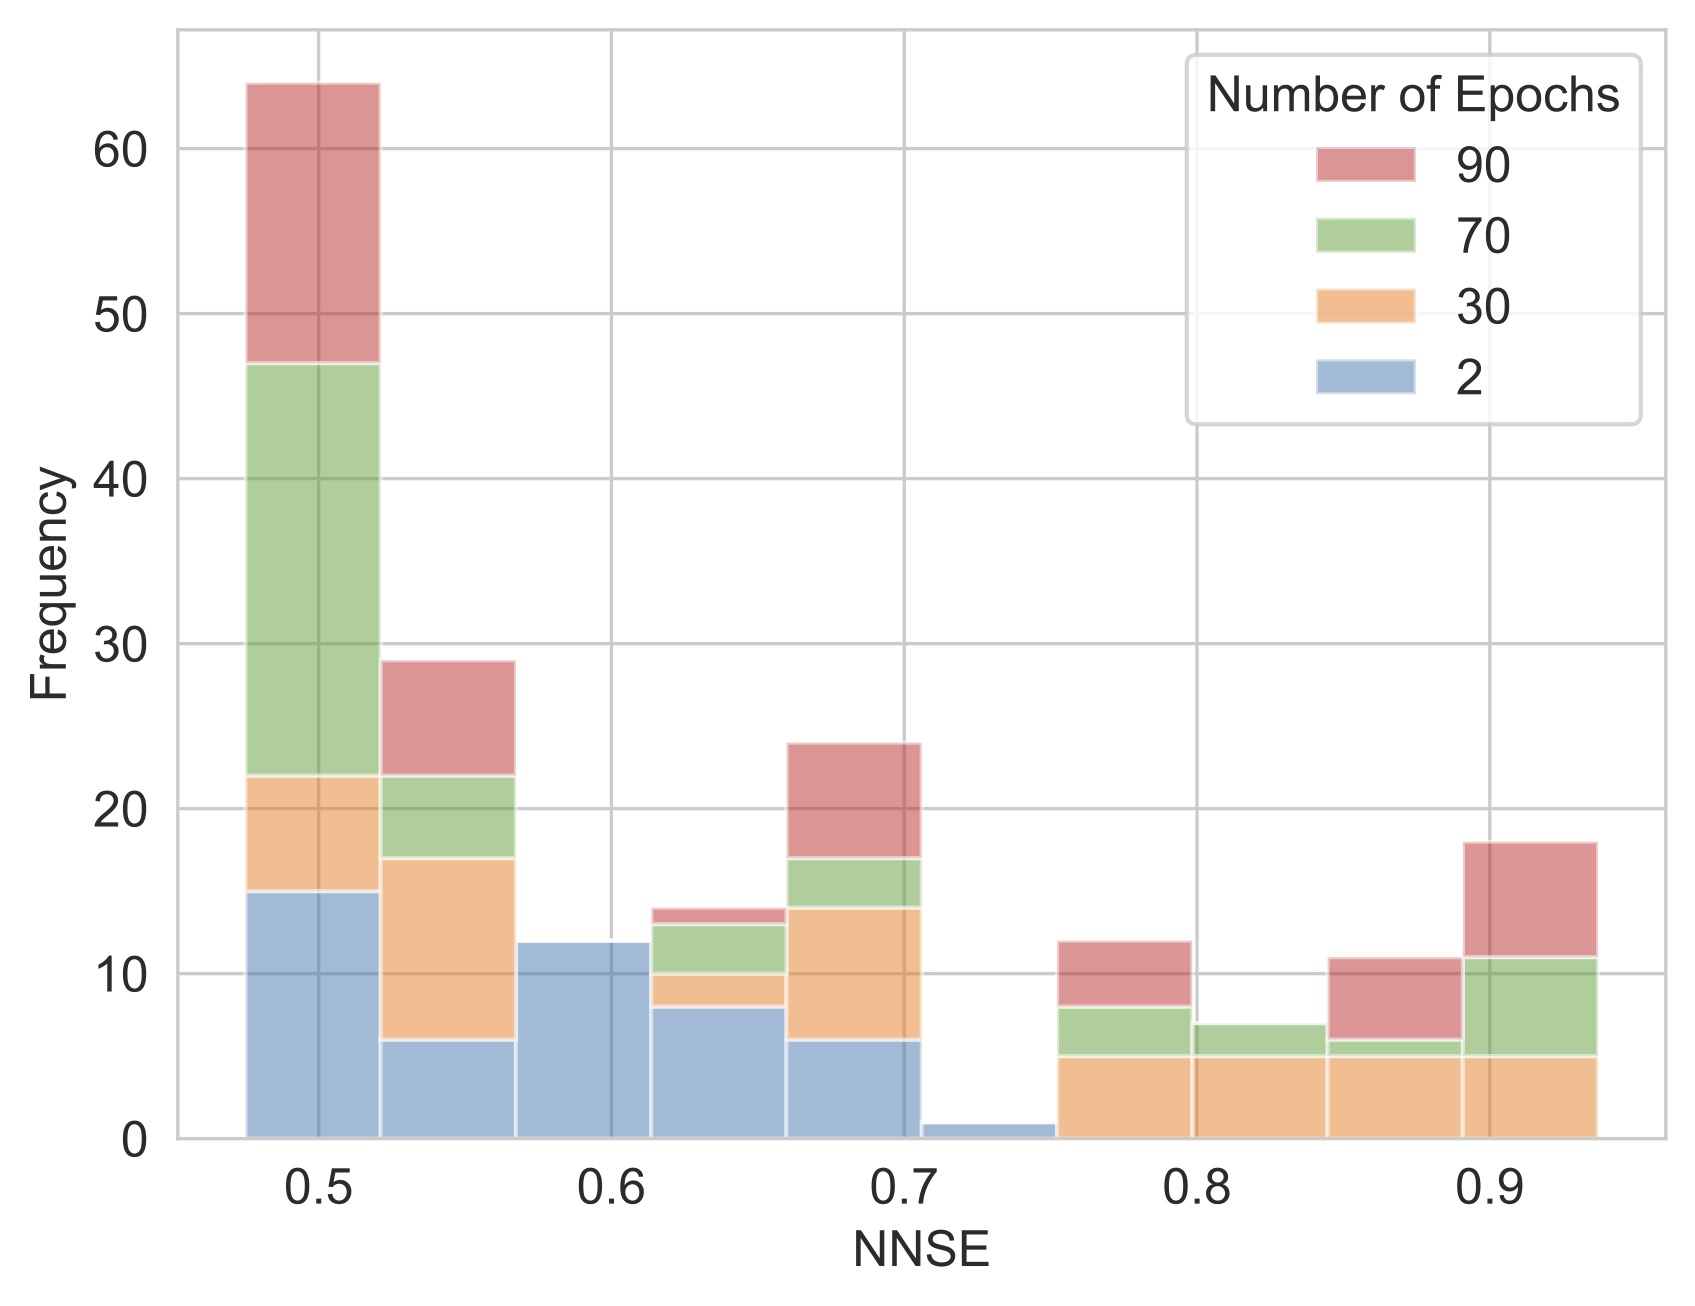
\includegraphics[width=1.0\linewidth]{images/frequency_nnse_histogram_stacked_df_validation}
        {\bf (B)} Histogram of the average accuracy values for every epoch over all experiments for validation.
     \end{minipage}
  \ \
     \begin{minipage}[t]{0.49\textwidth}
        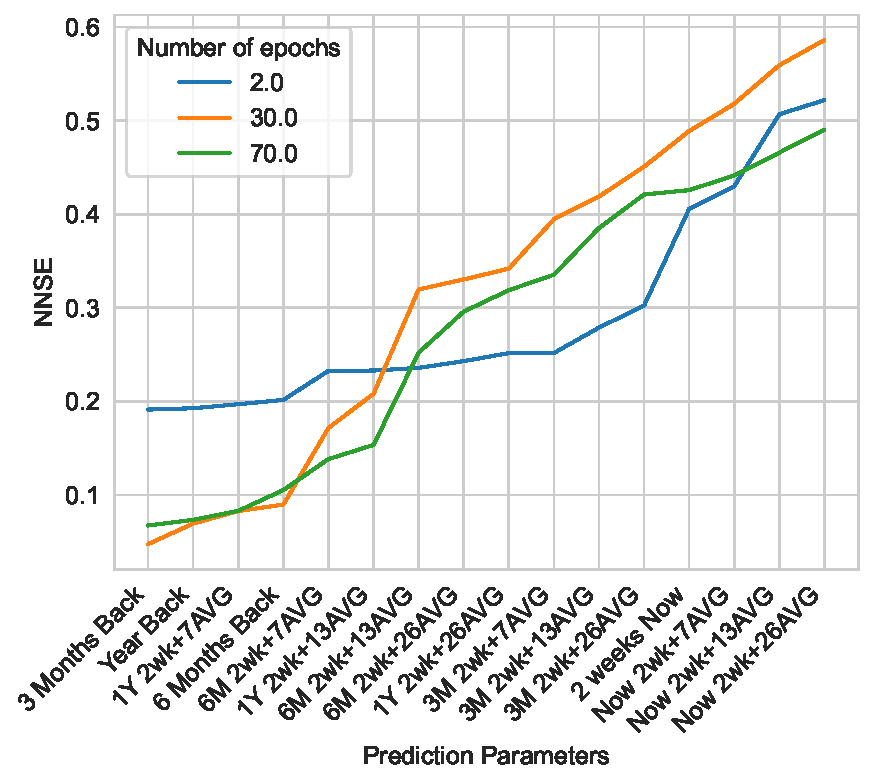
\includegraphics[width=1.0\linewidth]{images/NNSE-all-epochs-training}
        {\bf (C)} Average accuracy values over all experiments for training sorted by best training values.
     \end{minipage}
  \ \
     \begin{minipage}[t]{0.49\textwidth}
        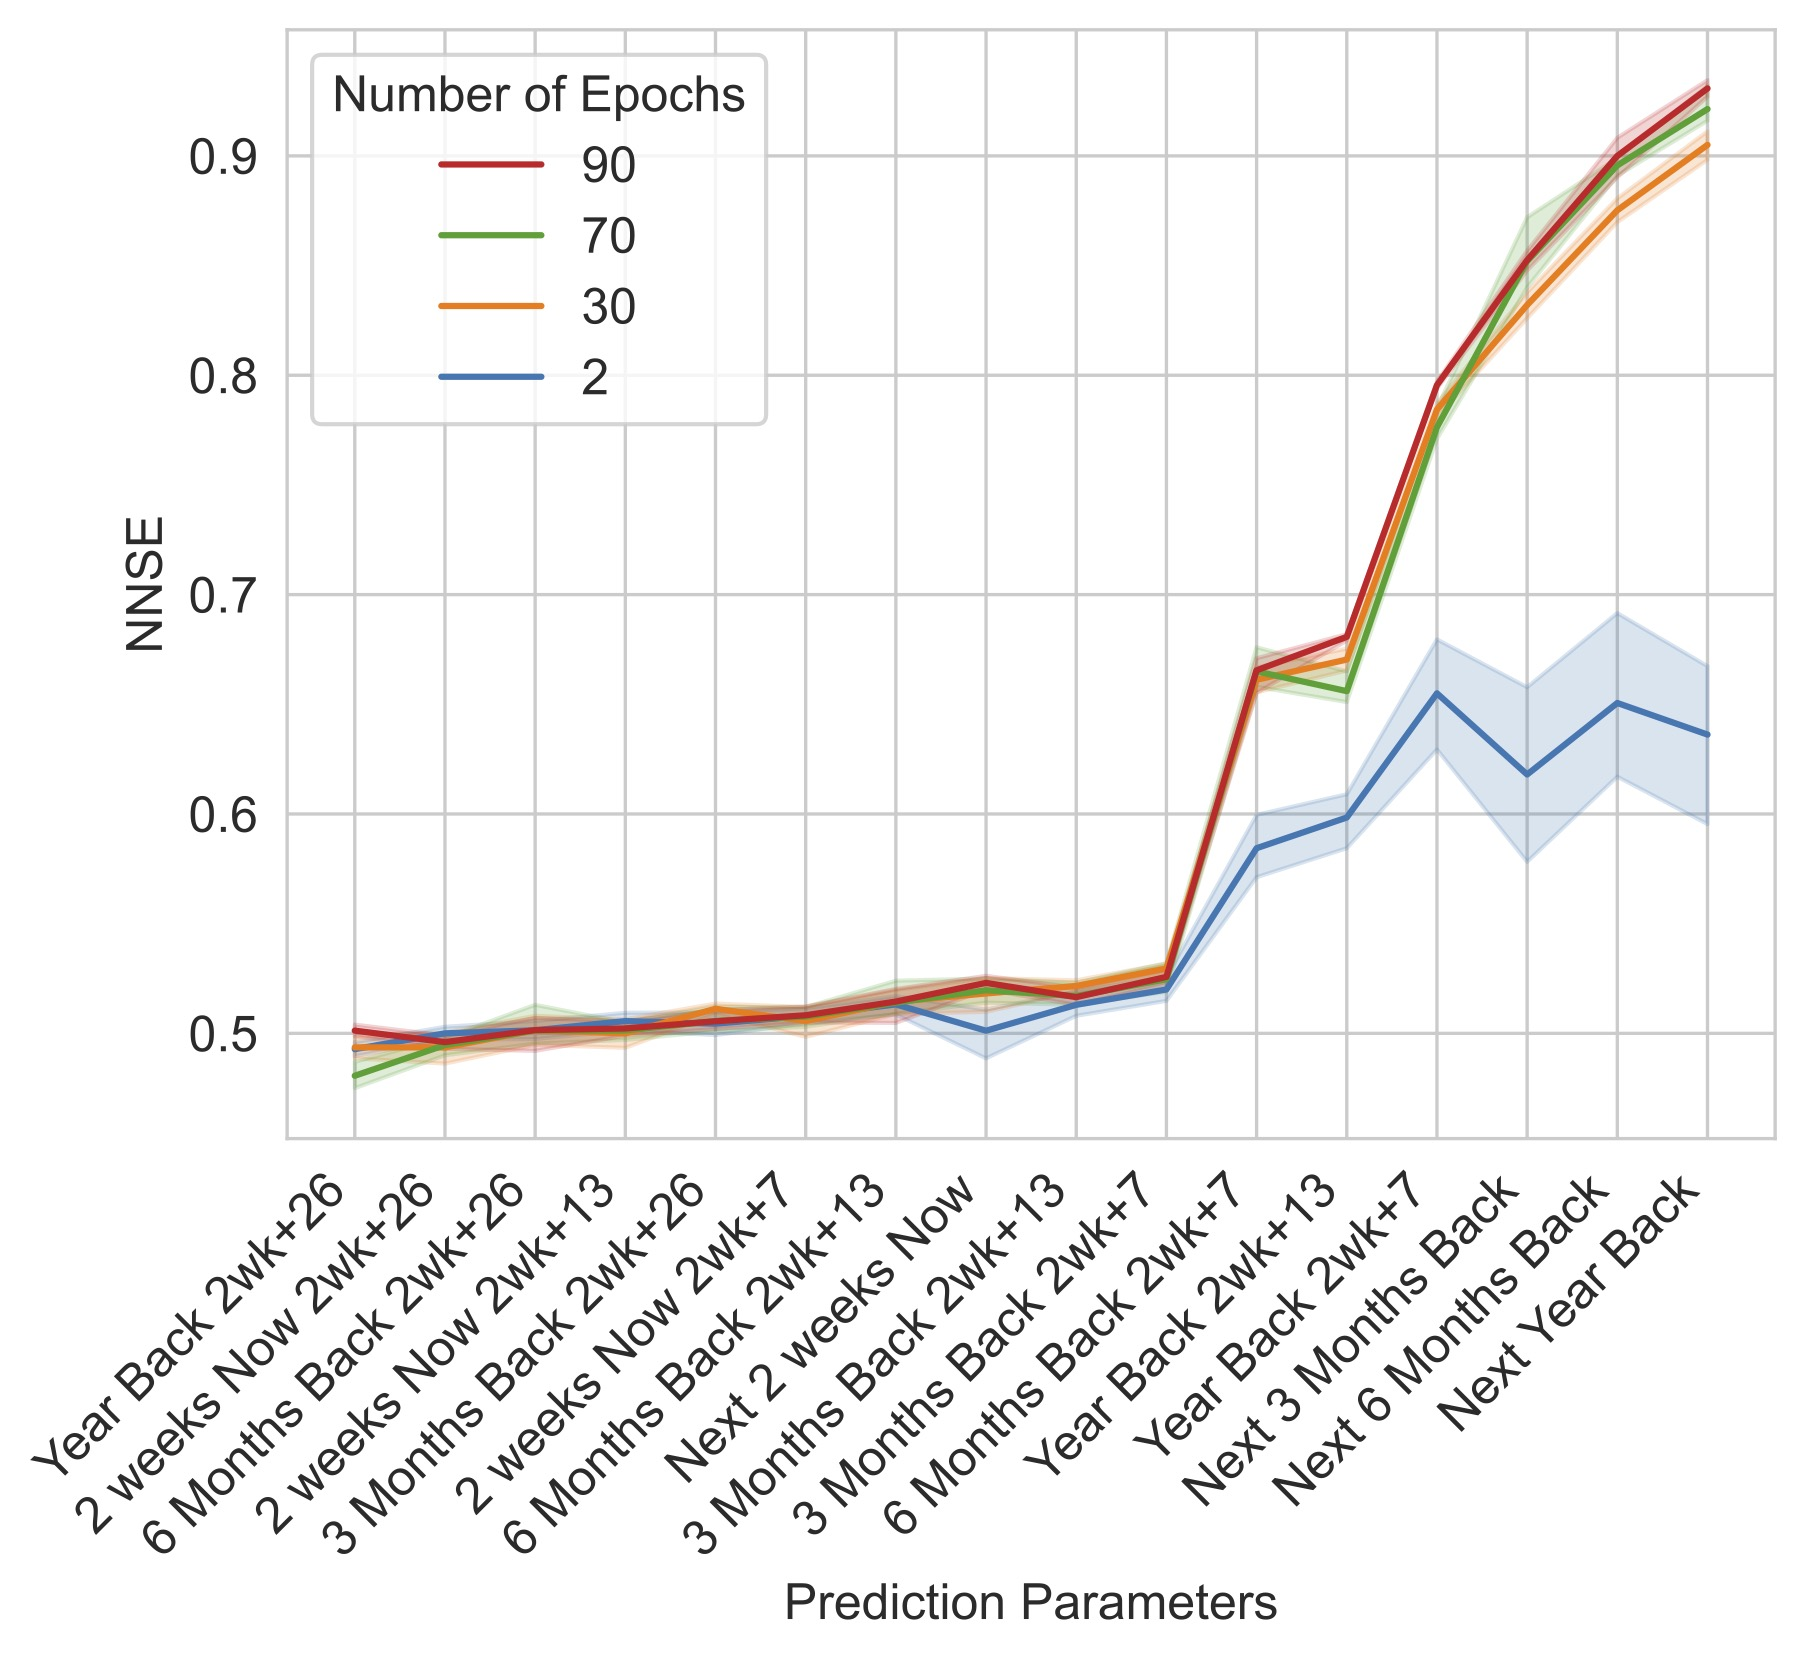
\includegraphics[width=1.0\linewidth]{images/NNSE-all-epochs-validation}
        {\bf (D)} Average accuracy values over all experiments for validation sorted by best validation values.
     \end{minipage}

  \end{center}

  \caption {Evaluation of the NNSE average accuracy for epochs 2, 30, 70, and 90.}
  \label{fig:NNSE-comparison-a100}

\end{figure}



\begin{figure}[p]

  \begin{center}
       \begin{minipage}[t]{0.49\textwidth}
        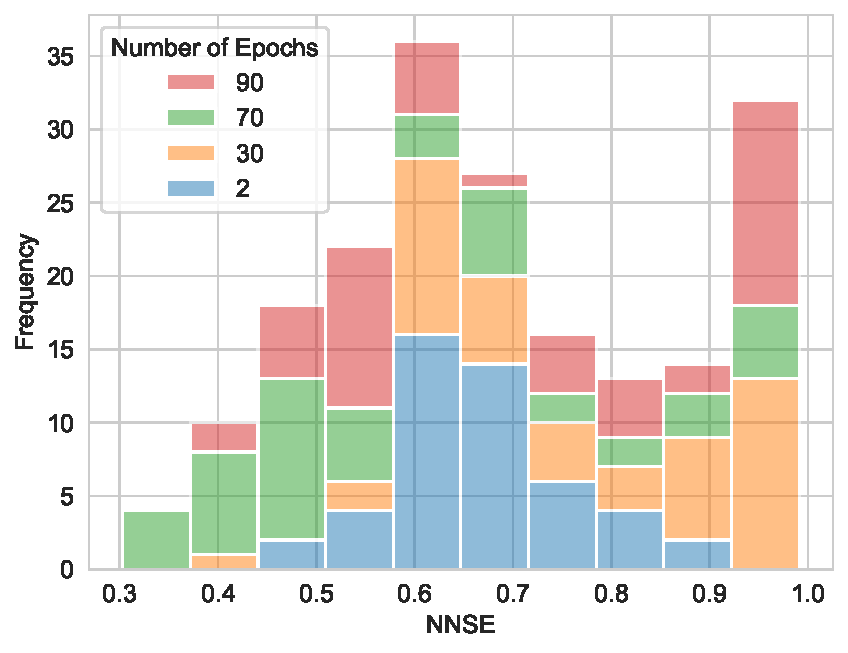
\includegraphics[width=1.0\linewidth]{images/frequency_nnse_histogram_stacked_df_training_summed}
        {\bf (A)} Histogram of the summed accuracy values for every epoch over all experiments for training.
     \end{minipage}
  \ \
     \begin{minipage}[t]{0.49\textwidth}
        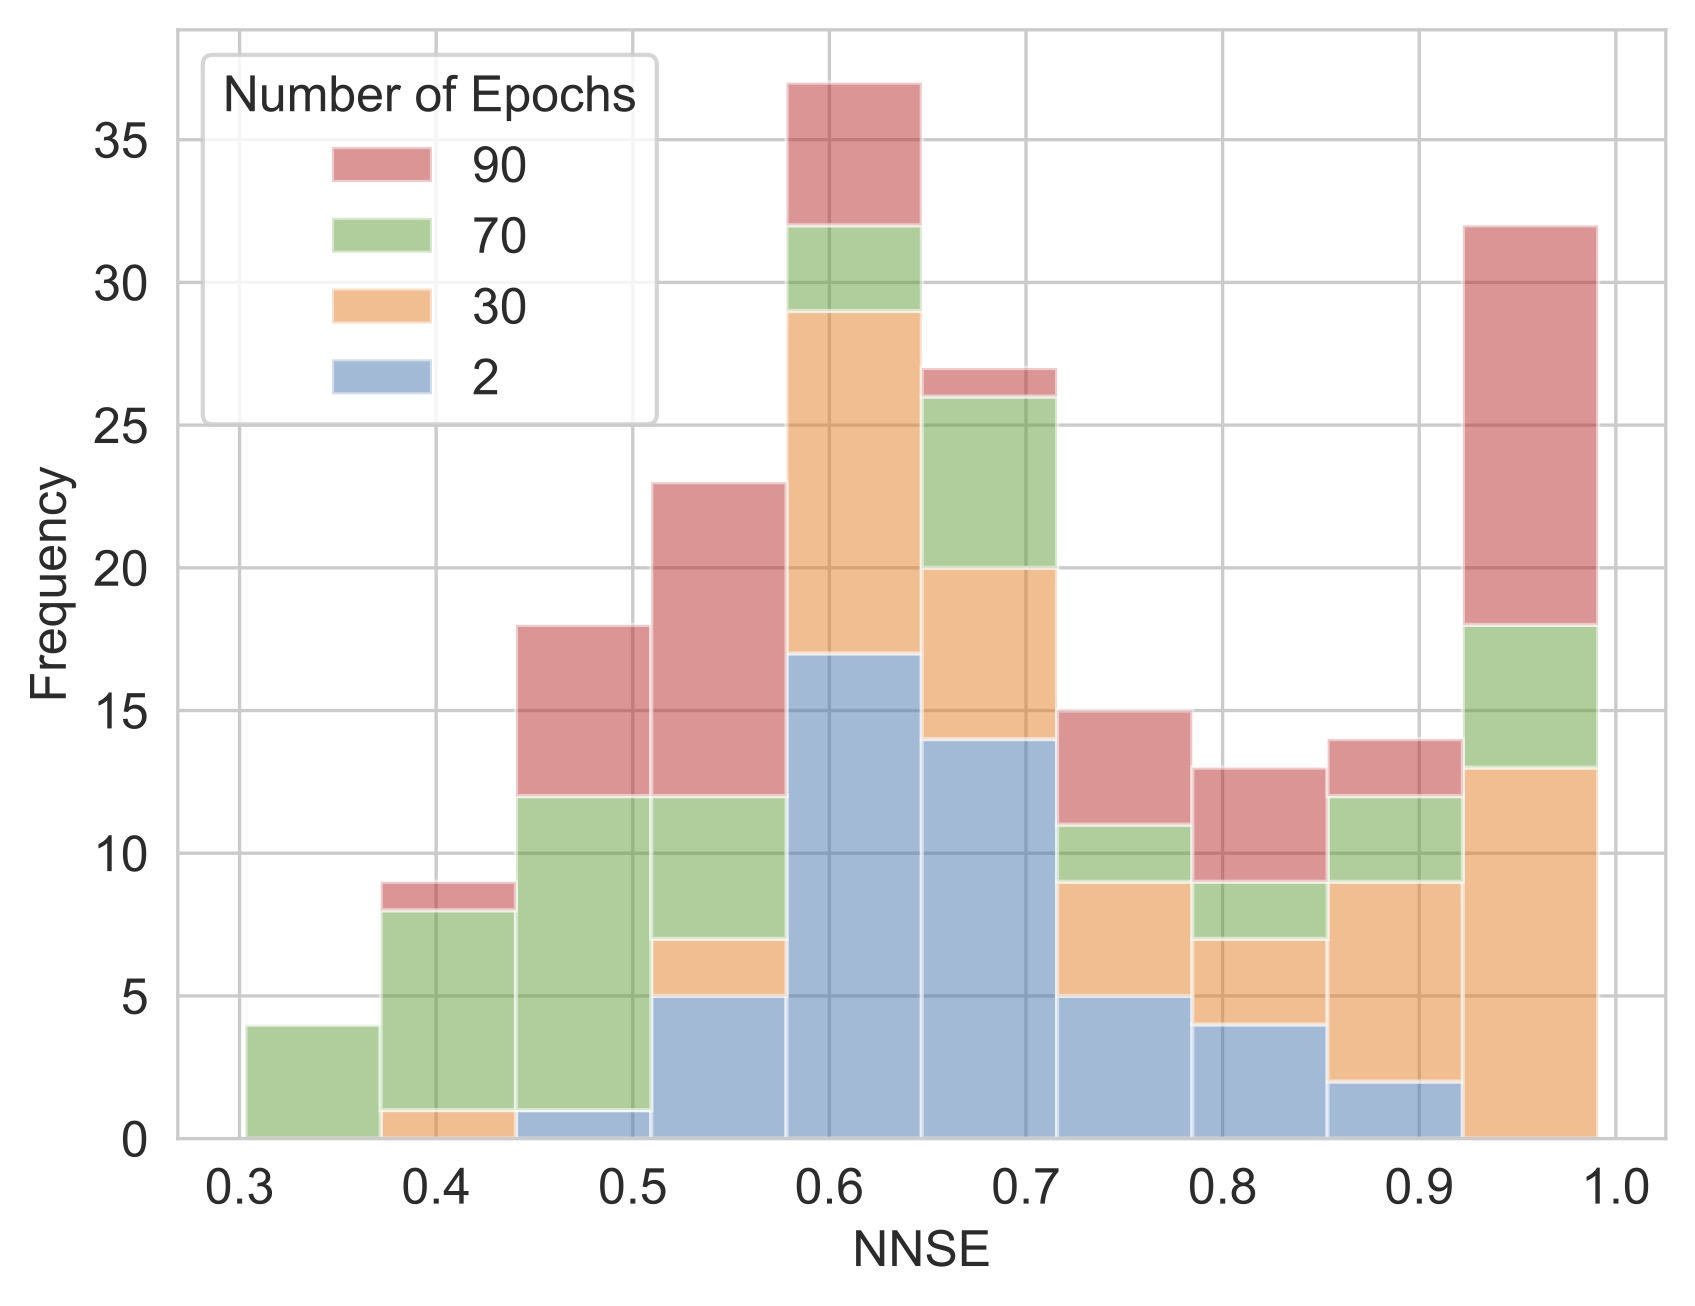
\includegraphics[width=1.0\linewidth]{images/frequency_nnse_histogram_stacked_df_validation_summed}
        {\bf (B)} Histogram of the summed accuracy values for every epoch over all experiments for validation.
     \end{minipage}
  \ \
     \begin{minipage}[t]{0.49\textwidth}
        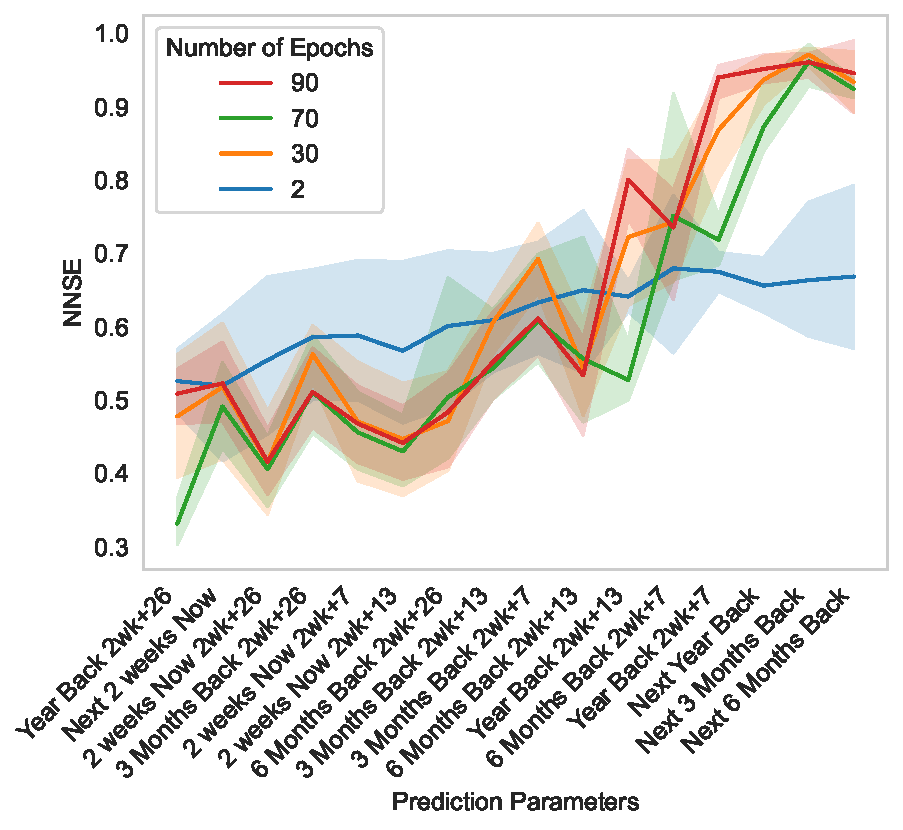
\includegraphics[width=1.0\linewidth]{images/NNSE-all-epochs-training-summed}
        {\bf (C)} Summed accuracy values over all experiments for training sorted by best training values.
     \end{minipage}
  \ \
     \begin{minipage}[t]{0.49\textwidth}
        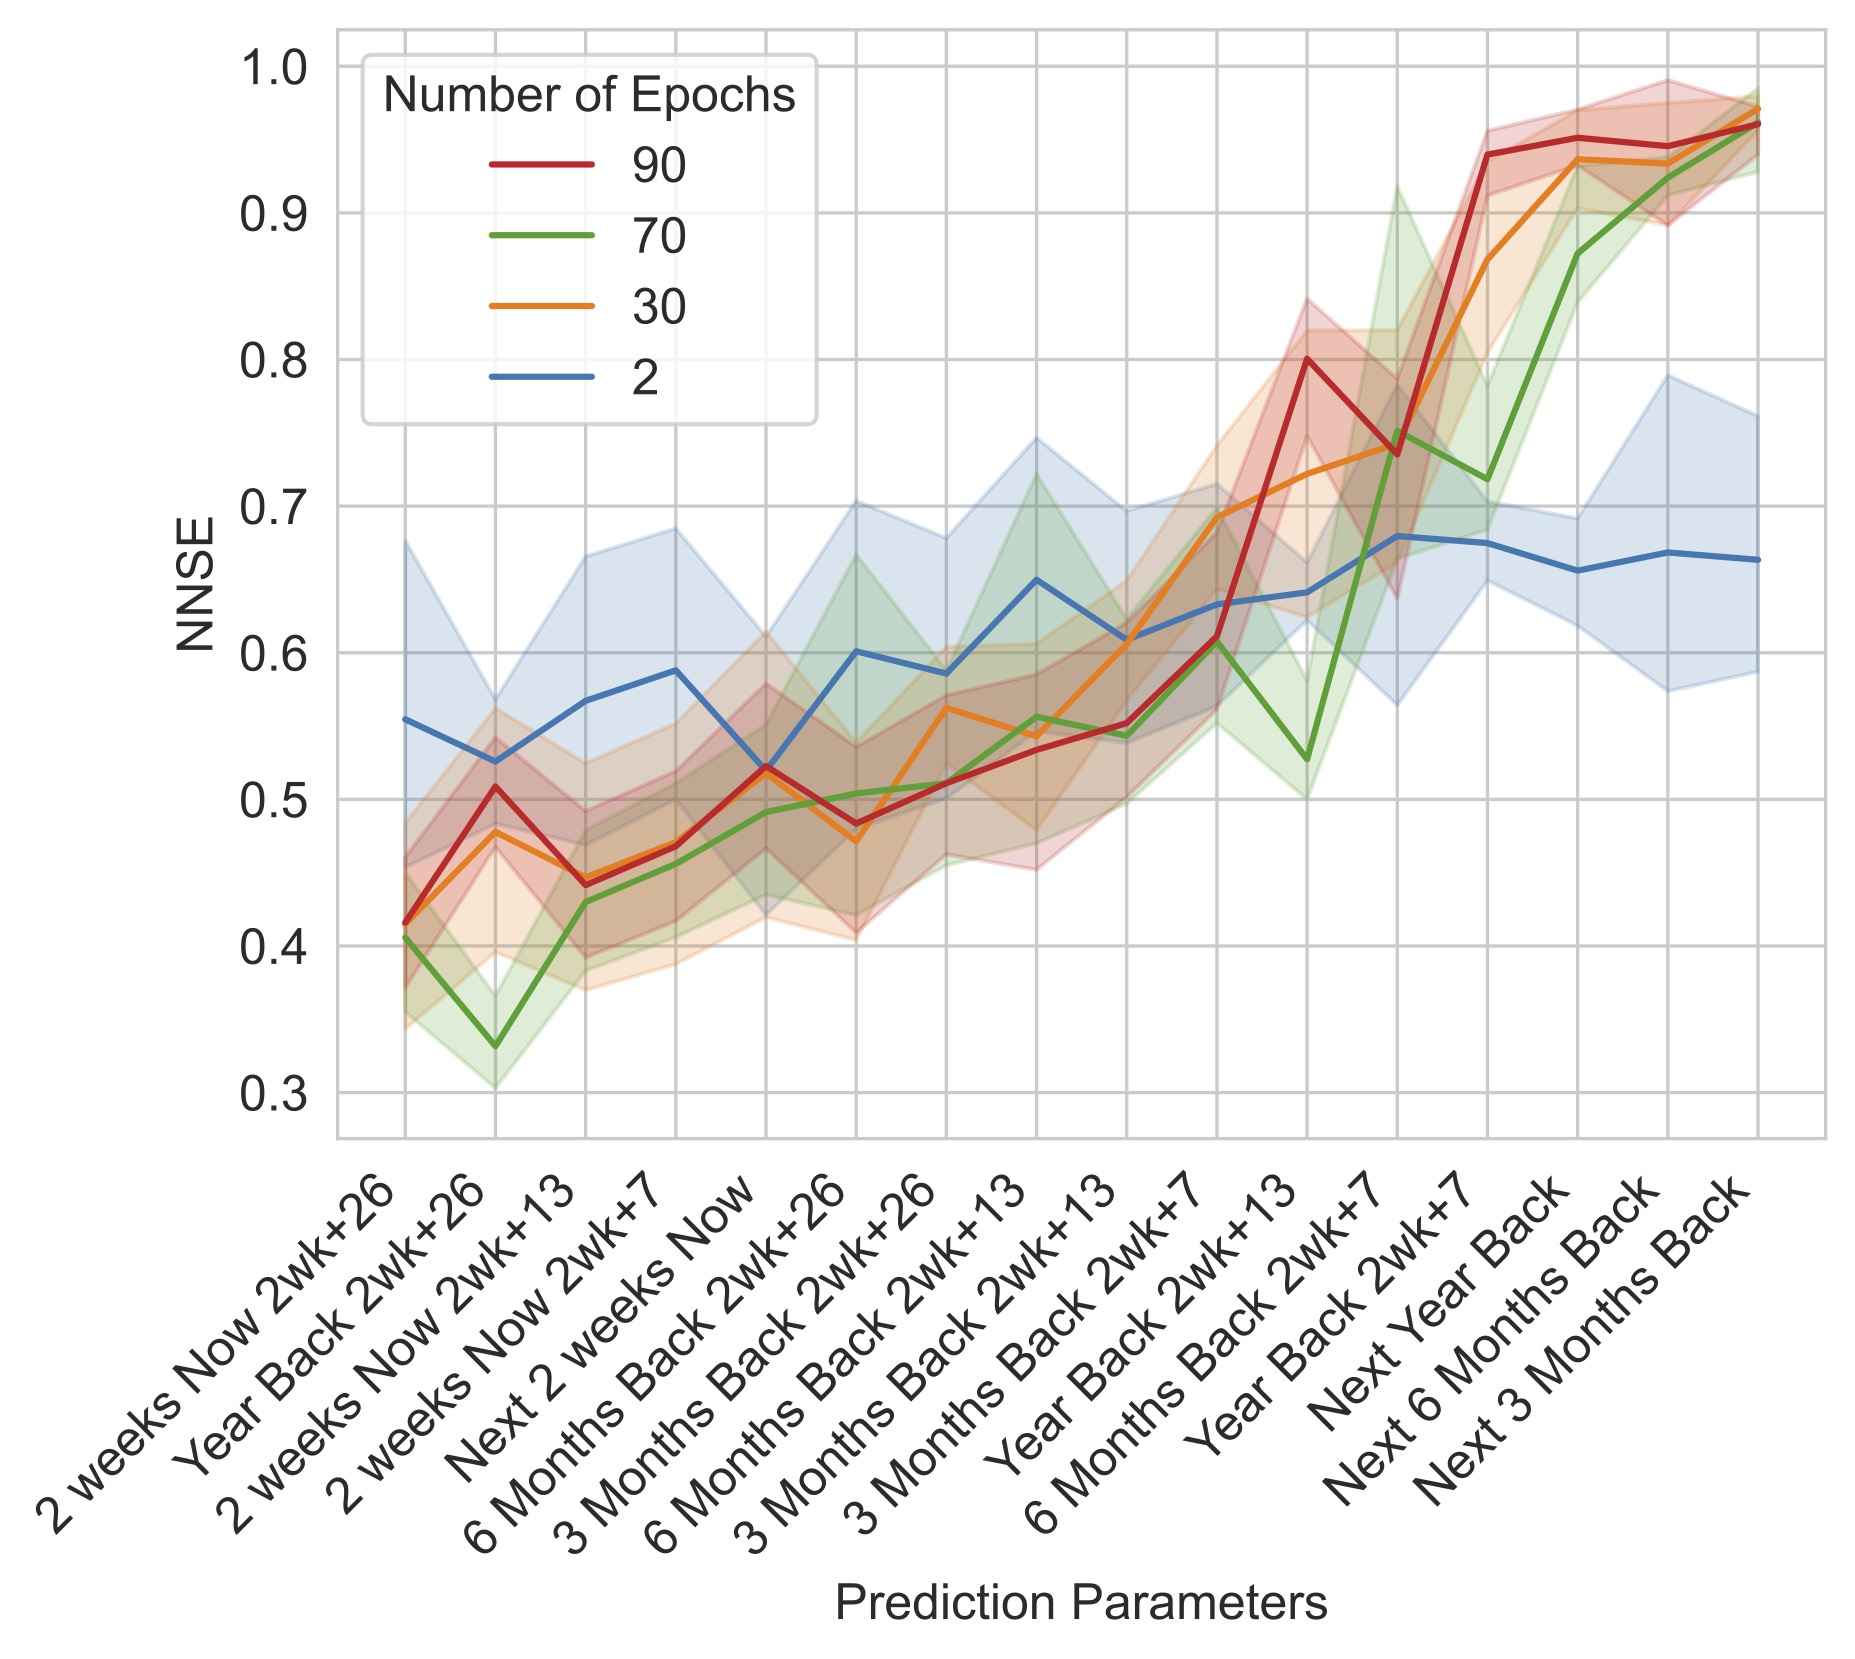
\includegraphics[width=1.0\linewidth]{images/NNSE-all-epochs-validation-summed}
        {\bf (D)} Summed accuracy values over all experiments for validation sorted by best validation values.
     \end{minipage}

  \end{center}

  \caption {Evaluation of the NNSE summed accuracy for epochs 2, 30, 70, and 90.}
  \label{fig:NNSE-comparison-a100-summed}

\end{figure}

\subsubsection{Energy}
\label{sec:perf-energy}


Energy consumption has become an important factor in the evaluation of computing centers due to the high costs associated with running them on large- scale. This not only includes common compute center-based metrics such as {\em Power Usage Effectiveness} (PUE) but also the measurement of application-oriented energy consumption.  Such application-oriented comparisons have led to a ranking of the most energy-efficient supercomputers as detailed in the Green500 list \citep{green500}. In such comparisons, the metric Energy Efficiency is used and derived by the GFlops/watts value. Just like TOP500, this benchmark is based on Linpack performance measurements \cite{www-top500}.  However, it is important to also consider other applications when measuring energy consumption. Such applications may consist of many different phases and may not perform at the maximum potential performance of the available hardware, or the available hardware may project a bottleneck for the performance.

To measure the algorithm's energy consumption we need to augment the application in such a way that we can monitor energy use over the lifetime of the application. For this, we have developed a simple-to-use energy trace program to monitor and predict our energy uses called \verb|cloudmesh-gpu| as introduced in Section \ref{sec:monitoring}.  We used for our initial experiments data hosted on an NFS filesystem in the data center as localscratch was not available at the time.


With this program, we can create energy traces of the GPU. An energy trace is a sample of energy measurements periodically taken over time of the GPU. The period of the measurements can be decreased to increase the accuracy of the energy measurements over time. Our presentation here only includes measurements of the GPU and does not include the measurement of the servers, file system, or network energy consumption as our focus for this study is the impact on GPUs and to see if they are efficiently used.

In our case, we chose to measure the GPU energy every second leading to an energy trace that we term $E^T_{\Delta t=1s}(GPU)$. Such traces can be applied to the application running with different hyperparameters. To showcase the drastically different energy traces we have limited our discussion to running applications on different GPUs (A100, V100) and different epochs (2, 30, 70). These traces are depicted in Figure~\ref{fig:energy-graphs}A-F.  To better showcase the impact of the different phases of the application we have augmented the traces with different colors for the different phases of the application.  We distinguish the phases called {\em Initialize}, {\em Training}, {\em Best Fit Prediction}, {\em Visualize}, and {\em Final plots}. The meaning of these phases has been explained in Section~\ref{sec:perf-runtime}. And used different colors for the phases in the Figure~\ref{fig:energy-graphs} to distinguish them better.

An important observation is for the training phase (colored in green) the energy values of the GPU are significantly higher than in the rest of the application indicating a much higher utilization of the GPU during that phase.

The other phases dealing with data reparation only show a modest use of the GPU. We have measured the energy consumption between different GPUS.  When looking at the energy traces Figure~\ref{fig:energy-graphs} showing the differences between A100 and the V100 GPUs we note that the time on the abscissa is significantly larger for the V100. Hence overall energy consumption per second will be significantly larger. The fluctuations of the energy in the training phase can be explained through the various repeated processes that exist within the training of DL application.

%\TODO{All}{Figure 9 A, B, C needs in the graphs to have labels A100, V100 P100, K80, e.g. capital letter}

To compare the energy values between different GPUs such as A100, V100, and P100 we can calculate the {\em Energy Trace Consumption} defined as the sum of all Energy values in an energy trace $E^T_C \sum E^T_{\Delta t=1s}(GPU)$ applied to a hyperparameter such as the epoch.  We can then calculate the energy trace consumption per epoch which we plotted in Figure~\ref{fig:energy-graphs-compare}A.  As the time with higher epoch numbers is dominated by the training time as seen in Figure~\ref{fig:energy-graphs}.  Hence the energy per epoch for lower numbers of epochs will be small, while for larger numbers the energy per epoch will be higher. However, they will not change much with higher numbers of epochs as demonstrated in Figure~\ref{fig:energy-graphs-compare}A.  We also see that the K80 uses significantly higher energy than the other GPUs, with the A100 performing best. For K80 and 70 epochs, we could not obtain a value as it was outside the allowed time to run applications on the supercomputer defined by the center's policy.  We also see that the standard deviation for the kWh/Epoch value becomes smaller with an increasing number of epochs.

This means that the power usage of GPUs is generally constant when training our benchmark model and could be used for energy prediction.



In Figure~\ref{fig:energy-graphs-compare}B, we also depicted the Energy trace per epoch. However, in contrast to Figure~\ref{fig:energy-graphs-compare}A that were created using the data on an NFS storage device, we included here the values obtained for data hosted on a localscratch filesystem and the project filesystem. While the localscratch uses NVMe storage the project filesystem is hosted on a shared GPFS storage server. Accessing the data from there takes more time and hence more energy is used during the benchmark per epoch.

Hence it offers a clear insight into how a filesystem can negatively impact the energy as the runtime is enhanced and the GPU time to cool down or adjust for reducing the energy is too small to have an impact.


Additionally in Figure~\ref{fig:energy-graphs-compare}C, we see the total GPU energy consumption from the complete execution of the benchmark notebook depicting measures from the phases {\em Initialize}, {\em Training}, {\em Bestfit Prediction}, {\em Visualize}, and {\em Final Plots}.  This graph is important, as it shows the impacts of the energy usage of the GPU throughout the runtime and when compared to the plots in Figure~\ref{fig:energy-graphs-compare}A and \ref{fig:energy-graphs-compare}B, outlier events, such as a potential interaction from other users sharing the benchmark infrastructure can be identified.


\begin{figure}[htb]

  \begin{center}

     \begin{minipage}[b]{0.43\textwidth}
       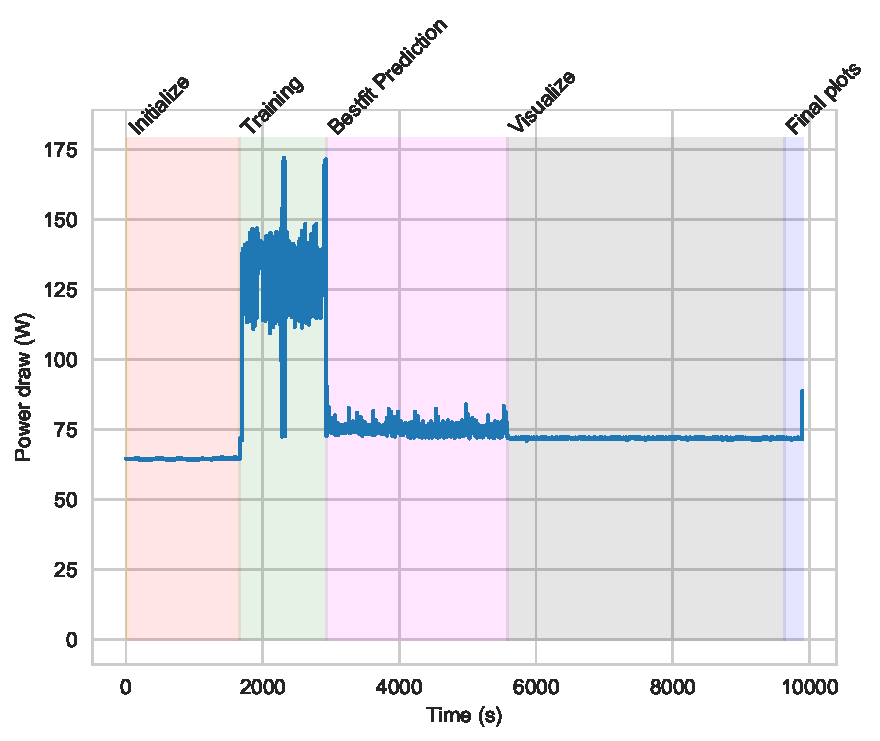
\includegraphics[width=1.0\linewidth]{images/a100-shaded-energy-2-epochs}
        {\bf (A)} A100 energy trace $E^T_{\Delta t=1s}(GPU)$ for 2 epochs training and validation.
    \end{minipage}
     \ \
     \begin{minipage}[b]{0.43\textwidth}
        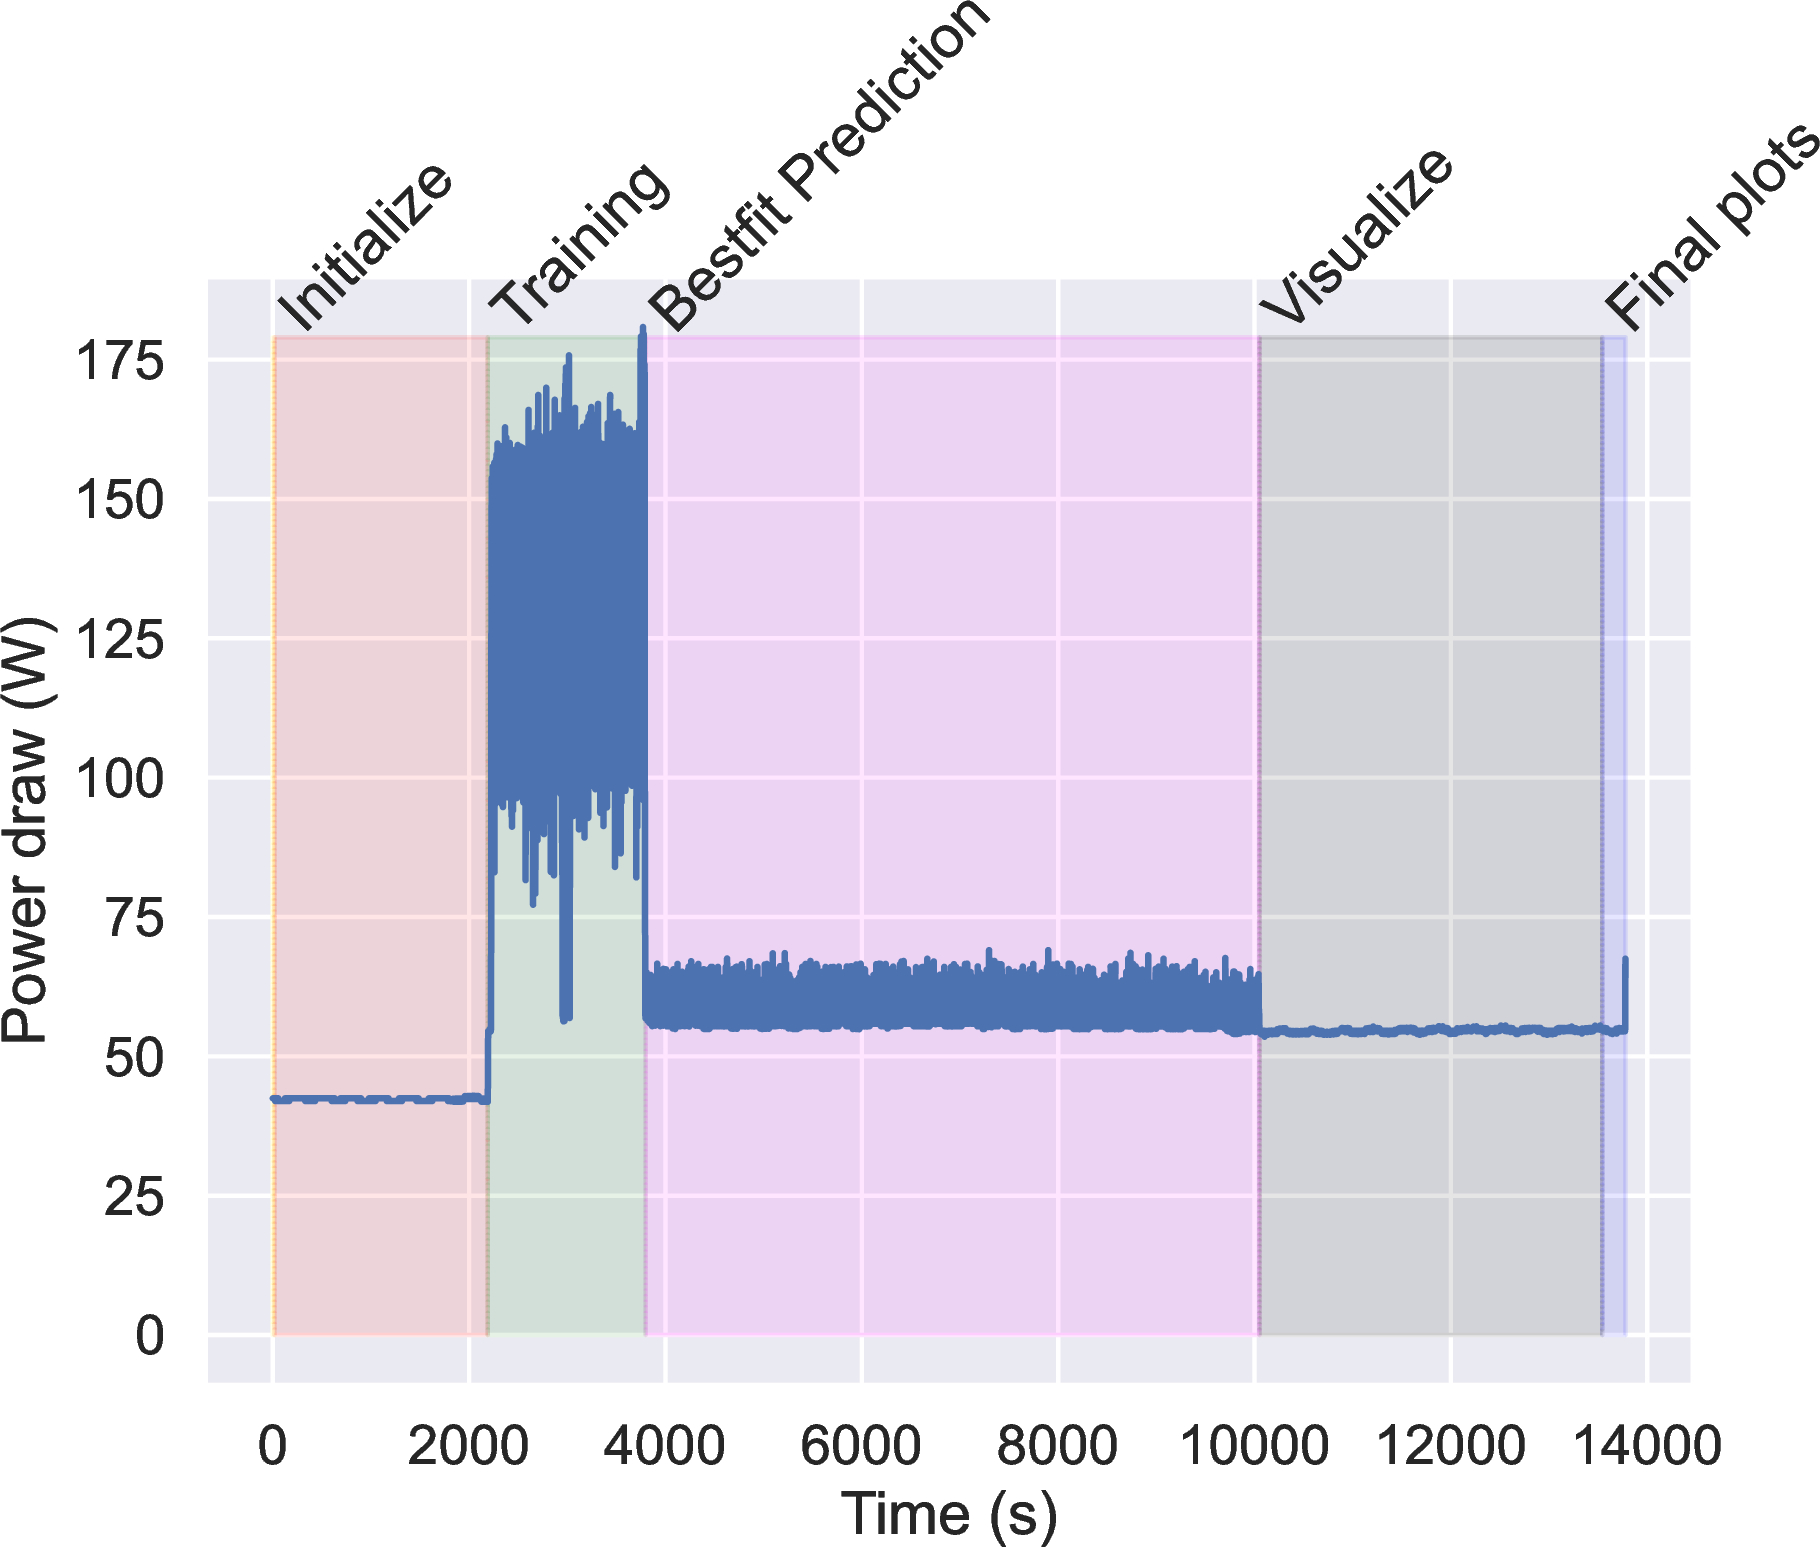
\includegraphics[width=1.0\linewidth]{images/v100-shaded-energy-2-epochs}
        {\bf (B)}  V100 energy trace $E^T_{\Delta t=1s}(GPU)$ for 2 epochs training and validation.
     \end{minipage}

     \begin{minipage}[b]{0.43\textwidth}
        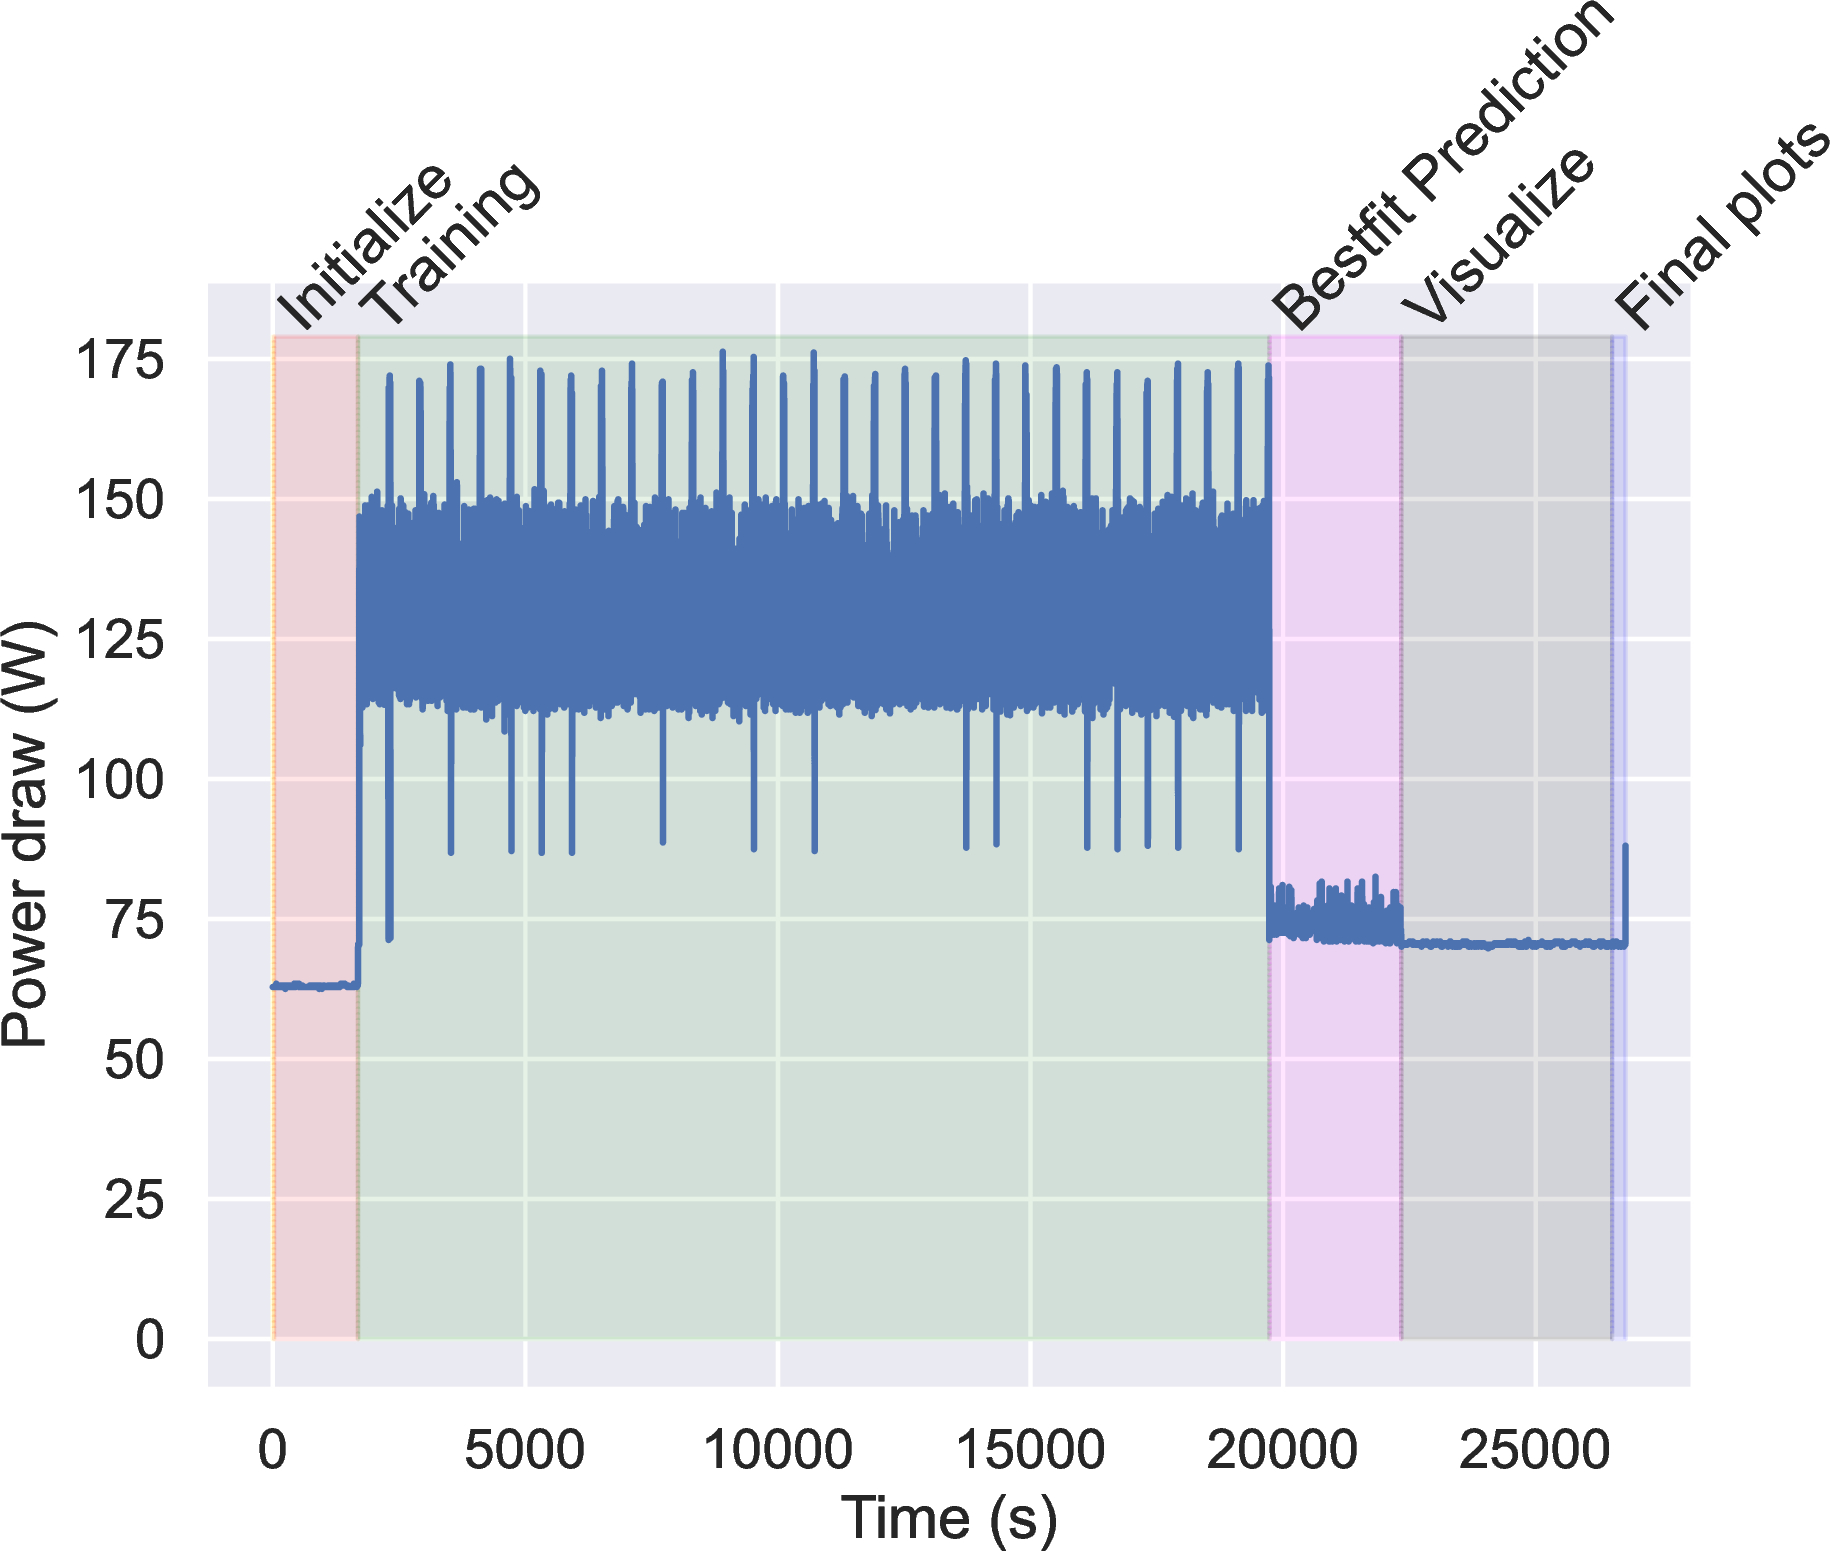
\includegraphics[width=1.0\linewidth]{images/a100-shaded-energy-30-epochs}
        {\bf (C)} A100 energy trace $E^T_{\Delta t=1s}(GPU)$ for 30 epochs training and validation.
     \end{minipage}
     \ \
     \begin{minipage}[b]{0.43\textwidth}
        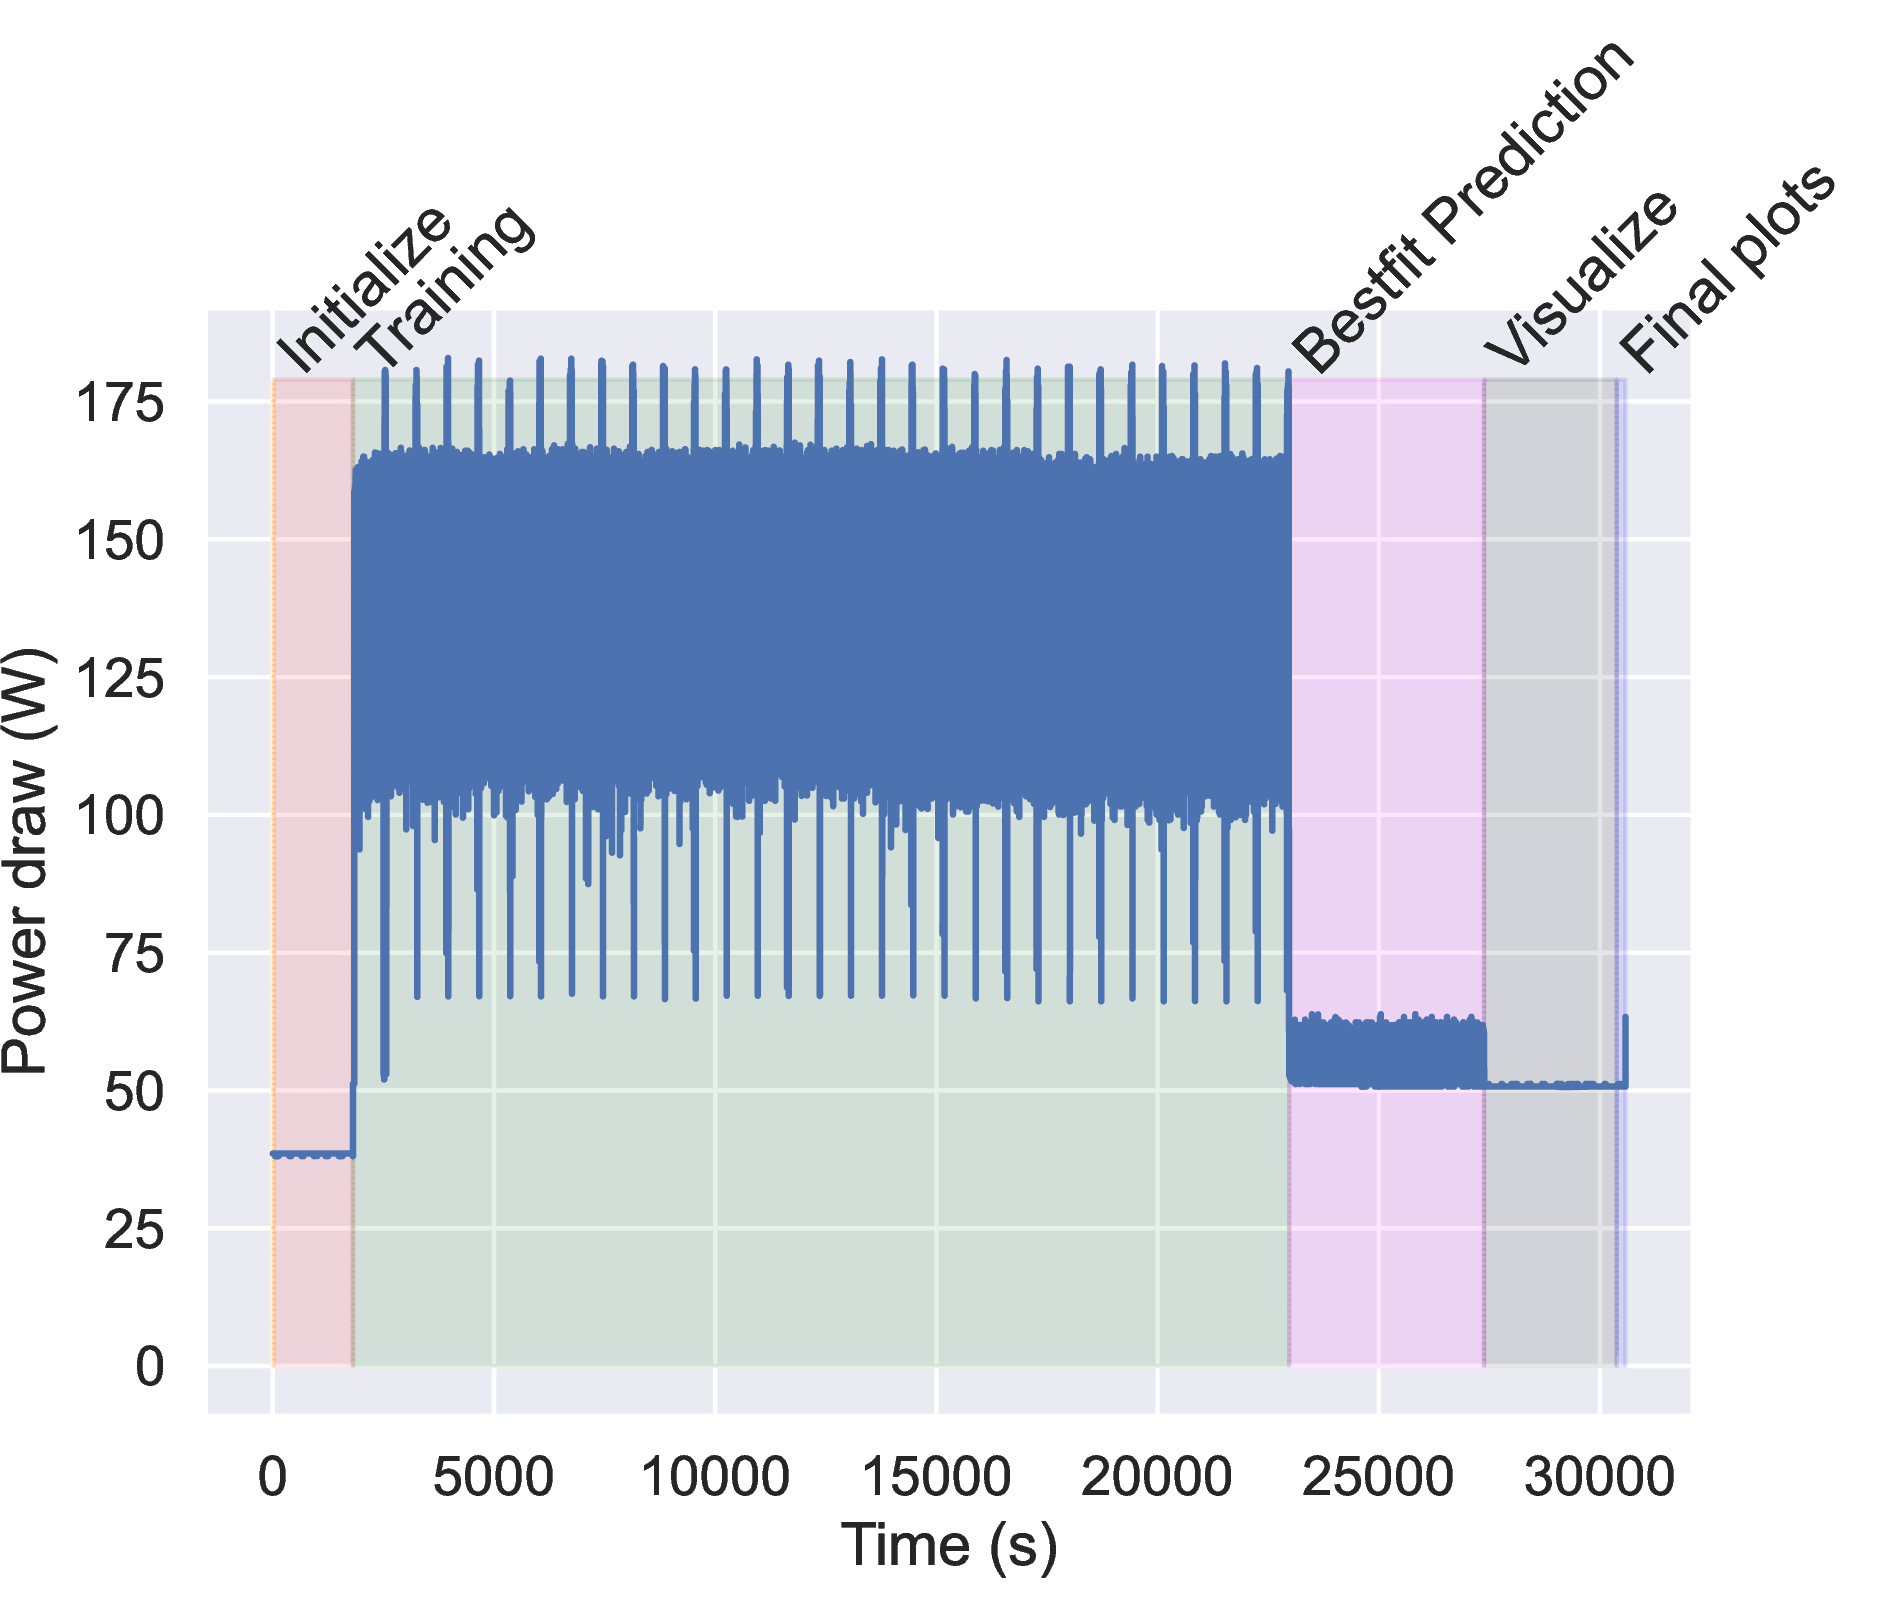
\includegraphics[width=1.0\linewidth]{images/v100-shaded-energy-30-epochs}
        {\bf (D)} V100 energy trace $E^T_{\Delta t=1s}(GPU)$ for 30 epochs training and validation.
     \end{minipage}

     \begin{minipage}[b]{0.43\textwidth}
       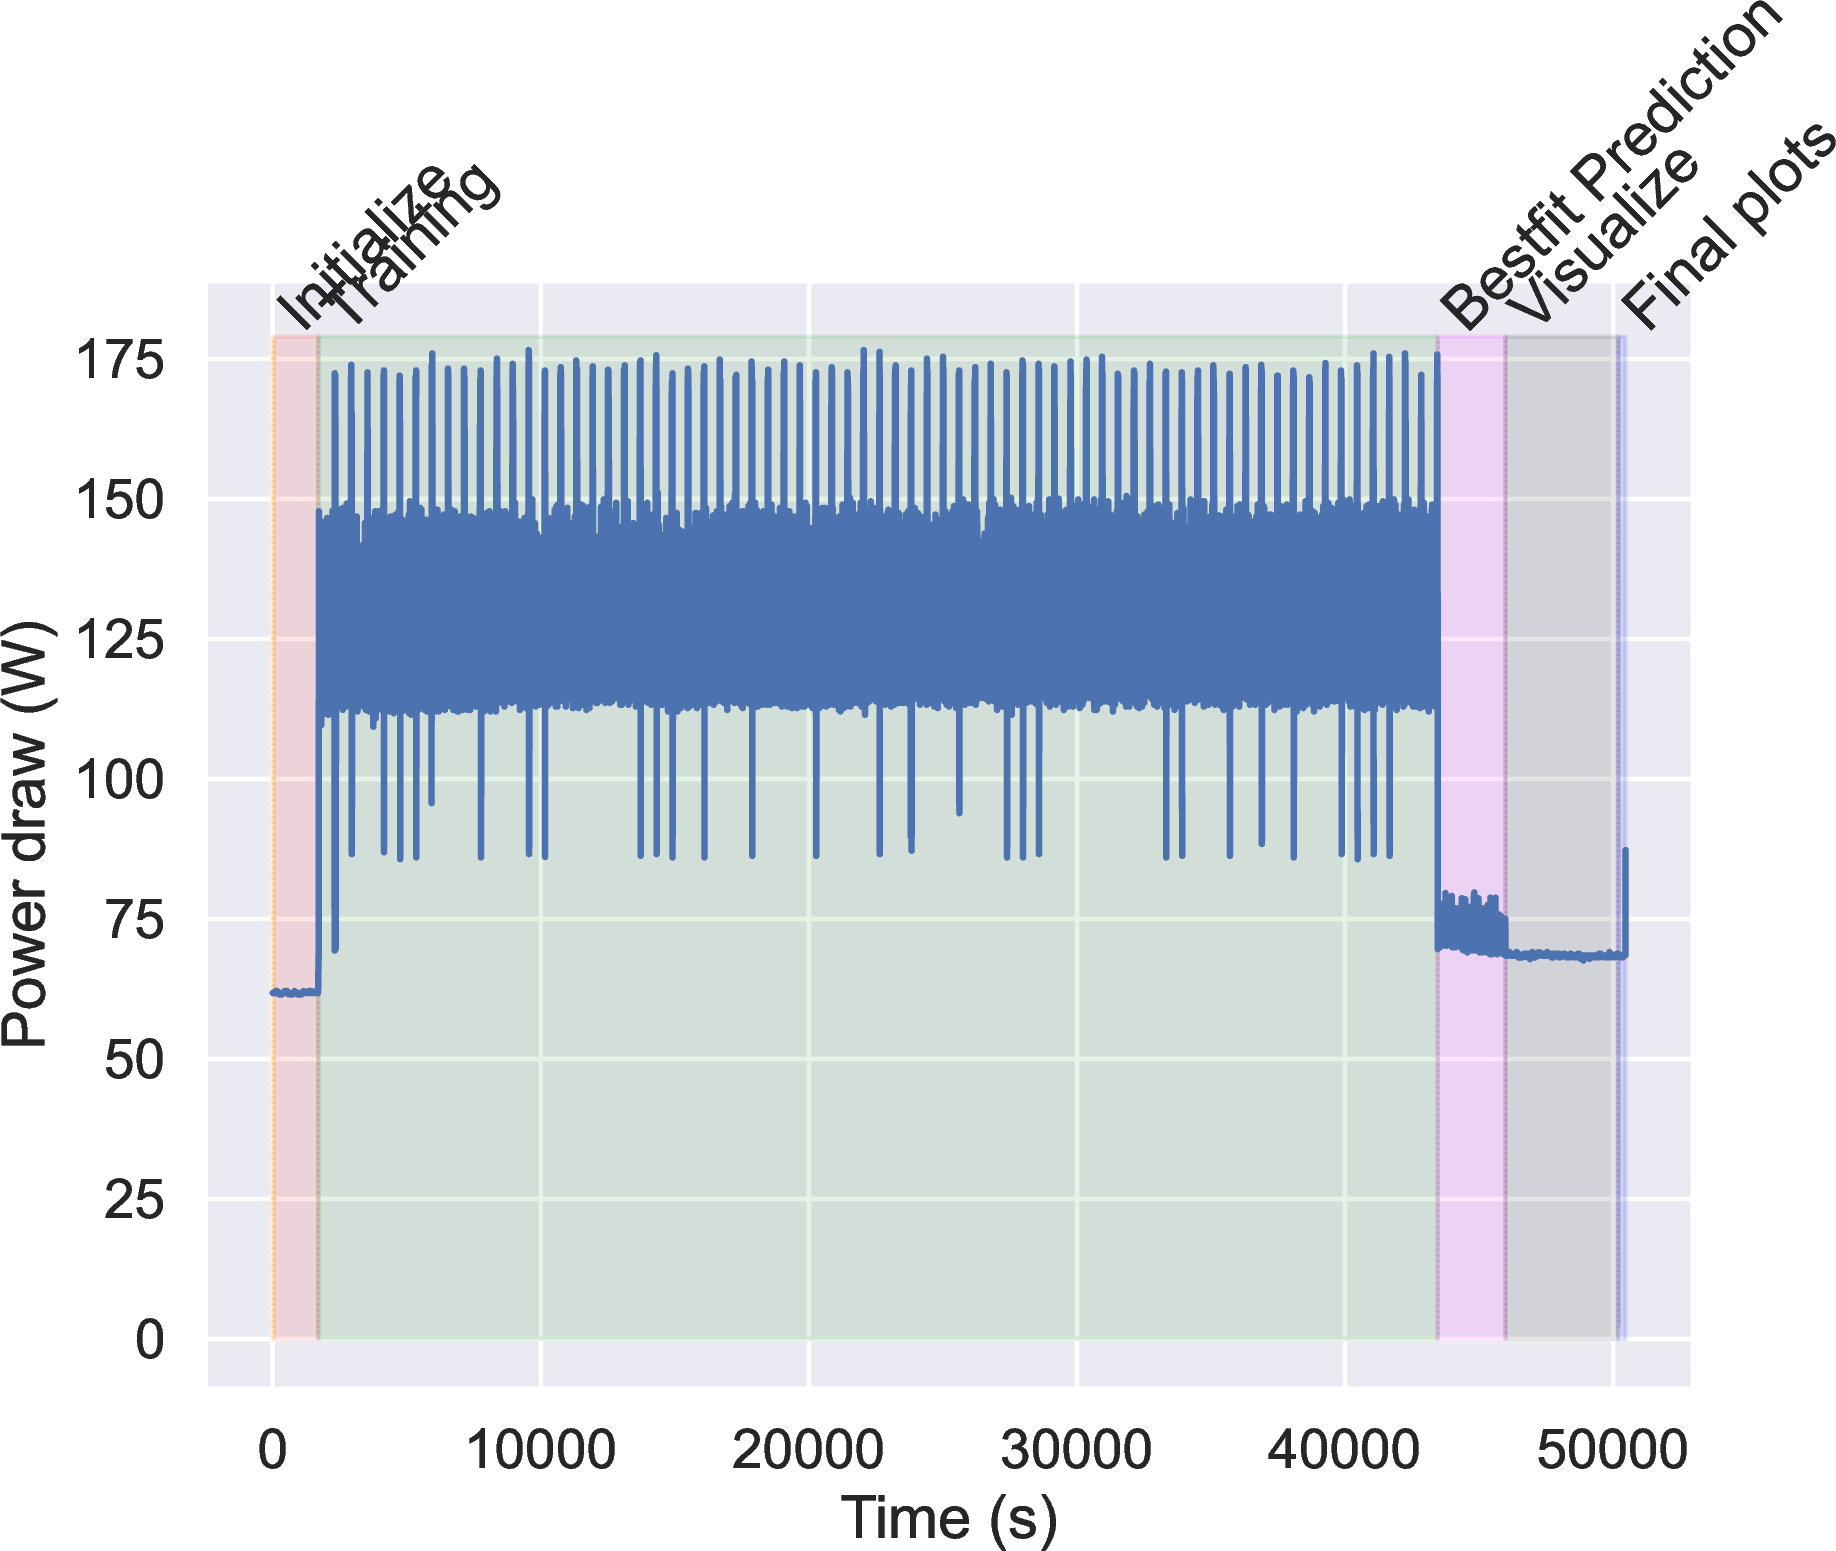
\includegraphics[width=1.0\linewidth]{images/a100-shaded-energy-70-epochs}
        {\bf (E)} A100 energy trace $E^T_{\Delta t=1s}(GPU)$ for 70 epochs training and validation.
     \end{minipage}
     \ \
     \begin{minipage}[b]{0.43\textwidth}
        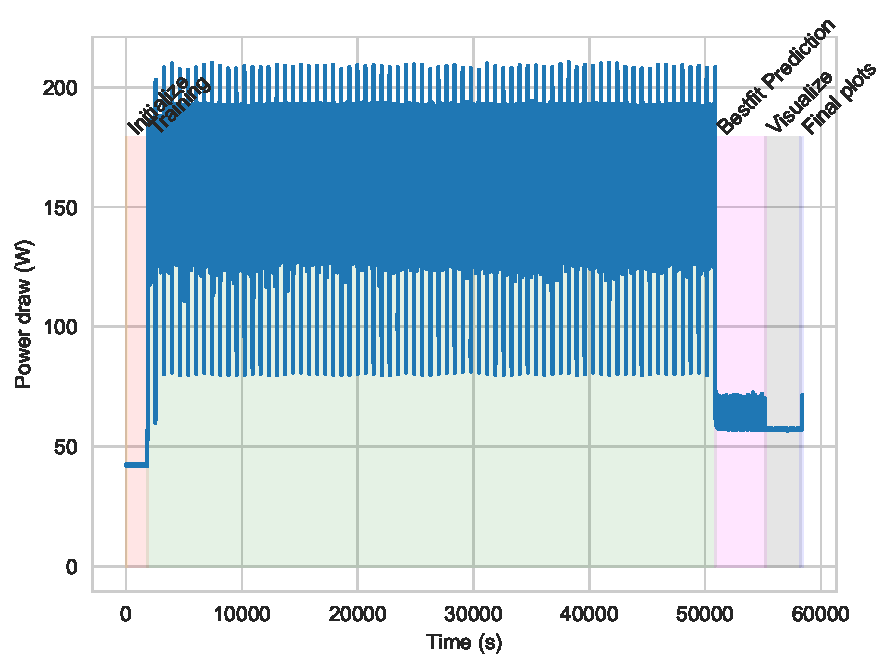
\includegraphics[width=1.0\linewidth]{images/v100-shaded-energy-70-epochs}
        {\bf (F)}  V100 energy trace $E^T_{\Delta t=1s}(GPU)$ for 70 epochs training and validation.
     \end{minipage}
\end{center}

     \caption{Energy traces for training and validation for epochs 2 (A, B), 30 (C, D), 70 (E, F). The sampling rate is 1 second.}
     \label{fig:energy-graphs}
\end{figure}



\begin{figure}[htb]

  \begin{center}

       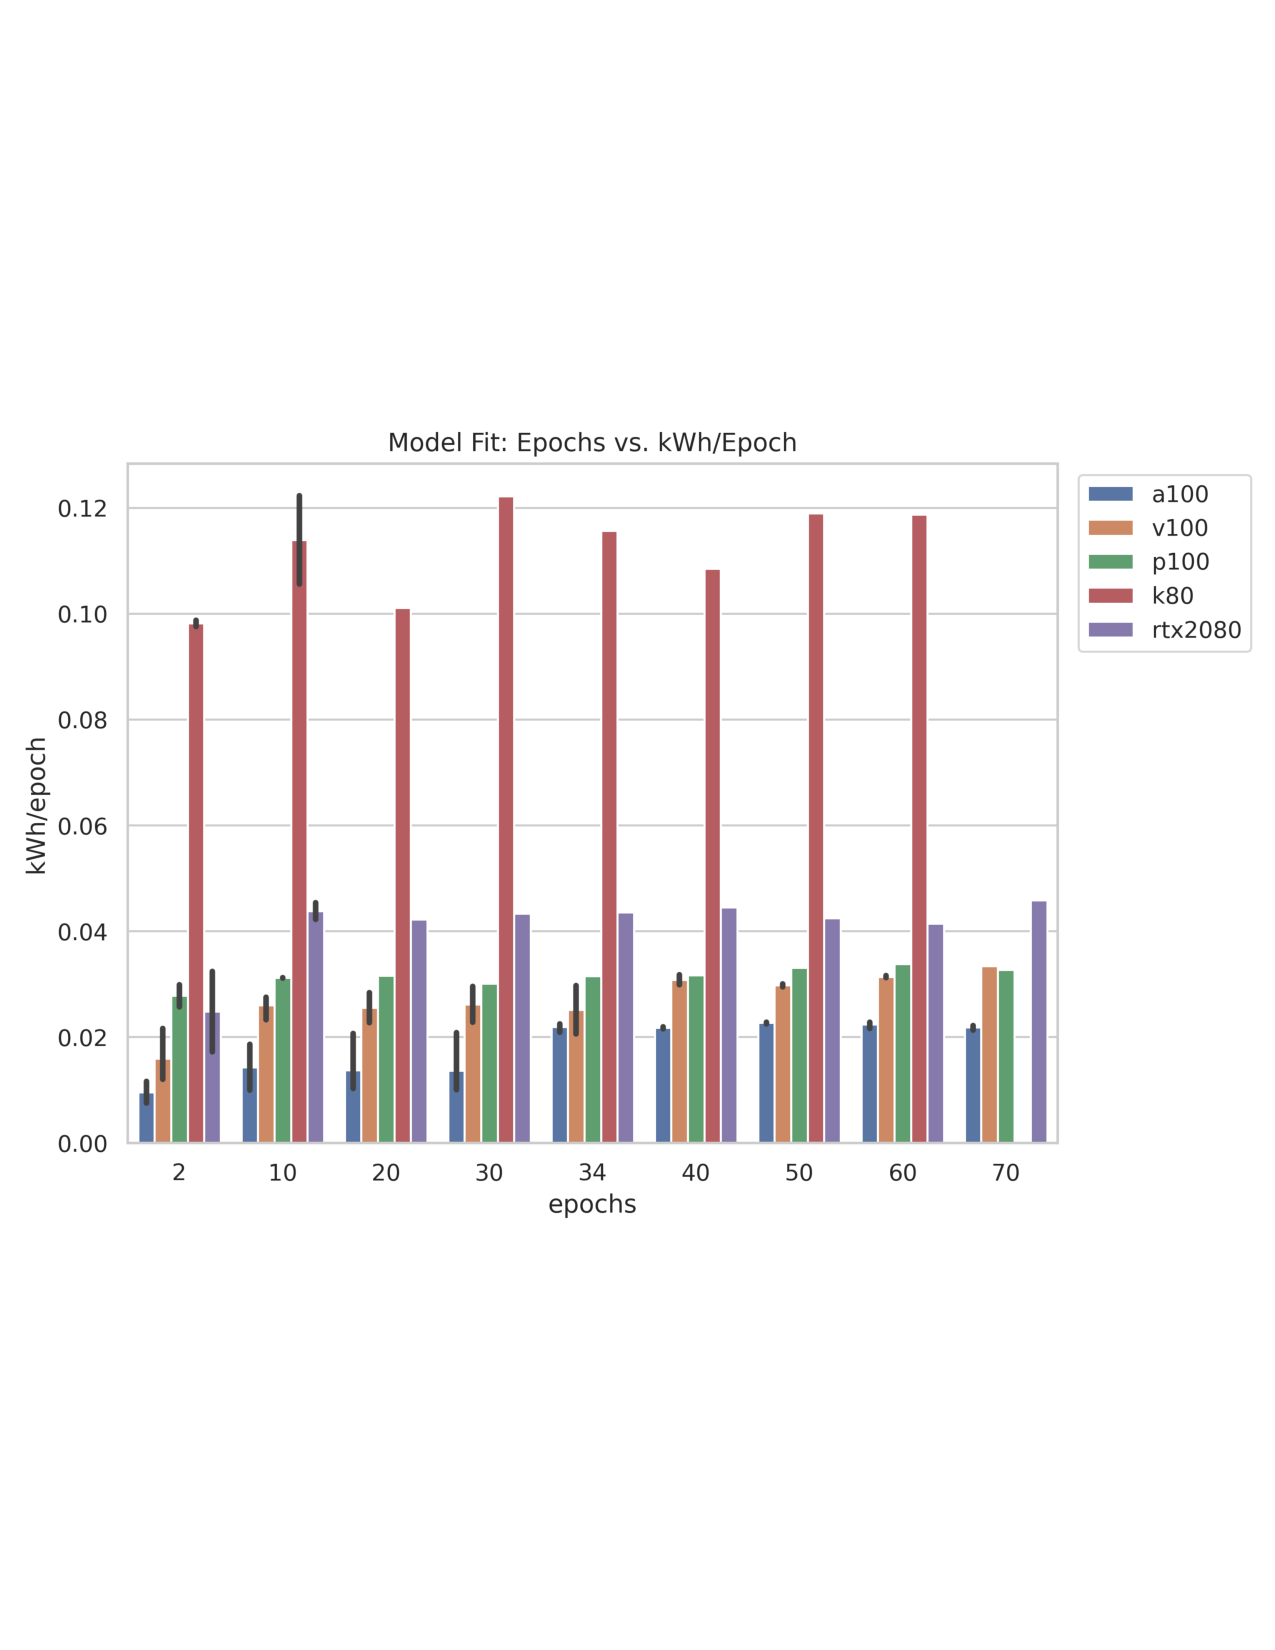
\includegraphics[height=0.28\textheight]{images/energy_all_model_fit_kWh_per_epoch}

       {\bf (A)} Average energy usage per epoch, including only to the Training event energy traces

        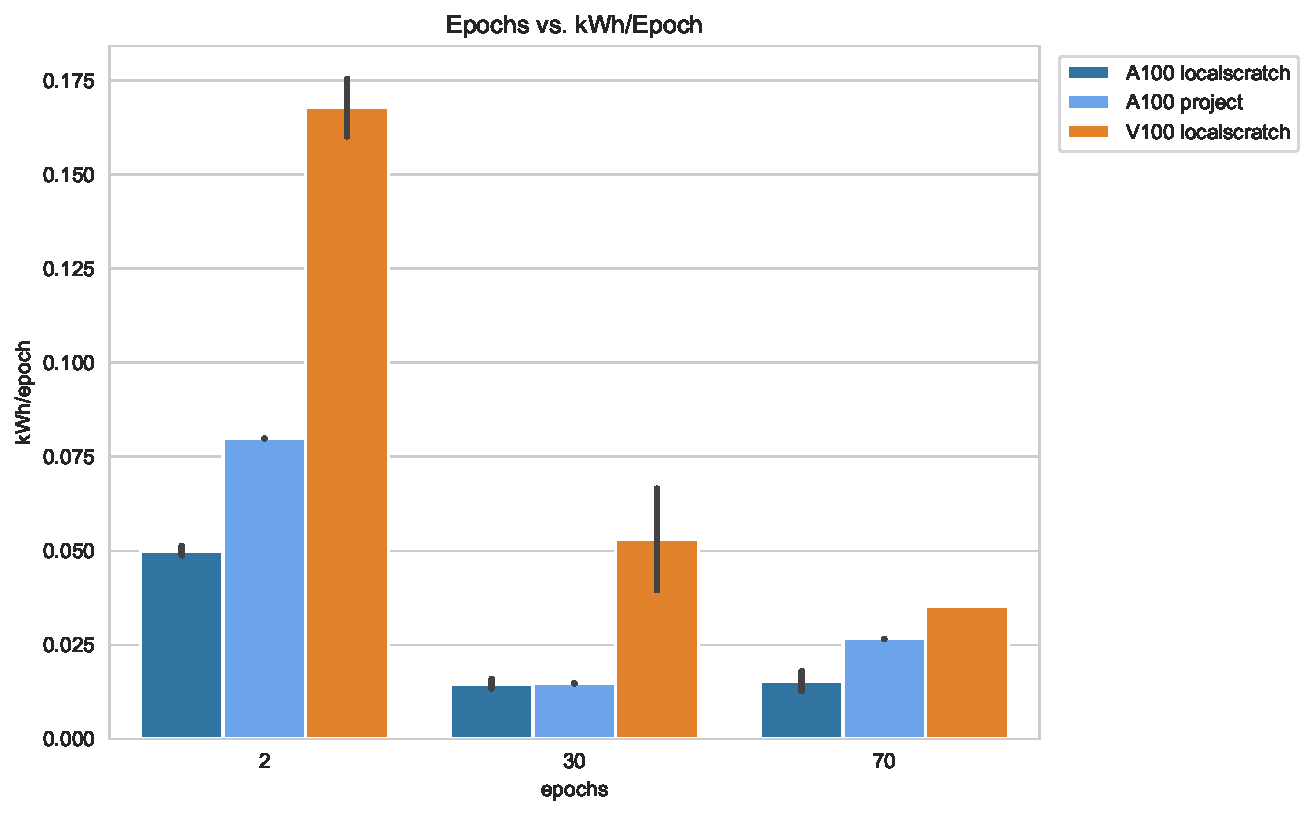
\includegraphics[height=0.29\textheight]{images/total_kWh_per_epoch_new}

         {\bf (B)} Average energy usage per epoch, for all energy traces for all timer events.

        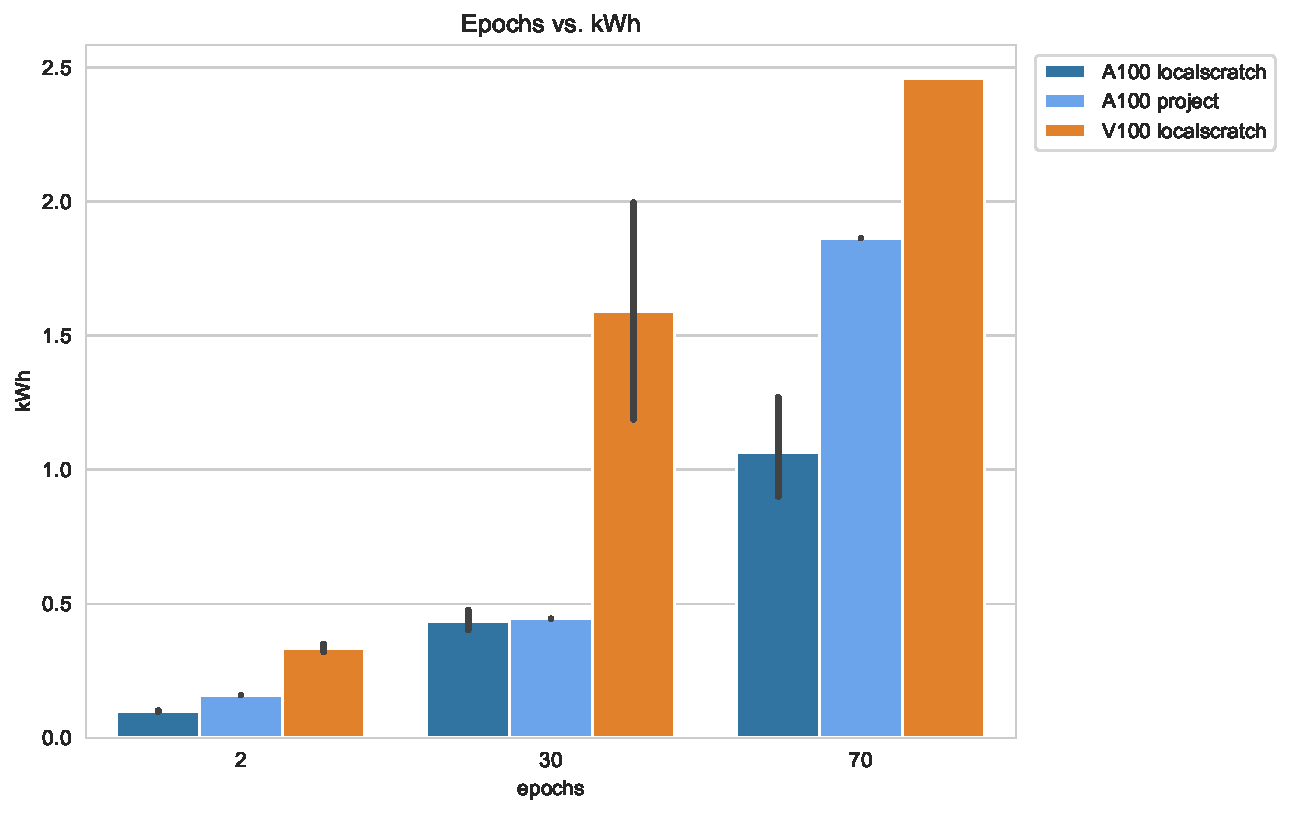
\includegraphics[height=0.28\textheight]{images/total_epoch_vs_watts_new}

        {\bf (C)} Average energy usage for all energy traces for all timer events.


  \end{center}

  \caption{Averaged energy consumption of various GPUs targeting a 1 second data sampling rate. The recorded values in (A) and all V100 reported are produced with an NFS mounted filesystem.  The data for A100 in (B) and (C) is using localscratch's NVMe storage.} 
  \label{fig:energy-graphs-compare}
\end{figure}



\section{Discussion}
\label{sec:conclusion}

% \TODO{GVL}{enhance the discussion section}

This paper summarizes a large body of work that addresses multiple aspects of machine learning benchmarking. We identified that benchmarking can lead to a significant educational contribution to students and researchers. We identified that not only is software carpentry needed, but also {\em benchmark carpentry}, an effort that we termed in conjunction with the MLCommons Science Working Group. We have demonstrated that students are capable of conducting sophisticated benchmarks while dealing with complex system-related infrastructure and working with policies set by HPC compute centers that deal with fair resource management. To deal with this we have also developed a compute coordination and workflow management system in two components called \verb|cloudmesh-sbatch| and \verb|cloudmesh-cc| that allow benchmark jobs to be automatically generated from hyperparameter permutations. It also allows us to coordinate such benchmarks on different machines. We have identified the patterns of selection, cooperation, and competition which are part of a benchmark workflow. Furthermore, we have improved the original benchmark code in many aspects. To simplify benchmarking we also developed an easy-to-use \verb|StopWatch| that in contrast to the \verb|mllog| library used by MLCommons is simpler and is immediately humanly readable. Lastly, our benchmarks had a significant impact on the operation and accessibility of software in the educational cluster we used. Plans for new filesystem management and updated compute nodes excite us to conduct more such studies. We intend to submit our results to the MLCommons Science Working groups as earthquake forecasting is one of their benchmark codes and efforts.


%%%%%%%%%%%%%%%%%%%%%%%%%%%%%

\begin{comment}
\TODO{TODO}

{\footnotesize
\begin{verbatim}
Cloudmesh Data Submodule - https://github.com/cloudmesh/cloudmesh-data
Cloudmesh GPU Submodule - https://github.com/cloudmesh/cloudmesh-gpu
Cloudmesh sbatch Submodule - https://github.com/cloudmesh/cloudmesh-sbatch 
\end{verbatim}
}
\end{comment}


%%%%%%%%%%%%%%%%%%%%%%%%%%%%%%%%%%%%%%%%%%%%%%%%%%%%%%%%%%%%%%%%%%%%%%%%%%%%%%%
\clearpage

\section{Nomenclature}

\subsection{Resource Identification Initiative}

{\bf Organization:} \verb|RRID:SCR_011743|

\section*{Conflict of Interest Statement}

The authors declare that the research was conducted in the absence of any commercial or financial relationships that could be construed as a potential conflict of interest.

\section*{Author Contributions}

{\em GvL} is the lead author and main contributor to this paper. He has modified and augmented the earthquake paper to include the ability to execute hyperparameters. {\em JPF} is a student that has contributed to various aspects of the workflow component of the paper and to a number of executions and evaluations of experiment runs. {\em RK} was a data-science student and has helped together with {\em GVL} in the implementation of cloudmesh-sbatch and the porting of the effort to the UVA machine.  {\em GCF} is the author of the earthquake code and facilitates the interactions with the MLCommons Science Working group as a group leader of that effort. {\em TB} and {\em JK} participated in an earlier phase of the project that ported and improved an earlier version of the code while adding timers and the energy monitor developed by {\em GvL}. {\em JF} was enabling the students {\em RK}, {\em TB}, and {\em JK} to participate in this project and provided administrative supervision to meet the class expectations and requirements needed for their participation.

\section*{Funding}

Work was in part funded by the NSF CyberTraining: CIC: CyberTraining for Students and Technologies from Generation Z with the award numbers 1829704 and 2200409 and NIST 60NANB21D151T.  The work was also funded by the Department of Energy under the grant Award No. DE-SC0023452. The work was conducted at the Biocomplexity Institute and Initiative at the University of Virginia.

\section*{Acknowledgments}

We like to thank Thomas Butler and Jake Kolessar for their contributions during the capstone project while focusing on executing initial runs of the code, and experimenting with modifications to the code including logging. Please note that since this team finished their work, significant improvements have been made by the first authors of this paper.


\section*{Data Availability Statement}

The code is all in the public domain and available on GitHub at the following locations

\begin{itemize}

\item {\bf cloudmesh-cc} -- Is a code to control workflows to be executed on
  remote computing
  resources. \url{https://github.com/cloudmesh/cloudmesh-cc}

\item {\bf cloudmesh-sbatch} -- Is a code to generate batch scripts for
  hyperparameter studies high-performance computers so they can be
  executed on different supercomputers by multiple
  accounts. \url{https://github.com/cloudmesh/cloudmesh-sbatch}

\item {\bf cloudmesh} -- Cloudmesh is a large collection of repositories for
  accessing cloud and HPC
  resources. \url{https://github.com/orgs/cloudmesh/repositories}

\item {\bf MLCommons earthquake production code} -- The MLCommons Science
  Working group is described at
  \url{https://mlcommons.org/en/groups/research-science/}. This page
  contains the links to the production-level earthquake code.

\item {\bf MLCommons earthquake development code} -- The development version of
  the code is available in this repository. It also contains many of
  the analysis scripts that are not part of the production code
  hosted by MLCommons \url{https://github.com/laszewsk/mlcommons}.

\end{itemize}


% \bibliographystyle{Frontiers-Harvard}

\bibliographystyle{Frontiers-Vancouver} % Many Frontiers journals
% use the numbered referencing system, to find the style and resources
% for the journal you are submitting to:
% https://zendesk.frontiersin.org/hc/en-us/articles/360017860337-Frontiers-Reference-Styles-by-Journal

\bibliography{vonLaszewski-frontiers-citations}





\end{document}
